
\documentclass{article} % For LaTeX2e
\usepackage{iclr2027_conference,times}

% Optional math commands from https://github.com/goodfeli/dlbook_notation.
\input{math_commands.tex}
\usepackage{multirow}
\usepackage{url}
\usepackage{graphicx}
\usepackage{booktabs}
\usepackage{algorithm}      % 提供 algorithm 浮动环境
\usepackage{algorithmic}    % 提供 algorithmic 环境（含 \REQUIRE、\STATE、\FOR 等命令）
\usepackage{hyperref}

\title{When and Why Compression Makes LoRA Better: A Bias--Variance Theory of Compressed Adaptation}

% Authors must not appear in the submitted version. They should be hidden
% as long as the \iclrfinalcopy macro remains commented out below.
% Non-anonymous submissions will be rejected without review.

\author{Antiquus S.~Hippocampus, Natalia Cerebro \& Amelie P. Amygdale \thanks{ Use footnote for providing further information
about author (webpage, alternative address)---\emph{not} for acknowledging
funding agencies.  Funding acknowledgements go at the end of the paper.} \\
Department of Computer Science\\
Cranberry-Lemon University\\
Pittsburgh, PA 15213, USA \\
\texttt{\{hippo,brain,jen\}@cs.cranberry-lemon.edu} \\
\And
Ji Q. Ren \& Yevgeny LeNet \\
Department of Computational Neuroscience \\
University of the Witwatersrand \\
Joburg, South Africa \\
\texttt{\{robot,net\}@wits.ac.za} \\
\AND
Coauthor \\
Affiliation \\
Address \\
\texttt{email}
}

% The \author macro works with any number of authors. There are two commands
% used to separate the names and addresses of multiple authors: \And and \AND.
%
% Using \And between authors leaves it to \LaTeX{} to determine where to break
% the lines. Using \AND forces a linebreak at that point. So, if \LaTeX{}
% puts 3 of 4 authors names on the first line, and the last on the second
% line, try using \AND instead of \And before the third author name.

\newcommand{\fix}{\marginpar{FIX}}
\newcommand{\new}{\marginpar{NEW}}

\newtheorem{proposition}{Proposition}
\newtheorem{corollary}{Corollary}

%\iclrfinalcopy % Uncomment for camera-ready version, but NOT for submission.
\begin{document}


\maketitle

\begin{abstract}
Compressed LoRA can outperform standard LoRA with far fewer trainable parameters. Low-dimensional adaptation can preserve useful capacity, but capacity alone does not determine when restricting estimation improves generalization. We develop a bias--variance account of compressed LoRA that connects this statistical question to compression geometry. Under a local quadratic approximation, restriction exchanges estimation variance for task-dependent projection bias. An isotropic sequence model yields an exact condition: compression helps a fixed task when its residual energy per excluded dimension is below the effective estimation noise; an additional isotropic target average gives an ensemble condition. The analysis predicts success and failure regimes as sample size, noise, and residual geometry vary. Projection-blind sequence experiments verify the exact crossover, and a nonlinear Transformer teacher--student study tests its qualitative persistence. Real-model diagnostics reveal variance reduction and task-dependent bias recovery, while delimiting the sample-size prediction. As a constructive consequence, an equal-budget analysis motivates Projected LoRA with Sparse Adapter (ProLoSA), which restores informative residual directions. Language understanding, mathematical reasoning, and instruction-tuning experiments assess its practical benefits and limits. Together, these results provide a statistical explanation of compressed adaptation and a design principle for correcting its recoverable bias.
\end{abstract}

\section{Introduction}
Low-Rank Adaptation (LoRA) \citep{hu2022lora} fine-tunes a frozen model through trainable low-rank factors. Compressed variants further restrict these parameters through sharing or fixed reconstructions, as in Tied-LoRA, VeRA, and Uni-LoRA \citep{renduchintala2024tied,kopiczko2024vera,li2025unilora}. Related structured PEFT methods such as FourierFT learn a small set of spectral coefficients for weight updates \citep{gao2024fourierft}. These methods show that substantial reductions in trainable parameters can preserve downstream performance. More surprisingly, some compressed configurations outperform standard LoRA. This raises a statistical question: \emph{when and why does compression make LoRA better, and when does that benefit disappear?}

Low intrinsic dimension motivates adaptation with few degrees of freedom \citep{aghajanyan2021intrinsic}. Existing explanations for Uni-LoRA, FourierFT, VB-LoRA, VeRA, and LoRA-XS emphasize compact representations, parameter sharing, or subspace geometry \citep{li2025unilora,gao2024fourierft,li2024vb,kopiczko2024vera,balazy2025lora}. These accounts do not provide an explicit bias--variance comparison establishing when compression improves population risk over standard LoRA and when that advantage disappears.

We develop a bias--variance account of compressed LoRA to characterize this comparison. Viewing compression as restricted estimation, we decompose local excess risk into task-dependent projection bias and estimation variance. Compression improves generalization when the variance removed from excluded directions exceeds the signal lost there. The explanatory variables are therefore the interaction between the chosen subspace, the required update, and estimation noise. This account explains how reducing adaptation capacity can improve estimation, while also identifying why the same restriction can become harmful.

The theory makes the explanation quantitative. In an isotropic sequence model, compression helps exactly when the fixed task's residual energy per excluded dimension falls below the effective estimation noise. Under local asymptotic assumptions, the risk advantage takes the form $A_{\mathrm{var}}/n-B_{\mathrm{proj}}$, exposing how data abundance can reveal a projection-bias floor. Subspace alignment and residual concentration provide further distinctions that parameter count alone cannot express. We test these implications through projection-blind sequence estimation, a nonlinear Transformer teacher--student experiment, and real-model diagnostics. The controlled experiments recover the crossover and failure regimes; the real-model study identifies variance reduction and task-dependent bias recovery, with the scope of its sample-size evidence assessed in Section~\ref{main:real}.

The explanation also yields a constructive implication: when excluded task energy is concentrated, a small residual branch can recover bias efficiently. Our equal-budget analysis compares this recovery with the projected capacity displaced by allocating parameters to the residual. We instantiate the resulting criterion as \textbf{Pro}jected \textbf{Lo}RA with \textbf{S}parse \textbf{A}dapter (\textbf{ProLoSA}), using warmup sensitivity to select residual coordinates. Its support ablations and downstream results test whether the statistical explanation leads to a useful adaptation design.

\paragraph{Contributions.}
\textbf{(i) A statistical explanation of compressed LoRA:} a local bias--variance decomposition linking compression geometry to the relative risk of compressed and full-space estimation.
\textbf{(ii) Testable success and failure conditions:} exact fixed-task and ensemble energy--noise thresholds, a conditional sample-size prediction, and mechanism tests spanning sequence models, a Transformer block, and real fine-tuning.
\textbf{(iii) Theory-guided bias correction:} an equal-budget residual-recovery criterion and its ProLoSA implementation, evaluated through support ablations and downstream benchmarks.

\subsection{Related Work}
Our statistical analysis builds on restricted-estimation and projection-risk methods \citep{maillard2009compressed,kaban2014new,thanei2017random}. Intrinsic-dimension research also provides compression-based generalization bounds \citep{aghajanyan2021intrinsic}; our object is the risk difference between a chosen compressed estimator and the full LoRA estimator, including the bias cost of excluding task directions. The fixed reconstruction directly models our Uni-LoRA branch; FourierFT restricts weight updates in a different coordinate space. LoRA expressivity \citep{zeng2024expressive}, optimization landscapes \citep{liu2025landscape}, gradient matching \citep{wang2025lorapro}, transformation-invariant optimization \citep{yen2025lorarite}, and feature-learning stability \citep{wu2026stablelora} address complementary questions. SparseAdapter and RoSA \citep{he2022sparseadapter,nikdan2024rosa} motivate comparison with sparse/hybrid adaptation; ProLoSA targets the bias induced by an additional compression constraint. Appendix~\ref{app:related} details these distinctions.

\section{When Does Compression Help?}
\label{main:theory}
\subsection{Restricted estimation and local risk}
Let $\theta\in\mathbb R^D$ collect the vectorized LoRA factors of the adapted layers. Standard LoRA estimates all $D$ entries; the compressed branch uses $\theta=Pz$, where $P\in\mathbb R^{D\times d}$ is fixed and $d\ll D$. Let $R(\theta)$ be population risk, $\theta^\star$ its full-space optimum, and $\theta_U^\star$ its optimum over $\operatorname{col}(P)$. Locally,
\begin{equation}
 R(\theta)-R(\theta^\star)\approx\tfrac12\|\theta-\theta^\star\|_H^2,
 \qquad H=\nabla^2R(\theta^\star)\succeq0.
 \label{main:quadratic}
\end{equation}
This is a neighborhood approximation, not global convexity. For estimators centered at their respective population optima, with covariances $\Sigma_L$ in the full space and $\Sigma_z$ in latent coordinates, the expected excess risks satisfy
\begin{align}
 \mathcal E_L&\approx\tfrac12\operatorname{tr}(H\Sigma_L),\nonumber\\
 \mathcal E_U&\approx
 \underbrace{\tfrac12\|\theta_U^\star-\theta^\star\|_H^2}_{B_{\mathrm{proj}}}
 +\underbrace{\tfrac12\operatorname{tr}(HP\Sigma_zP^\top)}_{V_U}.
 \label{main:decomp}
\end{align}
Thus compression helps when $B_{\mathrm{proj}}<\mathcal E_L-V_U$. Fewer parameters alone do not establish this inequality. Appendix~\ref{app:general_bias_variance} includes nonzero estimation and optimization bias; the derivation and definitions are in Appendix~\ref{sec:bias_variance}.

\subsection{An exact energy--noise condition}
Fix $\theta^\star$ and an orthonormal-column $P$, with $0<d<D$. In the sequence model, $y=\theta^\star+\sigma_{\mathrm{eff}}\epsilon$, $\epsilon\sim\mathcal N(0,I_D)$, and excess risk is $\frac12\|\theta-\theta^\star\|_2^2$. The estimators are $\hat\theta_L=y$ and $\hat\theta_U=PP^\top y$.
\begin{proposition}[Fixed-task and ensemble energy--noise conditions]
\label{prop:energy_noise}
Writing $q=(I-PP^\top)\theta^\star$, expectation over observation noise gives
\begin{equation}
 \mathcal E_L=\tfrac12D\sigma_{\mathrm{eff}}^2,\qquad
 \mathcal E_U=\tfrac12\|q\|_2^2+\tfrac12d\sigma_{\mathrm{eff}}^2.
 \label{main:sequence}
\end{equation}
Compression helps this fixed task if and only if
\begin{equation}
 \hat v_\perp:=\frac{\|q\|_2^2}{D-d}<\sigma_{\mathrm{eff}}^2.
 \label{main:threshold}
\end{equation}
If targets are additionally generated independently of $P$ with mean zero and covariance $vI_D$, then $\mathbb E\|q\|^2=(D-d)v$ and the ensemble-average condition is $v<\sigma_{\mathrm{eff}}^2$.
\end{proposition}
The proof is in Appendix~\ref{app:energy_noise_condition}. Repeated datasets for one task average over observation noise, not over target generation; their threshold uses $\hat v_\perp$. When noise decreases, a nonzero residual produces a bias-dominated regime. The scalar energies depend on the chosen coordinates: LoRA's rescaling $(A,B)\mapsto(cA,B/c)$ preserves $BA$ but changes factor norms. Accordingly, the isotropic threshold applies within a fixed parameterization; real-model diagnostics use predictive quantities or curvature-weighted residual energy.

\subsection{Sample size and residual recovery}
For a regular fixed-dimensional M-estimator in an identifiable tangent space, a shared-local approximation to the full and restricted Hessians and score covariances gives
\begin{equation}
 \Delta(n):=\mathbb E[R(\hat\theta_L)-R(\hat\theta_U)]
 \approx A_{\mathrm{var}}/n-B_{\mathrm{proj}}.
 \label{main:sample}
\end{equation}
Let $G=\operatorname{Cov}(\nabla_\theta\ell)$ be the per-example score covariance at $\theta^\star$. In identifiable coordinates, the shared-local approximation yields
\begin{equation}
 A_{\mathrm{var}}=\tfrac12\left[\operatorname{tr}(H^\dagger G)
 -\operatorname{tr}\!\left((P^\top HP)^\dagger P^\top GP\right)\right]\ge0,
 \label{main:avar}
\end{equation}
where ${}^\dagger$ denotes inversion on the identifiable tangent space. The inequality follows by projecting the positive-semidefinite whitened score covariance onto a subspace. It does not require the information-matrix identity $G=H$. The full sandwich-covariance derivation is in Appendix~\ref{sec:testable_predictions}.

If both coefficients in Eq.~\eqref{main:sample} are positive, $n^\star=A_{\mathrm{var}}/B_{\mathrm{proj}}$ predicts a crossover; if $B_{\mathrm{proj}}=0$, no finite crossover is required. This large-$n$ approximation need not hold with high-dimensional estimation, early stopping, or different local geometries. Noise that increases score covariance without moving the optimum increases the predicted compression advantage. Better subspace alignment helps when the accompanying variance change is controlled; equal dimension alone is insufficient under anisotropic curvature.

\paragraph{What can be falsified?}
Holding the task and training protocol fixed, the local model predicts a nonnegative slope in $1/n$ and a nonpositive large-$n$ intercept for $\Delta(n)$. A variance-reduction signature alone cannot verify both terms. Label perturbations test the noise prediction only when they preserve the population optimum; arbitrary label flipping need not do so. The controlled sequence and Transformer experiments probe the crossover and failure regimes, while the real-model study tests the sample-size signature and decomposes predictive variability directly.

\begin{proposition}[Matched-budget residual correction]
\label{prop:matched_budget}
Under the ensemble model of Proposition~\ref{prop:energy_noise}, compare a target-independent $B$-dimensional compressed space with a hybrid $\operatorname{col}([P,E_I])$ of rank $B$, where $d=B-K$ and $E_I$ selects $K$ coordinates. Assume support selection is independent of estimation noise. Define $A_I=(I-PP^\top)E_I$, $q=(I-PP^\top)\theta^\star$, and $\mathcal E_K=\|\Pi_{A_I}q\|^2$, where $\Pi_{A_I}$ is the orthogonal projector onto $\operatorname{col}(A_I)$. Then
\begin{equation}
 \mathbb E[R(\hat\theta_{\mathrm{hyb}})-R(\hat\theta_{U,B})]
 =\tfrac12(Kv-\mathbb E[\mathcal E_K]).
 \label{main:matched}
\end{equation}
Both estimators have variance $B\sigma_{\mathrm{eff}}^2/2$, so the hybrid wins exactly when $\mathbb E[\mathcal E_K]>Kv$.
\end{proposition}
Appendix~\ref{app:matched_budget} proves the result. Target-independent supports have no expected gain; concentrated residual energy permits informed correction, whereas diffuse energy limits it. Actual warmup selection uses the estimation data and violates the independence assumption. Its extra selection variance and noisy energy estimates can offset bias recovery; the proposition therefore supplies a design criterion, not a guarantee for trained ProLoSA.

\section{ProLoSA: Sparse Residual Correction}
\label{main:method}
ProLoSA allocates $B=d+K$ trainable parameters between a compressed latent vector $z$ and sparse coefficients $\alpha$:
\begin{equation}
 \theta_D=Pz+R\alpha,\qquad R=[e_{i_1},\ldots,e_{i_K}].
 \label{main:method_eq}
\end{equation}
We use Uni-LoRA's normalized one-hot reconstruction $P$ \citep{li2025unilora}: each full-space coordinate is assigned to one latent coordinate, and each column is normalized to unit norm. The fixed projection ties coordinates globally; the routed residual provides selected local corrections. Reconstructed entries are unpacked into standard LoRA factors, whose updates can be merged into the frozen backbone.

Training has two stages. First, only $z$ is optimized. After a score-free warmup, a fixed scoring window accumulates the SNIP-style sensitivity \citep{lee2018snip}
\begin{equation}
 s_i=\sum_{t\in\mathcal T_{\mathrm{score}}}|\theta_{D,i}^{(t)}g_i^{(t)}|,
 \qquad g^{(t)}=\nabla_{\theta_D^{(t)}}\mathcal L^{(t)}.
 \label{main:snip}
\end{equation}
Second, we select the top-$K$ coordinates, initialize $\alpha=0$, and jointly train $z,\alpha$ with $P,R$ fixed. Zero initialization preserves the current prediction when the branch activates. SNIP measures local sensitivity rather than the unknown residual energy in Proposition~\ref{prop:matched_budget}; its usefulness is tested empirically. Appendix~\ref{app:method_details} gives the projection, the score-free warmup plus 128-step scoring schedule, and Algorithm~\ref{alg:prolosa}.

\section{Testing the Mechanism}
\label{main:experiments}
We test three levels of the argument: the exact sequence-model threshold, qualitative behavior in a nonlinear Transformer, and statistical signatures in real fine-tuning. These mechanism checks use controlled comparisons within each experiment; the broader downstream benchmarks in Section~\ref{main:downstream} serve a separate practical purpose.

\subsection{Projection-blind sequence estimation}
\label{main:synthetic}
We draw one target independently of the compression projection and fix both across 200 observation-noise trials. A heavy-tailed mixture gives concentrated residual energy; a dense Gaussian target gives a diffuse failure regime. With $D=4096$ and $n_{\mathrm{eff}}=512$, observation noise is $\sigma_{\mathrm{eff}}=\sigma_y/\sqrt{n_{\mathrm{eff}}}$. Figure~\ref{main:fig_sequence} compares compressed-only dimension $B=48$ with hybrids of $d=16$, $K=32$. Hybrid supports are random, target-informed top-$K$ residual (oracle), or noisy-residual top-$K$, the sequence analog of warmup selection. Complete generation and estimation protocols are in Appendix~\ref{sec:synthetic}.

\begin{figure}[t]
 \centering
 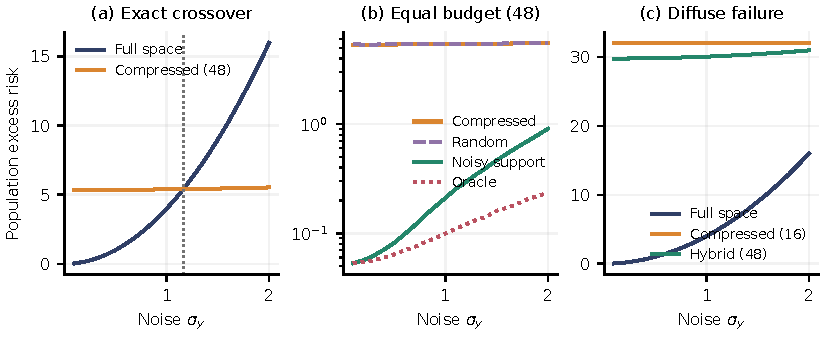
\includegraphics[width=\linewidth]{figures/sequence_summary.pdf}
 \caption{\textbf{Sequence-model tests.} (a) Full-space and compressed risk cross near the fixed-instance prediction $\sigma_y^\star\approx1.16$ (dashed). (b) At equal budget $B=48$, informed supports improve on compression; random support tracks it. (c) A dense target defeats both compression ($d=16$) and the larger hybrid ($d+K=48$) throughout the tested range. This last panel tests failure, not equal-budget superiority. Each target and its projections are fixed across the 200 noise trials and all noise levels; full decompositions are in Appendix~\ref{app:mechanism}.}
 \label{main:fig_sequence}
\end{figure}

The observed crossover agrees with the realized residual-energy threshold, rather than requiring an average over tasks. At matched budgets, random support approximately ties pure compression, while informed supports recover much more bias. The noisy support separates from the oracle as noise grows, exposing the cost excluded by the idealized independence assumption. In the diffuse regime the compressed bias floor is about $32$, above full-space LoRA across the tested range, and sparse correction recovers little. The original $d=16$ versus $d+K=48$ comparison and all decompositions remain in Appendix~\ref{sec:synthetic}; they illustrate bias recovery but are not evidence for equal-budget superiority.

\subsection{From the sequence model to a Transformer}
\label{main:transformer}
We pretrain and freeze a Transformer block of width 64 and sequence length 32, then plant query/value weight updates and fit noisy teacher outputs with AdamW. Compression and routing act in the identifiable $8192$-dimensional weight-update space, rather than the bilinear LoRA-factor coordinates. We compare rank-4 LoRA (1024 parameters), compressed-only adaptation ($B=128$), and hybrids ($d=K=64$), together with full updates and oracle/random supports. Thus this is a nonlinear bridge experiment, not an identical parameterization to every real-model run. We report excess prediction MSE, without the sequence model's factor $1/2$. The concentrated and diffuse teachers have functional displacements of $10\%$ and $100\%$, respectively; they vary magnitude as well as concentration. Appendix~\ref{sec:transformer_synthetic} specifies the construction and controls.

\begin{figure}[t]
 \centering
 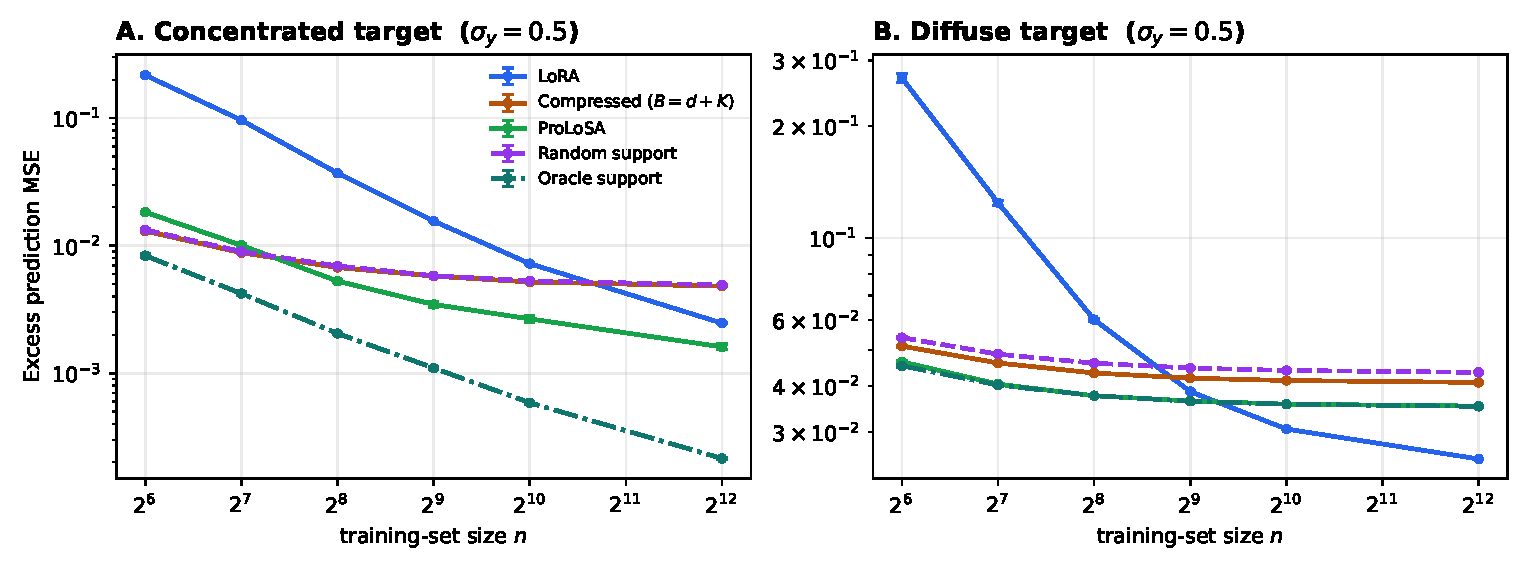
\includegraphics[width=\linewidth]{transformer_risk_vs_n.pdf}
 \caption{\textbf{Transformer teacher--student prediction MSE versus sample size.} Concentrated and diffuse targets, $\sigma_y=0.5$; mean $\pm$ s.e. over 20 training seeds for each fixed teacher. LoRA overtakes compression with more data. Sparse correction helps for concentrated residuals but little for diffuse residuals, even with oracle support. Compressed-only and all hybrids share budget 128. Additional noise levels and function-space decompositions are in Appendix~\ref{sec:transformer_synthetic}.}
 \label{main:fig_transformer}
\end{figure}

At $\sigma_y=0.5$, LoRA crosses below matched-budget compression around $n=2^9$--$2^{10}$ for the diffuse target and $n=2^{11}$ for the concentrated target (Figure~\ref{main:fig_transformer}). Higher noise shifts the crossover toward larger $n$. Noiseless large-sample fits show compressed approximation floors of $0.0047$ and $0.041$, respectively; oracle correction removes $99\%$ of the concentrated floor but only $13\%$ of the diffuse floor. Within each fixed teacher, function-space decompositions show the transition from high variance to a compressed bias floor; the two teachers are evaluated separately.

The finite-training deviations are also informative. At $n=4096$, $\sigma_y=1$, ProLoSA improves concentrated-target risk from $0.0052$ to $0.0030$, but at $n=64$, $\sigma_y=1.5$, noisy warmup selection worsens it from $0.066$ to $0.105$. Random hybrids do not outperform equal-budget compression and can be slightly worse under anisotropic curvature. These observations support residual recovery while delimiting the idealized variance equality in Proposition~\ref{prop:matched_budget}.

\subsection{Mechanism tests in real fine-tuning}
\label{main:real}
We next examine RoBERTa-large with rank-4 LoRA as a full-factor-space baseline and matched trainable budgets for Uni-LoRA and ProLoSA. Each comparison shares data subsets and evaluation sets; settings and full results are in Appendix~\ref{sec:real_model_validation}. We use dev loss for sample-size scaling, predictive probabilities for empirical decomposition, and diagonal empirical-Fisher weighting for residual diagnostics. These measurements address distinct parts of the argument and do not assume that raw factor norms measure functional error.

\begin{figure}[t]
 \centering
 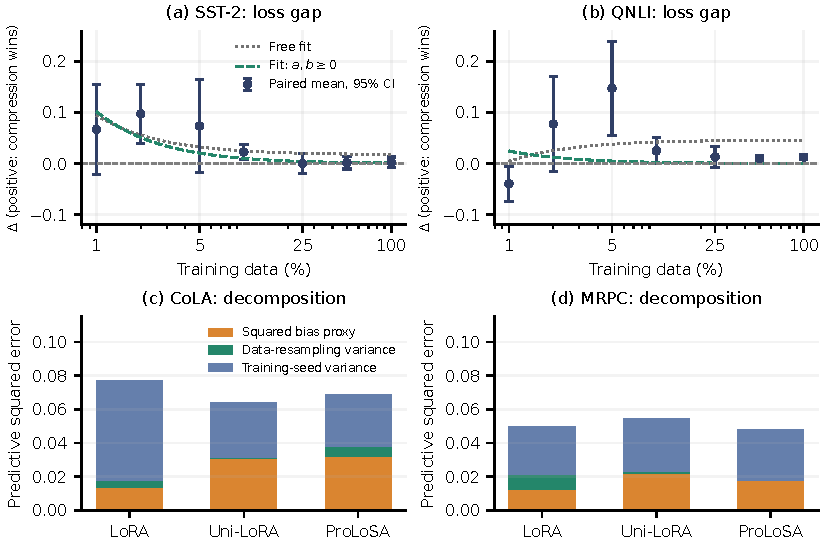
\includegraphics[width=\linewidth]{figures/real_mechanism.pdf}
 \caption{\textbf{Real-model evidence and limits.} Top: paired dev-loss gaps $\Delta=L_{\mathrm{LoRA}}-L_{\mathrm{Uni}}$ with pointwise 95\% $t$ intervals over five training seeds and free/constrained $a/n-b$ fits; positive favors compression. Subsets are fixed across seeds. Bottom: squared bias proxy, data-resampling variance, and training-seed variance, shown separately for five resamples and two seeds. The reference is a full-data LoRA ensemble; Table~\ref{tab:e3_reference} checks its sensitivity.}
 \label{main:fig_real}
\end{figure}

\paragraph{Sample-size scaling.}
We vary the training fraction from $1\%$ to $100\%$ with a fixed update-step budget and five paired training seeds, keeping the subset fixed at each fraction. SST-2's mean gap contracts from $0.067$ (95\% interval $[-0.021,0.155]$) to $0.002$ ($[-0.008,0.013]$). Fitting these paired means gives $\hat a=52.14$, $\hat b=-0.0171$, $R^2=0.485$; imposing $a,b\geq0$ places $b$ at zero and lowers $R^2$ to $0.358$. QNLI's free slope is negative ($\hat a=-43.90$, bootstrap interval $[-63.14,-29.14]$), and the auxiliary CoLA mean curve has $R^2=0.014$. These deviations challenge the local sample-size model under the present training protocol; they cannot be attributed solely to an unobserved crossover. Appendix~\ref{sec:real_model_validation} reports paired intervals, fit residuals, and uncertainty.

\paragraph{Predictive bias and variance.}
Five 80\% data resamples and two training seeds per resample separate data-resampling variability from within-resample variability, including initialization, optimization, and the compressed projection seed. On CoLA, Uni-LoRA lowers total variance from $0.0636$ to $0.0332$, but $88\%$ of this reduction comes from the training-seed component ($0.0593\to0.0326$), rather than the data component ($0.0043\to0.0006$). Thus the total decrease is not a measurement of $A_{\mathrm{var}}/n$. Squared bias relative to a full-data LoRA ensemble rises from $0.0136$ to $0.0309$. On MRPC, ProLoSA lowers Uni-LoRA's bias proxy from $0.0219$ to $0.0180$, with no increase in total variance; CoLA lacks this correction. Both bias orderings persist with rank-4-only, rank-64-only, and leave-one-reference-out ensembles. Finite-replicate corrections and clipping are detailed in the appendix.

\paragraph{Sparse recoverability.}
From an explicitly full-data, multi-seed LoRA target proxy, we form the Euclidean residual $q_E=(I-PP^\top)\Delta\theta$ and measure coordinate capture $\rho_{I,H}^2=\sum_{i\in I}\hat H_{ii}q_{E,i}^2/\sum_i\hat H_{ii}q_{E,i}^2$ using a diagonal empirical Fisher. Uniform size-$K$ support samples from all $D$ original coordinates, so its expected capture is $K/D$. The saved full-data SNIP supports show $16$--$194\times$ enrichment (Table~\ref{main:tab_recovery}), corroborated by 10,000 random supports per task. This coordinate diagnostic differs substantially from projection-bias recovery: on MRPC, capture is $18.04\%$ on $q_E$, $2.67\%$ on the $\hat H$-orthogonal residual, and joint refitting recovers $5.68\%$ of the latter's weighted energy. These are distinct proxies; none directly measures the unknown population quantity in Proposition~\ref{prop:matched_budget}. The support ablation below tests practical selection performance.

\begin{table}[t]
 \centering\small
 \caption{\textbf{Residual coordinate-energy capture.} Fisher-weighted fractions on the Euclidean residual of a full-data target proxy; enrichment uses $K/D$. Budgets, saved-support provenance, and the geometry comparison appear in Appendix~\ref{sec:real_model_validation}.}
 \label{main:tab_recovery}
 \begin{tabular}{lrrrr}
 \toprule
 Task & Oracle & SNIP & Reference & Enrichment \\
 \midrule
CoLA & 49.87\% & 7.91\% & 0.4883\% & $16.21\times$ \\
MRPC & 69.45\% & 18.04\% & 0.4883\% & $36.94\times$ \\
QNLI & 14.46\% & 3.12\% & 0.0407\% & $76.52\times$ \\
RTE & 33.74\% & 1.14\% & 0.0407\% & $27.98\times$ \\
STS-B & 51.91\% & 7.91\% & 0.0407\% & $194.13\times$ \\
 \bottomrule
 \end{tabular}
\end{table}

\section{Downstream Performance and Ablations}
\label{main:downstream}
Table~\ref{main:tab_performance} summarizes practical results; Appendix~\ref{app:downstream} contains all baselines, task-level scores, and hyperparameters. GLUE averages improve from $85.3$ to $85.5$ on RoBERTa-base and $88.3$ to $88.7$ on RoBERTa-large at the same compressed budget, while full LoRA remains stronger on the base-model average. Changing backbones changes representation quality and curvature as well as dimension, so this comparison is not a controlled variance test.

\begin{table}[t]
 \centering\small
 \caption{\textbf{Downstream summary.} Parameters are trainable counts. GLUE averages six tasks (five seeds); full task-level uncertainty and baseline provenance appear in Table~\ref{tab:glue}. Mathematical reasoning reports GSM8K / MATH (Gemma) or MATH500 (Llama); full comparisons are in Table~\ref{tab:math}. $^\dagger$VB-LoRA uses the original paper's parameter-count convention. Llama results use one seed and post-hoc compressed-configuration selection.}
 \label{main:tab_performance}
 \begin{tabular}{llrl}
 \toprule
 Backbone & Method & Parameters & Score(s) \\
 \midrule
 RoBERTa-base & LoRA & 0.295M & 86.6 \\
 & Uni-LoRA / ProLoSA & 0.023M & 85.3 / 85.5 \\
 RoBERTa-large & LoRA & 0.786M & 87.8 \\
 & VeRA & 0.061M & 87.8 \\
 & VB-LoRA & 0.162M$^\dagger$ & 88.2 \\
 & LoRA-XS & 0.025M & 87.9 \\
 & Uni-LoRA / ProLoSA & 0.023M & 88.3 / 88.7 \\
 \midrule
 Gemma-7B & LoRA & 200M & 74.90 / 31.28 \\
 & VeRA & 1.90M & 74.98 / 28.84 \\
 & FourierFT & 0.59M & 72.97 / 25.14 \\
 & Uni-LoRA & 0.52M & 75.59 / 28.94 \\
 & ProLoSA & 0.52M & 74.69 / 29.90 \\
 Llama-3.1-8B & LoRA ($r=64$) & 167.77M & 79.61 / 33.20 \\
 & Uni-LoRA & 1.05M & 75.44 / 26.20 \\
 & ProLoSA & 1.05M & 75.06 / 26.60 \\
 \bottomrule
 \end{tabular}
\end{table}

On mathematical reasoning, ProLoSA improves Gemma-7B's MATH score over Uni-LoRA by $0.96$ points but loses $0.90$ on GSM8K. Llama-3.1-8B similarly gains $0.40$ on MATH500 and loses $0.38$ on GSM8K; both compressed methods remain below rank-64 LoRA. These Llama results use seed 42, and the displayed compressed configurations maximize each method's two-benchmark mean among available runs at that budget: they are a post-hoc test-set summary, not an independently selected validation result (Appendix~\ref{app:llama31_math_sweep}). Each model is trained once on MetaMathQA and evaluated on both benchmarks, so their score differences cannot identify task-specific training-update energies. Instruction-tuning results are in Table~\ref{tab:instruction}; for example, LLaMA2-13B MT-Bench single-/multi-turn scores rise from $6.34/4.43$ to $6.57/4.72$ under a shared 1.0M budget.

\begin{table}[t]
 \centering\small
 \caption{\textbf{Vision transfer with ViT-B/16.} Final-model accuracy (\%, seed 42). All methods use rank 4 and train the classification head; adapter budgets exclude this shared head: LoRA has 147,456 parameters and both compressed methods have 24,600 ($d+K$ for ProLoSA). Parentheses give $d:K$. All four ratios are shown; no best-epoch or best-ratio selection is applied. Appendix~\ref{app:vit} gives exact budgets, settings, and the 72,000-budget sweep.}
 \label{tab:vit}
 \setlength{\tabcolsep}{5pt}
 % Generated from final_accuracy, seed 42; do not edit.
\begin{tabular}{lrrrrr}
\toprule
 & \multicolumn{3}{c}{1,000 training images} & \multicolumn{2}{c}{CIFAR-100} \\
\cmidrule(lr){2-4}\cmidrule(lr){5-6}
Method & CIFAR-100 & Food-101 & DTD & 5,000 & Full \\
\midrule
LoRA ($r=4$) & 86.91 & 79.50 & 73.14 & 89.87 & 92.41 \\
Uni-LoRA & 86.59 & 79.25 & 72.66 & 89.55 & 92.10 \\
ProLoSA ($2:1$) & 86.35 & 79.26 & 72.71 & 89.13 & 92.03 \\
ProLoSA ($4:1$) & 86.50 & 79.10 & 72.29 & 89.32 & 92.33 \\
ProLoSA ($8:1$) & 86.34 & 79.19 & 72.50 & 89.28 & 92.02 \\
ProLoSA ($12:1$) & 86.39 & 79.25 & 72.71 & 89.36 & 91.99 \\
\bottomrule
\end{tabular}

\end{table}

\paragraph{Vision transfer.}
Following Uni-LoRA's ViT experiments \citep{li2025unilora}, we evaluate ProLoSA on ViT-B/16 with shared data subsets and equal compressed-adapter budgets (Table~\ref{tab:vit}). At $d:K=4:1$, ProLoSA improves full-data CIFAR-100 accuracy from Uni-LoRA's $92.10$ to $92.33$, while LoRA reaches $92.41$. Gains are not consistent: all four allocations trail Uni-LoRA on CIFAR-100 with 1,000 and 5,000 images, and differences on Food-101 and DTD are small. These single-seed results extend the allocation study to vision without establishing a general advantage or a sample-size crossover; the training horizon also changes across data sizes.

\begin{table}[H]
 \centering\small
 \caption{\textbf{Equal-budget ablations}, $d+K=23040$. CoLA: Matthews correlation; MRPC: accuracy, mean $\pm$ std. Hybrid supports share $d=22320$, $K=720$. Full allocation and warmup sweeps are in Table~\ref{tab:ablation_budget_full}.}
 \label{main:tab_ablation}
 \begin{tabular}{lcc}
 \toprule
 Variant & CoLA & MRPC \\
 \midrule
 Compressed-only & $68.99\pm0.58$ & $90.93\pm0.00$ \\
 Sparse-only & $59.99\pm1.40$ & $84.89\pm0.83$ \\
 Random-support hybrid & $66.58\pm0.63$ & $90.28\pm0.61$ \\
 Gradient-support hybrid & $67.95\pm0.59$ & $90.03\pm0.31$ \\
 SNIP-support hybrid & $69.62\pm1.84$ & $91.69\pm0.40$ \\
 \bottomrule
 \end{tabular}
\end{table}

At a fixed total budget, SNIP support outperforms random and accumulated-gradient supports on both ablation tasks (Table~\ref{main:tab_ablation}); pure sparsity performs substantially worse. Random support also trails pure compression in the real network, unlike the idealized isotropic tie. The evidence favors informed residual allocation while retaining the practical effects of curvature, conditioning, and selection noise.

\section{Discussion and Conclusion}
\label{sec:conclusion}
This work develops a bias--variance explanation of compressed LoRA: its statistical advantage is governed by the balance between removed estimation variance and excluded task signal. The resulting conditions connect subspace geometry, noise, and sample size to beneficial and harmful compression, and motivate ProLoSA as a correction for recoverable projection bias under a fixed budget. Controlled and real-model experiments examine both the explanation and its design consequence. The exact thresholds belong to the sequence model; real-task sweeps do not establish a reliable crossover, and optimization effects or noisy support selection can alter the trade-off. These boundaries specify where further validation and theory are needed.


\clearpage
\section*{Reproducibility Statement}
\label{sec:repro_stmt}
Complete derivations and proofs are in Appendix~\ref{app:theory}; projection construction, support selection, and the training algorithm are in Appendix~\ref{app:method_details}. Appendix~\ref{app:mechanism} documents all mechanism experiments and their full results. Appendix~\ref{app:downstream} provides downstream configurations, task-level results, and ablations. All experiments use publicly available models and datasets. The summary figures are generated from the existing experiment CSVs and the reported tables by \texttt{figures/make\_summary\_figures.py}.

\section*{Ethics Statement}
This work studies statistical mechanisms of parameter-efficient fine-tuning using public models and benchmarks. It involves no human subjects, private data, or personally identifiable information. We do not foresee ethical concerns beyond those generally associated with fine-tuning large language models.

\section*{The Use of Large Language Models}
\label{app:llm_usage}
Large language models were used as writing-assistance tools, including polishing and reorganizing the exposition. The authors take responsibility for verifying all research claims, theoretical results, experimental descriptions, and empirical findings, and for the entire content of this paper.

\bibliography{iclr2027_conference}
\bibliographystyle{iclr2027_conference}
\clearpage
\appendix
\section{Extended Theory and Proofs}
\label{app:theory}
\subsection{Extended Related Work}
\label{app:related}

\paragraph{LoRA and structured parameter-efficient adaptation.}
LoRA \citep{hu2022lora} represents weight updates through low-rank factors; AdaLoRA and DoRA refine allocation and parameterization \citep{zhang2023adalora,liu2024dora}. Tied-LoRA, VeRA, NOLA, PRoLoRA, VB-LoRA, and LoRA-XS introduce sharing, frozen bases, or other structural restrictions \citep{renduchintala2024tied,kopiczko2024vera,koohpayegani2024nola,wang2024prolora,li2024vb,balazy2025lora}. Together with Uni-LoRA and FourierFT \citep{li2025unilora,gao2024fourierft}, these works motivate compact adaptation through representation efficiency and subspace design, including isometric reconstruction in Uni-LoRA and SVD-based gradient approximation in LoRA-XS. They do not develop a detailed bias--variance comparison of compression's generalization benefit over standard LoRA. Our fixed reconstruction directly describes the Uni-LoRA branch studied here; transferring its risk conditions to other parameterizations requires specifying their estimation space and verifying the assumptions.

\paragraph{Intrinsic dimension and the statistical comparison.}
Low intrinsic dimension provides evidence that effective adaptation can use few degrees of freedom. Aghajanyan et al.\ \citep{aghajanyan2021intrinsic} additionally connect intrinsic dimension to compression-based generalization bounds. Thus the existing perspective includes statistical theory as well as representation evidence. Our focus is the relative population risk of compressed and full-space estimators: a restriction can improve estimation by removing noisy directions, or harm it by excluding task signal. The projection bias and retained variance make this comparison depend on the chosen subspace and data regime. Isometry within a represented subspace does not determine the energy outside it, and dimensionality alone does not specify either term under anisotropic curvature. These distinctions motivate our success/failure conditions and the corresponding measurements.

\paragraph{Recent LoRA theory and optimization.}
Zeng and Lee \citep{zeng2024expressive} characterize LoRA's expressive power. Liu et al.\ \citep{liu2025landscape} compare optimization landscapes of LoRA, GaLore, and full-rank methods. LoRA-Pro derives gradient adjustments from a gradient-matching objective \citep{wang2025lorapro}; LoRA-RITE studies factorization invariance and constructs an adaptive preconditioner \citep{yen2025lorarite}; Stable-LoRA links feature-learning stability to an early weight-shrinkage strategy \citep{wu2026stablelora}. These works connect concrete adaptation properties to algorithm design. We analyze the risk trade-off introduced by further compression of LoRA parameters, and derive sparse residual correction as a consequence of that statistical account. Optimization theory remains complementary: the optimization variance measured in our real-model study need not follow the asymptotic statistical-variance law.

\paragraph{Sparse and hybrid adaptation.}
SparseAdapter \citep{he2022sparseadapter} prunes adapter parameters, SIFT and SpIEL optimize sparse subsets of model updates \citep{song2024sparse,ansell2024scaling}, and RoSA combines low-rank and sparse updates \citep{nikdan2024rosa}. ProLoSA augments a globally compressed LoRA-factor vector with selected residual coordinates. Its design criterion compares recovered projection bias against the opportunity cost of allocating a fixed budget to these coordinates. This provides a specific statistical motivation for the hybrid, with the reliability of practical support selection assessed separately by the experiments.

\paragraph{Subspace restriction and statistical regularization.}
The mathematical tools build on shrinkage, principal-component regression, and compressed least-squares analysis \citep{james1961estimation,hastie2009elements,maillard2009compressed,kaban2014new,thanei2017random}. We use projection-risk calculations to connect compression geometry to the statistical comparison of adaptation estimators. The sequence model isolates the fixed-task residual threshold; the local extension links it to curvature and sample size; the matched-budget analysis identifies the cost and benefit of recovering excluded directions. Their empirical relevance is evaluated at distinct levels of idealization, rather than inferred from low parameter count alone.

\subsection{When and Why Compression Makes LoRA Better}
\label{sec:theory}

We view compressed LoRA as restricted estimation in the full LoRA parameter space, decompose its excess risk into projection bias and estimation variance (Appendix~\ref{sec:bias_variance}), and specialize the resulting crossover condition into an interpretable energy--noise condition that characterizes exactly when compression helps and when it must fail (Appendix~\ref{sec:when_fails}).

\subsubsection{A Bias--Variance View of Compressed LoRA}
\label{sec:bias_variance}

Let $\theta_D\in\mathbb{R}^D$ collect the vectorized trainable LoRA factors across all adapted layers.
Whereas standard LoRA optimizes these $D$ entries directly, compressed variants learn a latent vector $\theta_d\in\mathbb{R}^d$, with $d\ll D$, from which they reconstruct the full parameter vector.
We study the following linear form, which provides a common abstraction of such parameter sharing:
\begin{equation}
\theta_D=P\theta_d,
\label{eq:compressed_lora_projection}
\end{equation}
where $P\in\mathbb{R}^{D\times d}$ is a fixed reconstruction matrix.
Standard LoRA is recovered by setting $d=D$ and $P=I_D$.
Equation~\eqref{eq:compressed_lora_projection} also captures the Uni-LoRA-style parameterization \citep{li2025unilora} used by our compressed branch; its specific construction is given in Appendix~\ref{sec:prolosa_parameterization}.
For notational simplicity, below $\theta\in\mathbb{R}^D$ denotes a generic value of the full LoRA vector $\theta_D$.

Let $f(x;\theta)$ denote the prediction of the frozen backbone equipped with LoRA parameters $\theta$, and let $\ell(f(x;\theta),y)$ denote the per-example loss between that prediction and its target $y$ (e.g., cross-entropy for classification).
Following the standard risk-minimization framework \citep{vapnik1998statistical,hastie2009elements,vanderVaart1998asymptotic}, we define the population and empirical risks as
\begin{equation}
R(\theta)
:=
\mathbb{E}_{(x,y)\sim\mathcal{D}}
\!\left[\ell(f(x;\theta),y)\right],
\qquad
\widehat R_n(\theta)
:=
\frac{1}{n}\sum_{i=1}^{n}
\ell(f(x_i;\theta),y_i),
\label{eq:population_empirical_risk}
\end{equation}
where $\mathcal{D}$ is the downstream data distribution and $\{(x_i,y_i)\}_{i=1}^n$ are $n$ i.i.d.\ samples from $\mathcal{D}$.
We write
$\theta^\star=\arg\min_{\theta\in\mathbb{R}^D}R(\theta)$
for the full-space population optimum and
$\hat{\theta}_L=\arg\min_{\theta\in\mathbb{R}^D}\widehat R_n(\theta)$
for the empirical minimizer obtained by standard LoRA.
For a fixed data distribution $\mathcal D$, $\theta^\star$ is a fixed population optimum (choosing one representative if it is nonunique); randomness across training samples belongs to $\hat\theta_L$, not to $\theta^\star$.

Assuming that $R$ is twice differentiable near $\theta^\star$, a second-order expansion gives
\begin{equation}
R(\theta)
\approx
R(\theta^\star)
+
\frac{1}{2}
(\theta-\theta^\star)^\top
H
(\theta-\theta^\star),
\label{eq:local_quadratic}
\end{equation}
where $H:=\nabla^2R(\theta^\star)\succeq 0$ is the local curvature at the optimum; the first-order term vanishes by stationarity.
This approximation describes only a neighborhood of $\theta^\star$ and does not require $R$ to be globally convex.

To isolate the variance induced by estimating LoRA parameters from finite data, we first consider the locally centered regime
$\mathbb{E}[\hat{\theta}_L]=\theta^\star$ and write
\begin{equation}
\hat{\theta}_L=\theta^\star+\xi_L,
\label{eq:lora_centered_decomp}
\end{equation}
where $\xi_L:=\hat{\theta}_L-\mathbb{E}[\hat{\theta}_L]$ is the centered estimation error.
Thus, $\mathbb{E}[\xi_L]=0$ and $\Sigma_L:=\operatorname{Cov}(\xi_L)$.
Substitution into Eq.~\eqref{eq:local_quadratic}, followed by expectation over the training sample, yields
\begin{equation}
\mathbb{E}[R(\hat{\theta}_L)]-R(\theta^\star)
\approx
\frac{1}{2}\mathrm{tr}(H\Sigma_L).
\label{eq:lora_excess_risk}
\end{equation}
Standard LoRA incurs no subspace-approximation bias, but estimating all $D$ coordinates may produce substantial variance.
Appendix~\ref{app:general_bias_variance} relaxes the centering assumption and retains finite-sample and optimization bias.

A compressed parameterization instead restricts optimization to
$\mathcal{S}_U:=\mathrm{col}(P)\subseteq\mathbb{R}^D$.
Define
$\theta^\star_U=\arg\min_{\theta\in\mathcal{S}_U}R(\theta)$
as the restricted population optimum and
$\hat{\theta}_U=\arg\min_{\theta\in\mathcal{S}_U}\widehat R_n(\theta)$
as its empirical counterpart.
Under the local quadratic model, $\theta^\star_U$ is the $H$-weighted projection of $\theta^\star$ onto $\mathcal{S}_U$.
Let $z^\star_U,\hat{z}_U\in\mathbb{R}^d$ be latent representations satisfying
$\theta^\star_U=Pz^\star_U$ and $\hat{\theta}_U=P\hat{z}_U$.
Under the analogous centered condition $\mathbb{E}[\hat{z}_U]=z^\star_U$, we write
\begin{equation}
\hat{\theta}_U=\theta^\star_U+P\zeta,
\label{eq:compressed_centered_decomp}
\end{equation}
where $\zeta:=\hat{z}_U-\mathbb{E}[\hat{z}_U]$ is the centered latent error.
Here, $\mathbb{E}[\zeta]=0$ and $\Sigma_z:=\operatorname{Cov}(\zeta)$.
Applying the same calculation as above gives
\begin{equation}
\mathbb{E}[R(\hat{\theta}_{U})]-R(\theta^\star)
\approx
\underbrace{
\frac{1}{2}
(\theta^\star_U-\theta^\star)^\top
H
(\theta^\star_U-\theta^\star)
}_{\text{projection bias}}
+
\underbrace{
\frac{1}{2}
\mathrm{tr}(HP\Sigma_zP^\top)
}_{\text{estimation variance}} .
\label{eq:compressed_excess_risk}
\end{equation}
The two terms expose the central trade-off: compression reduces estimation variance by restricting the fitted directions, but generally introduces bias by excluding part of the full-space optimum.
Comparing Eqs.~\eqref{eq:lora_excess_risk} and~\eqref{eq:compressed_excess_risk}, compressed LoRA has lower expected excess risk precisely when
\begin{equation}
(\theta^\star_U-\theta^\star)^\top
H
(\theta^\star_U-\theta^\star)
+
\mathrm{tr}(HP\Sigma_zP^\top)
<
\mathrm{tr}(H\Sigma_L).
\label{eq:compression_condition}
\end{equation}
Thus, a smaller parameter space need not weaken generalization: the restriction is beneficial whenever the variance removed from excluded directions exceeds the projection bias introduced by excluding them.

\subsubsection{When Compression Helps, and When It Must Fail}
\label{sec:when_fails}

Although Condition~\eqref{eq:compression_condition} applies to general local curvature and estimator covariance, these quantities obscure the dependence of the trade-off on target energy and estimation noise.
We first specialize to an isotropic sequence model for a \emph{fixed} task, matching the repeated-noise protocol of Appendix~\ref{sec:synthetic}.
Fix $\theta^\star\in\mathbb R^D$ and $P\in\mathbb R^{D\times d}$ with $P^\top P=I_d$ and $0<d<D$.
Observe $y=\theta^\star+\sigma_{\mathrm{eff}}\epsilon$, where $\epsilon\sim\mathcal N(0,I_D)$, and let
$R(\theta)-R(\theta^\star)=\frac12\|\theta-\theta^\star\|_2^2$ ($H=I$).
The least-squares estimators are $\hat\theta_L=y$ and $\hat\theta_U=PP^\top y$.
Averaging over observation noise alone gives
\begin{equation}
\mathbb E_\epsilon\!\left[R(\hat\theta_U)-R(\theta^\star)\mid\theta^\star,P\right]
=
\underbrace{\frac12\|(I-PP^\top)\theta^\star\|_2^2}_{\text{fixed projection bias}}
+
\underbrace{\frac12d\sigma_{\mathrm{eff}}^2}_{\text{estimation variance}},
\label{eq:conditional_compressed_risk}
\end{equation}
while the full-space risk is $\frac12D\sigma_{\mathrm{eff}}^2$.
Thus, for this fixed instance, compression helps if and only if
\begin{equation}
\hat v_\perp<\sigma_{\mathrm{eff}}^2,
\qquad
\hat v_\perp:=\frac{\|(I-PP^\top)\theta^\star\|_2^2}{D-d}.
\label{eq:fixed_energy_noise_condition}
\end{equation}
Here $\hat v_\perp$ is a deterministic realized residual energy per excluded dimension; no distributional assumption on $\theta^\star$ is needed.

\paragraph{Optional averaging over generated problem instances.}
To summarize an ensemble of tasks, introduce a separate random target $\Theta^\star\sim\mathcal Q$, of which the fixed optimum $\theta^\star$ is one realization.
Assume
$\mathbb E_{\mathcal Q}[\Theta^\star]=0$ and
$\mathbb E_{\mathcal Q}[\Theta^\star{\Theta^\star}^\top]=vI_D$, where
$v:=D^{-1}\mathbb E_{\mathcal Q}\|\Theta^\star\|_2^2$.
This is a \emph{problem-generation assumption}, not an expectation over repeated datasets from one task: for those repeats,
$\mathbb E_\epsilon[\theta^\star{\theta^\star}^\top\mid\theta^\star,P]=\theta^\star{\theta^\star}^\top$.
Let $P$ be fixed or drawn independently of $\Theta^\star$, with observation noise independent of both.
Write $\mathbb E_{\mathrm{ens}}$ for the additional average over generated targets and, if random, projections, as well as observation noise; each risk is evaluated for its corresponding realized task.

\begin{quote}\textbf{Ensemble energy--noise condition (restated).}

Under the additional isotropic target law above, averaging the fixed-instance risks yields
\begin{equation}
\begin{aligned}
\mathbb E_{\mathrm{ens}}[R(\hat\theta_L)-R(\theta^\star)]&=\tfrac12D\sigma_{\mathrm{eff}}^2,\\
\mathbb E_{\mathrm{ens}}[R(\hat\theta_U)-R(\theta^\star)]&=
\underbrace{\tfrac12(D-d)v}_{\text{mean projection bias}}
+\underbrace{\tfrac12d\sigma_{\mathrm{eff}}^2}_{\text{estimation variance}}.
\end{aligned}
\label{eq:energy_noise_risks}
\end{equation}
Consequently, compression reduces the \emph{ensemble-average} excess risk if and only if
\begin{equation}
v<\sigma_{\mathrm{eff}}^2.
\label{eq:energy_noise_condition}
\end{equation}
\end{quote}
Appendix~\ref{app:energy_noise_condition} proves both the fixed-instance and ensemble results.
Under $\mathcal Q$, $\mathbb E_{\mathrm{ens}}[\hat v_\perp]=v$.
Any target-independent orthonormal $P$, including normalized one-hot and random orthonormal constructions, has the same ensemble risk at a given $d$; their biases need not agree for a fixed target.
The synthetic noise trials estimate Eq.~\eqref{eq:conditional_compressed_risk}, rather than the ensemble average in Eq.~\eqref{eq:energy_noise_risks}.

\paragraph{Remark (parameterization dependence of $v$).}
The scalar $v=D^{-1}\mathbb E_{\mathcal Q}\|\Theta^\star\|_2^2$ is defined in the chosen LoRA-factor parameterization and is \emph{not} invariant to equivalent factorizations of the same effective update: the gauge freedom $(A_\ell,B_\ell)\mapsto(c\,A_\ell,B_\ell/c)$ leaves $\Delta W_\ell=B_\ell A_\ell$ unchanged while rescaling the factor-space norm arbitrarily. All statements involving $v$ are therefore comparisons made \emph{within a fixed parameterization, initialization scale, and training protocol}, and we use $v<\sigma_{\mathrm{eff}}^2$ only as the interpretable specialization of the general condition~\eqref{eq:compression_condition} to the isotropic model. In real networks, the parameterization-appropriate quantity is the curvature-weighted projection bias $B_{\mathrm{proj}}=\frac{1}{2}(\theta^\star_U-\theta^\star)^\top H(\theta^\star_U-\theta^\star)$ of Eq.~\eqref{eq:compressed_excess_risk}, which weights each direction by its functional relevance; $B_{\mathrm{proj}}$ (estimated with a Fisher approximation of $H$) is the primary object measured in the Transformer experiment of Appendix~\ref{sec:transformer_synthetic} and the downstream experiments of Appendix~\ref{sec:real_model_validation}.

Proposition~1 is an exact result for this isotropic sequence model, not a universal characterization of neural-network fine-tuning; it provides a controlled baseline for interpreting the more general condition in Eq.~\eqref{eq:compression_condition}.
Within this model, it has three consequences.
(i)~\emph{Why compression can work for fine-tuning:} for a target ensemble with modest average energy $v$, limited data can induce comparatively large $\sigma_{\mathrm{eff}}^2$, placing the average problem in the variance-dominated regime $v<\sigma_{\mathrm{eff}}^2$; for a fixed task, the corresponding comparison uses $\hat v_\perp$. Evidence that downstream adaptation often has low intrinsic dimension \citep{aghajanyan2021intrinsic} supports the broader premise that strong restrictions can be effective, but does not by itself imply that either energy quantity is small.
(ii)~\emph{Why compression can fail when the required update is large:} for a dense, high-energy target ensemble---modeling tasks that demand large parameter changes rather than small downstream corrections---the average condition reverses to $v>\sigma_{\mathrm{eff}}^2$. For a fixed task, compression is worse whenever $\hat v_\perp>\sigma_{\mathrm{eff}}^2$, because its realized projection-bias floor exceeds the variance removed. Compressed parameterizations are therefore poorly suited to adaptation problems whose updates are large in magnitude and diffuse across coordinates.
(iii)~\emph{Recoverability depends on the energy profile:} if the off-subspace energy is heavy-tailed---a few coordinates carry most of it, as is characteristic of fine-tuning updates---a budget of $K\ll D$ residual directions recovers most of the bias, motivating Appendix~\ref{sec:method}; if it is diffuse, as for dense Gaussian targets, the best $K$ coordinates capture only an $O\!\big((K/D)\log(D/K)\big)$ fraction (Appendix~\ref{app:energy_noise_condition}), and no small sparse correction can rescue compression.
Both predictions are tested in Appendix~\ref{sec:synthetic}.

\subsubsection{From the Bias--Variance Decomposition to Testable Downstream Predictions}
\label{sec:testable_predictions}

We now translate Eq.~\eqref{eq:compressed_excess_risk} into sample-size predictions.
For one observation $(x,y)\sim\mathcal D$, define the per-sample score
\begin{equation}
\psi(x,y;\theta)
:=
\nabla_\theta \ell(f(x;\theta),y)
\in\mathbb R^D,
\qquad
G
:=
\operatorname{Cov}_{(x,y)\sim\mathcal D}
\!\left[\psi(x,y;\theta^\star)\right].
\label{eq:score_covariance}
\end{equation}
Thus, $G\succeq0$ is the covariance of the stochastic loss gradient at the full-space population optimum; it measures gradient noise across examples.
It is distinct from $H=\nabla^2R(\theta^\star)$, which measures the local curvature of the mean loss.

Under the regularity conditions for a fixed-dimensional M-estimator---i.i.d.\ sampling, a locally unique identifiable optimum, finite second moments of $\psi$, and consistent empirical minimization---the M-estimator central limit theorem gives the sandwich covariance \citep{vanderVaart1998asymptotic,white1982maximum}
\begin{equation}
\sqrt n\,(\hat\theta_L-\theta^\star)
\ \rightsquigarrow\
\mathcal N\!\left(0,H^\dagger G H^\dagger\right).
\label{eq:lora_m_estimator_clt}
\end{equation}
Here $\rightsquigarrow$ denotes convergence in distribution and ${}^\dagger$ the Moore--Penrose pseudoinverse.
The pseudoinverse is shorthand for restricting the calculation to the locally identifiable tangent space: bilinear LoRA has gauge directions along which $H$ is singular, whereas $H$ is assumed positive definite after those directions are quotiented out.

The central limit theorem is used to obtain Eq.~\eqref{eq:lora_m_estimator_clt}; it does \emph{not} imply $G=H$.
That equality is the information-matrix identity and holds, under additional regularity conditions, for a correctly specified negative-log-likelihood model.
We do not require it here, so the general sandwich form retains both matrices.

For the compressed estimator, the per-sample latent score is $P^\top\psi(x,y;Pz)$.
To obtain a tractable two-parameter prediction, we use the same local quadratic neighborhood as Appendix~\ref{sec:bias_variance}: the curvature and score covariance at $\theta^\star_U$ are approximated by those at $\theta^\star$.
The latent Hessian and score covariance are then $P^\top HP$ and $P^\top GP$, respectively, and
\begin{equation}
\Sigma_L
\approx
\frac{1}{n}H^\dagger G H^\dagger,
\qquad
\Sigma_z
\approx
\frac{1}{n}
(P^\top HP)^\dagger
P^\top GP
(P^\top HP)^\dagger,
\label{eq:local_asymptotic_covariances}
\end{equation}
where $\Sigma_L=\operatorname{Cov}(\hat\theta_L)$ and $\Sigma_z=\operatorname{Cov}(\hat z_U)$ are the estimator covariances introduced in Appendix~\ref{sec:bias_variance}.
If $\theta^\star_U$ is not close enough to $\theta^\star$ for this shared-local approximation, its own Hessian and score covariance must replace $P^\top HP$ and $P^\top GP$, and the simple expression below need not hold.
Moreover, Eq.~\eqref{eq:local_asymptotic_covariances} is a large-$n$, fixed-dimensional approximation for empirical risk minimizers.
Early stopping, SGD's implicit regularization, and regimes with parameter dimension comparable to or larger than $n$ can alter the covariance, so the resulting $1/n$ law is a prediction to be tested rather than an exact description of practical fine-tuning.

Substituting Eq.~\eqref{eq:local_asymptotic_covariances} into Eqs.~\eqref{eq:lora_excess_risk} and~\eqref{eq:compressed_excess_risk} gives the \emph{compression advantage}
\begin{equation}
\Delta(n)
:=
\mathbb{E}\big[R(\hat{\theta}_L)\big]-\mathbb{E}\big[R(\hat{\theta}_U)\big]
\approx
\frac{A_{\mathrm{var}}}{n}-B_{\mathrm{proj}},
\label{eq:risk_gap_n}
\end{equation}
where
\begin{equation}
A_{\mathrm{var}}
:=
\frac{1}{2}
\left[
\mathrm{tr}(H^\dagger G)
-
\mathrm{tr}\!\left((P^\top HP)^\dagger P^\top GP\right)
\right]
\ge 0,
\qquad
B_{\mathrm{proj}}
:=
\frac{1}{2}
(\theta^\star_U-\theta^\star)^\top
H
(\theta^\star_U-\theta^\star).
\label{eq:variance_projection_coefficients}
\end{equation}
Here $A_{\mathrm{var}}$ is the per-sample estimation-variance coefficient removed by restricting optimization to $\mathcal S_U=\operatorname{col}(P)$, and $B_{\mathrm{proj}}$ is the $n$-independent curvature-weighted projection bias.
Under the shared $H,G$ approximation, $A_{\mathrm{var}}\ge0$: in identifiable coordinates the second trace integrates the positive-semidefinite matrix $H^{-1/2}GH^{-1/2}$ over the whitened compressed subspace, whereas the first integrates it over the full tangent space.

When $A_{\mathrm{var}}>0$ and $B_{\mathrm{proj}}>0$, define the crossover $n^\star:=A_{\mathrm{var}}/B_{\mathrm{proj}}$; Eq.~\eqref{eq:risk_gap_n} then predicts lower risk for compression when $n<n^\star$.
If $B_{\mathrm{proj}}=0$, the model instead predicts a nonnegative compression advantage for every finite $n$ (formally, $n^\star=\infty$); if $A_{\mathrm{var}}=0<B_{\mathrm{proj}}$, compression cannot help.
In the fixed-instance isotropic model, $A_{\mathrm{var}}/n=\frac12(D-d)\sigma_{\mathrm{eff}}^2$ and $B_{\mathrm{proj}}=\frac12(D-d)\hat v_\perp$, recovering Eq.~\eqref{eq:fixed_energy_noise_condition}. Only after averaging over the target law does $\mathbb E_{\mathrm{ens}}[B_{\mathrm{proj}}]=\frac12(D-d)v$ recover Proposition~\ref{prop:energy_noise}.
Equation~\eqref{eq:risk_gap_n} now yields three direct comparative statics, obtained by varying $n$, $G$, and $P$, respectively.

\textbf{(P1) Sample-size scaling.}
Holding the task, data distribution, optimization protocol, and subspace fixed, $\Delta$ should be approximately affine in $1/n$, with slope $A_{\mathrm{var}}\ge0$ and intercept $-B_{\mathrm{proj}}\le0$.
A sign change is expected only when both coefficients are strictly positive and the corresponding $n^\star$ lies in the observed range.

\textbf{(P2) Noise scaling.}
Consider a label perturbation with standard deviation $\tau$ that preserves the population optimum but increases the score covariance $G$---for example, independent zero-mean additive label noise under squared loss.
More precisely, suppose $G(\tau)=G_0+\tau^2G_{\mathrm{noise}}$ with $G_{\mathrm{noise}}\succeq0$, while $H$ and $\theta^\star$ remain fixed.
Because $A_{\mathrm{var}}$ is linear in $G$, Eq.~\eqref{eq:risk_gap_n} gives
\begin{equation}
\Delta(\tau)
\approx
\Delta(0)+c_1\tau^2,
\qquad
c_1
=
\frac{1}{2n}
\left[
\mathrm{tr}(H^\dagger G_{\mathrm{noise}})
-
\mathrm{tr}\!\left(
(P^\top HP)^\dagger P^\top G_{\mathrm{noise}}P
\right)
\right]
\ge0.
\label{eq:noise_scaling_prediction}
\end{equation}
The inequality is strict when the added gradient noise has a nonzero component in directions excluded by the compressed subspace.
This statement does not apply automatically to label flipping or arbitrary losses, for which the perturbation may move $\theta^\star$ and change both terms.

\textbf{(P3) Subspace alignment.}
For two equal-dimensional projections $P_1$ and $P_2$, Eq.~\eqref{eq:risk_gap_n} gives
\begin{equation}
\Delta(P_1)-\Delta(P_2)
\approx
\frac{A_{\mathrm{var}}(P_1)-A_{\mathrm{var}}(P_2)}{n}
-
\left[
B_{\mathrm{proj}}(P_1)-B_{\mathrm{proj}}(P_2)
\right].
\label{eq:subspace_alignment_prediction}
\end{equation}
Thus, if the removed-variance coefficients are equal or tightly controlled, the better-aligned projection---the one with smaller $B_{\mathrm{proj}}$---has the larger compression advantage.
Equal dimension alone is insufficient in an anisotropic problem because changing $P$ generally changes both terms.

P1--P3 are therefore not independent heuristics: they probe the sample size, noise covariance, and subspace geometry in the same risk-gap decomposition.
They diagnose when pure compression should help, but do not specify how to reduce $B_{\mathrm{proj}}$ when the chosen subspace omits important directions.
Appendix~\ref{sec:sparse_bias} addresses that constructive question and derives the sparse-recoverability prediction P4 from a matched-budget comparison.


\subsection{Sparse Residual Correction under Matched Budgets}
\label{sec:sparse_bias}

Let $I=\{i_1,\ldots,i_K\}\subseteq\{1,\ldots,D\}$ be a sparse support of size $K$ with coordinate-selection matrix $E_I=[e_{i_1},\ldots,e_{i_K}]\in\mathbb{R}^{D\times K}$, so that the hybrid parameterization optimizes over $\mathrm{col}([P,E_I])$.
Adding $K$ sparse directions to a \emph{fixed} compressed space can never increase the best attainable approximation bias, since the feasible set only grows (Appendix~\ref{app:sparse_bias_reduction}); this nested comparison, however, spends $d+K$ parameters against $d$ and therefore does not describe our experiments, which match the \emph{total} budget.
The relevant question is: given a fixed budget $B$, is it better to spend all of it on a larger projected space, or to reserve $K$ coordinates for sparse correction?
The isotropic setting of Proposition~1 gives a sharp answer.

\begin{quote}\textbf{Matched-budget condition (restated).}

In the setting of Proposition~\ref{prop:energy_noise}, compare (a) a compressed-only parameterization with projection dimension $B$ and (b) a hybrid parameterization with projection dimension $d=B-K$ and a sparse support $\hat{I}$ of size $K$ selected independently of the estimation noise, with $\operatorname{rank}([P,E_{\hat{I}}])=B$.
Expectations in this proposition are ensemble averages as defined in Appendix~\ref{sec:when_fails}.
Both have the same expected estimation variance $\frac{1}{2}B\sigma_{\mathrm{eff}}^2$, and their expected excess risks differ only through the bias:
\begin{equation}
\mathbb E_{\mathrm{ens}}\big[R(\hat{\theta}_{\mathrm{hyb}})\big]
-
\mathbb E_{\mathrm{ens}}\big[R(\hat{\theta}_{U,B})\big]
=
\frac{1}{2}\Big(K\,v-\mathbb E_{\mathrm{ens}}\big[\mathcal{E}_K\big]\Big),
\label{eq:matched_budget_condition}
\end{equation}
Writing $q=(I-PP^\top)\theta^\star$, $A_{\hat I}=(I-PP^\top)E_{\hat I}$, and $\Pi_{A_{\hat I}}$ for the orthogonal projector onto $\operatorname{col}(A_{\hat I})$, the captured off-subspace energy is
$\mathcal E_K:=\|\Pi_{A_{\hat I}}q\|_2^2$.
Hence, under a matched budget, the hybrid parameterization wins if and only if the selected directions recover above-average residual energy, $\mathbb E_{\mathrm{ens}}[\mathcal{E}_K]>Kv$.
\end{quote}
The proof is given in Appendix~\ref{app:matched_budget}.
Let $P_B^\top P_B=I_B$ denote the budget-$B$ baseline projection. For fixed $\theta^\star,P,P_B$ and a fixed noise-independent support $I$ with $\operatorname{rank}([P,E_I])=B$, the corresponding risk difference is instead
\begin{equation}
\mathbb E_\epsilon\!\left[R(\hat\theta_{\mathrm{hyb}})-R(\hat\theta_{U,B})\mid\theta^\star,P,P_B,I\right]
=\frac12\left(\|q\|_2^2-\mathcal E_K-\|(I_D-P_BP_B^\top)\theta^\star\|_2^2\right).
\label{eq:fixed_matched_budget_condition}
\end{equation}
Thus, $Kv$ in Eq.~\eqref{eq:matched_budget_condition} is an ensemble-average opportunity cost, not the exact cost for a single realized target and pair of projections.

\textbf{(P4) Sparse recoverability.}
Unlike P1--P3, this prediction is a constructive consequence of Proposition~\ref{prop:matched_budget}, rather than a direct comparative static of Eq.~\eqref{eq:risk_gap_n}.
At a fixed total budget $B$, the hybrid's expected advantage over pure compression is
$\frac{1}{2}\big(\mathbb E_{\mathrm{ens}}[\mathcal E_K]-Kv\big)$.
It is therefore governed by the off-subspace energy recovered by the selected support, not by the total update norm: target-independent support gives no expected gain, while a support capturing above-average residual energy reduces projection bias without increasing the idealized variance term.
Experiment E5 in Appendix~\ref{sec:real_model_validation} tests this implication directly.

Proposition~\ref{prop:matched_budget} sharpens the design principle in two ways, both examined empirically.
First, \emph{uninformed sparsity provides no expected gain}: under the isotropic target model, any $B$-dimensional subspace selected independently of $\theta^\star$ has the same expected approximation error, so a random support captures exactly $\mathbb E_{\mathrm{ens}}[\mathcal{E}_K]=Kv$ and the random hybrid matches the $B$-dimensional compressed-only estimator in expectation (Corollary~\ref{cor:random_support} in Appendix~\ref{app:matched_budget}); the sequence-model experiment in Appendix~\ref{sec:synthetic} exhibits a near-tie for its single realized target, rather than directly estimating this ensemble equality.
The benefit of the hybrid parameterization must therefore come from \emph{data-dependent, target-informed support selection}, not from sparsity itself.
Second, \emph{informed selection on concentrated energy wins}: when the off-subspace energy is heavy-tailed, the top-$K$ coordinates identified during warmup carry far more than $Kv$ of energy, so reserving a small $K$ strictly reduces risk; when the energy is diffuse, the captured fraction of the bias floor is negligible and the hybrid cannot rescue compression, consistent with the failure regime of Appendix~\ref{sec:when_fails}.
Detailed derivations, including the general anisotropic decomposition and the risk-level condition for a fixed support, are provided in Appendices~\ref{app:general_bias_variance}--\ref{app:prolosa_bias_variance_condition}.

\paragraph{Remark (selection variance under data-dependent supports).}
Proposition~\ref{prop:matched_budget} isolates the idealized benefit of allocating budget to target-informed residual directions while assuming the support is selected independently of the estimation noise.
In practice, ProLoSA selects its support from warmup statistics computed on the \emph{same} training data used for estimation, which violates this independence: by the law of total covariance,
$\operatorname{Cov}(\hat\theta)=\mathbb E_{\hat I}\big[\operatorname{Cov}(\hat\theta\mid\hat I)\big]+\operatorname{Cov}_{\hat I}\big(\mathbb E[\hat\theta\mid\hat I]\big)$,
where the second term is an additional \emph{selection variance} induced by the noise-dependence of $\hat I$, and noisy scores can also inflate the apparent captured energy of the selected coordinates.
The hybrid therefore helps only when the captured bias reduction exceeds this extra variance.
This effect is directly visible in our experiments: in the sequence model, the noise-dependent support degrades gracefully relative to an oracle support as $\sigma_y$ grows (Appendix~\ref{sec:synthetic}), and in the Transformer experiment ProLoSA falls behind the matched-budget compressed baseline precisely in the small-$n$, high-noise corner where support selection is least reliable (Appendix~\ref{sec:transformer_synthetic}).


\subsection{General Bias--Variance Decomposition with Finite-Sample Bias}
\label{app:general_bias_variance}

The main text presents the locally centered case for clarity.
Here we provide the more general decomposition that explicitly includes finite-sample estimation bias, optimization bias, or deviations from the ideal local quadratic model.

For classical LoRA, let
$\hat{\theta}_L=\arg\min_{\theta\in\mathbb{R}^D}\widehat R_n(\theta)$
denote the full-space empirical minimizer introduced in Appendix~\ref{sec:bias_variance}.
We decompose it relative to the population optimum $\theta^\star$ as
\begin{equation}
\hat{\theta}_{L}
=
\theta^\star+b_L+\xi_L,
\label{eq:app_lora_decomposition}
\end{equation}
where
$b_L:=\mathbb{E}[\hat{\theta}_L]-\theta^\star$
is the bias of $\hat{\theta}_L$ (arising from finite samples, incomplete optimization, or misspecification of the local quadratic model) and
$\xi_L:=\hat{\theta}_L-\mathbb{E}[\hat{\theta}_L]$
is the centered estimation error.
By construction, the error term is zero-mean with covariance $\Sigma_L$:
\begin{equation}
\mathbb{E}[\xi_L]=0,
\qquad
\mathrm{Cov}(\xi_L)=\Sigma_L.
\label{eq:app_lora_error_moments}
\end{equation}
Substituting Eq.~\eqref{eq:app_lora_decomposition} into the local quadratic approximation in Eq.~\eqref{eq:local_quadratic} and taking the expectation with Eq.~\eqref{eq:app_lora_error_moments} gives
\begin{equation}
\mathbb{E}[R(\hat{\theta}_{L})]-R(\theta^\star)
\approx
\frac{1}{2}b_L^\top Hb_L
+
\frac{1}{2}\mathrm{tr}(H\Sigma_L).
\label{eq:app_lora_excess_risk_general}
\end{equation}
When $b_L\approx 0$, this reduces to Eq.~\eqref{eq:lora_excess_risk} in the main text.

For the compressed parameterization, let $\theta^\star_U$ be the $H$-weighted projection of $\theta^\star$ onto $\mathcal{S}_U=\mathrm{col}(P)$, and let
$\hat{\theta}_U=\arg\min_{\theta\in\mathcal{S}_U}\widehat R_n(\theta)$
denote the restricted empirical minimizer.
Writing $\hat{\theta}_U=P\hat{z}_U$ and $\theta^\star_U=Pz^\star_U$, we decompose
\begin{equation}
\hat{\theta}_{U}
=
\theta^\star_U
+
Pb_z
+
P\zeta,
\label{eq:app_compressed_decomposition}
\end{equation}
where
$b_z:=\mathbb{E}[\hat{z}_U]-z^\star_U$
is the latent-space bias, so that $Pb_z\in\mathcal{S}_U$ captures finite-sample or optimization bias within the compressed subspace, and
$\zeta:=\hat{z}_U-\mathbb{E}[\hat{z}_U]$
is the centered latent error.
By construction, the latent error is zero-mean with covariance $\Sigma_z$:
\begin{equation}
\mathbb{E}[\zeta]=0,
\qquad
\mathrm{Cov}(\zeta)=\Sigma_z.
\label{eq:app_compressed_error_moments}
\end{equation}
Because $\theta^\star_U$ is the $H$-weighted projection of $\theta^\star$ onto $\mathcal{S}_U$, the projection residual is $H$-orthogonal to every direction in $\mathcal{S}_U$:
\begin{equation}
(\theta^\star_U-\theta^\star)^\top HPb_z=0.
\label{eq:app_h_orthogonality}
\end{equation}
Substituting Eq.~\eqref{eq:app_compressed_decomposition} into Eq.~\eqref{eq:local_quadratic}, taking the expectation with Eq.~\eqref{eq:app_compressed_error_moments}, and using Eq.~\eqref{eq:app_h_orthogonality} gives
\begin{equation}
\mathbb{E}[R(\hat{\theta}_{U})]-R(\theta^\star) \approx \frac{1}{2}(\theta^\star_U-\theta^\star)^\top H (\theta^\star_U-\theta^\star) + \frac{1}{2}b_z^\top P^\top HPb_z + \frac{1}{2}\mathrm{tr}(HP\Sigma_zP^\top).
\label{eq:app_compressed_excess_risk_general}
\end{equation}
Therefore, in the presence of finite-sample bias, a sufficient condition for compressed LoRA to improve over classical LoRA is
\begin{equation}
(\theta^\star_U-\theta^\star)^\top H (\theta^\star_U-\theta^\star) + b_z^\top P^\top HPb_z + \mathrm{tr}(HP\Sigma_zP^\top) < b_L^\top Hb_L + \mathrm{tr}(H\Sigma_L).
\label{eq:app_compression_condition_general}
\end{equation}
The simplified condition in Eq.~\eqref{eq:compression_condition} follows when $b_L\approx 0$ and $b_z\approx 0$.
The main intuition remains unchanged: compression is beneficial when its variance reduction outweighs its projection bias and any additional compressed-space estimation bias.

\subsection{Proof of the Energy--Noise Condition (Proposition 1)}
\label{app:energy_noise_condition}

\paragraph{Fixed target and projection.}
Fix $\theta^\star$ and $P$ with $P^\top P=I_d$, $0<d<D$, and observe
\begin{equation}
y=\theta^\star+\sigma_{\mathrm{eff}}\epsilon,
\qquad \epsilon\sim\mathcal N(0,I_D).
\label{eq:app_energy_obs}
\end{equation}
With $H=I$, excess risk is $\frac12\|\hat\theta-\theta^\star\|_2^2$.
All expectations in this paragraph are over $\epsilon$, holding the task fixed.
The full-space estimator $\hat\theta_L=y$ satisfies
\begin{equation}
\mathbb E_\epsilon\!\left[R(\hat\theta_L)-R(\theta^\star)\mid\theta^\star,P\right]
=\frac12\sigma_{\mathrm{eff}}^2\mathbb E_\epsilon\|\epsilon\|_2^2
=\frac12D\sigma_{\mathrm{eff}}^2.
\label{eq:app_energy_lora_risk}
\end{equation}
The compressed estimator is $\hat\theta_U=PP^\top y$, with error
\begin{equation}
\hat\theta_U-\theta^\star
=-(I-PP^\top)\theta^\star+\sigma_{\mathrm{eff}}PP^\top\epsilon.
\label{eq:app_energy_error_decomp}
\end{equation}
The two terms are orthogonal for every noise realization. Since
$\mathbb E_\epsilon\|PP^\top\epsilon\|_2^2=\mathrm{tr}(PP^\top)=d$,
\begin{equation}
\mathbb E_\epsilon\!\left[R(\hat\theta_U)-R(\theta^\star)\mid\theta^\star,P\right]
=\frac12\|(I-PP^\top)\theta^\star\|_2^2+\frac12d\sigma_{\mathrm{eff}}^2.
\label{eq:app_energy_compressed_risk}
\end{equation}
Subtracting gives the fixed-instance risk gap
$\frac12(D-d)(\sigma_{\mathrm{eff}}^2-\hat v_\perp)$, proving
Eqs.~\eqref{eq:conditional_compressed_risk} and~\eqref{eq:fixed_energy_noise_condition} without a random-target assumption.

\paragraph{Additional ensemble average.}
Now let $\Theta^\star\sim\mathcal Q$ have zero mean and second moment
$\mathbb E_{\mathcal Q}[\Theta^\star{\Theta^\star}^\top]=vI_D$, independently of $P$ and the observation noise.
Conditional on any such $P$,
\begin{equation}
\mathbb E_{\mathcal Q}\!\left[\|(I-PP^\top)\Theta^\star\|_2^2\mid P\right]
=\mathrm{tr}\!\left((I-PP^\top)\mathbb E_{\mathcal Q}[\Theta^\star{\Theta^\star}^\top\mid P]\right)
=(D-d)v.
\label{eq:app_energy_bias_term}
\end{equation}
This identity holds for each target-independent orthonormal projection, including normalized one-hot and random orthonormal constructions, and hence also after averaging over a random $P$.
Applying this additional average to Eq.~\eqref{eq:app_energy_compressed_risk} proves Eq.~\eqref{eq:energy_noise_risks}, and the ensemble risk gap is
\begin{equation}
\mathbb E_{\mathrm{ens}}\big[R(\hat\theta_L)-R(\hat\theta_U)\big]
=\frac12(D-d)(\sigma_{\mathrm{eff}}^2-v).
\label{eq:app_energy_risk_gap}
\end{equation}
Since $d<D$, this is positive if and only if $v<\sigma_{\mathrm{eff}}^2$, proving Proposition~\ref{prop:energy_noise}. \hfill$\square$

\paragraph{Remark: recoverable fraction under different energy profiles.}
In the notation of Appendix~\ref{app:isotropic_bias_reduction}, a sparse residual with support $I$ removes the fraction $\rho_I^2=\|\Pi_{A_I}q\|_2^2/\|q\|_2^2$ of the projection bias.
The exact size-$K$ optimum is
$I^\star=\arg\max_{|I|=K}\|\Pi_{A_I}q\|_2^2$.
Selecting the $K$ largest coordinates of $|q|$ is a target-informed surrogate; it is exact when the residualized coordinate directions in $A_I$ are orthogonal, but not for an arbitrary $P$.
For an incoherent projection such as the random construction used in our sequence experiment, those directions are nearly orthogonal when $d,K\ll D$, and coordinatewise concentration is consequently a reliable proxy.
Under a diffuse i.i.d.\ Gaussian target, the top-$K$ coordinate energy is only an $O\!\big((K/D)\log(D/K)\big)$ fraction of $\mathbb{E}\|q\|_2^2$; under the same incoherence condition, sparse correction therefore removes only a negligible fraction of the bias floor.
In contrast, the heavy-tailed mixture in Eq.~\eqref{eq:synthetic_gt} concentrates nearly all realized residual energy on about $\pi D$ coordinates, so when $K$ is at least of order $\pi D$, the target-informed support has $\rho_I^2\approx1$ and removes most of the bias.

\subsection{Proof of the Matched-Budget Condition (Proposition 2)}
\label{app:matched_budget}

We work in the isotropic estimation setting of Appendix~\ref{app:energy_noise_condition}: $y=\theta^\star+\sigma_{\mathrm{eff}}\epsilon$ with $\epsilon\sim\mathcal{N}(0,I_D)$ independent of $\theta^\star$, $\theta^\star$ is a realization of $\Theta^\star\sim\mathcal Q$ with $\mathbb E_{\mathcal Q}[\Theta^\star{\Theta^\star}^\top]=vI_D$, $H=I$, and least-squares estimators.

\paragraph{Step 1: ensemble risk of a target-independent subspace depends only on its dimension.}
For any subspace $\mathcal{S}\subseteq\mathbb{R}^D$ of dimension $m$ with orthogonal projector $\Pi_{\mathcal{S}}$, the constrained least-squares estimator is $\hat{\theta}=\Pi_{\mathcal{S}}y$, with error
$\hat{\theta}-\theta^\star=-(I-\Pi_{\mathcal{S}})\theta^\star+\sigma_{\mathrm{eff}}\Pi_{\mathcal{S}}\epsilon$,
whose two components are orthogonal. For a subspace selected independently of the estimation noise, averaging over targets and noise gives
\begin{equation}
\mathbb E_{\mathrm{ens}}\big[R(\hat{\theta})-R(\theta^\star)\big]
=
\frac{1}{2}\,\mathbb E_{\mathrm{ens}}\big\|(I-\Pi_{\mathcal{S}})\theta^\star\big\|_2^2
+
\frac{1}{2}\,m\,\sigma_{\mathrm{eff}}^2 .
\label{eq:app_mb_generic_risk}
\end{equation}
If $\mathcal{S}$ is fixed (selected independently of $\theta^\star$ and $\epsilon$), then by $\mathbb E_{\mathcal Q}[\Theta^\star{\Theta^\star}^\top]=vI_D$,
\begin{equation}
\mathbb E_{\mathrm{ens}}\big\|(I-\Pi_{\mathcal{S}})\theta^\star\big\|_2^2
=
v\,\mathrm{tr}(I-\Pi_{\mathcal{S}})
=
(D-m)\,v .
\label{eq:app_mb_fixed_bias}
\end{equation}
In particular, the compressed-only parameterization with projection dimension $B$ attains
\begin{equation}
\mathbb E_{\mathrm{ens}}\big[R(\hat{\theta}_{U,B})-R(\theta^\star)\big]
=
\frac{1}{2}(D-B)\,v+\frac{1}{2}B\,\sigma_{\mathrm{eff}}^2 .
\label{eq:app_mb_compressed_risk}
\end{equation}
Equation~\eqref{eq:app_mb_fixed_bias} also shows that under an isotropic prior, \emph{every} fixed budget-$B$ linear parameterization---grouping, fixed sparse coordinates, or any mixture---attains the same expected risk: matched-budget gains cannot come from the shape of a data-independent parameterization.

\paragraph{Step 2: hybrid parameterization with a selected support.}
Let the hybrid use a projection $P$ of dimension $d=B-K$ together with a support $\hat{I}$ of size $K$, so that $\mathcal{S}_{\mathrm{hyb}}=\mathrm{col}([P,E_{\hat{I}}])$ has dimension $B$ (generically).
Assume $\hat{I}$ may depend on $\theta^\star$ (informed selection, e.g., through warmup estimates) but is independent of the estimation noise $\epsilon$; the variance term in Eq.~\eqref{eq:app_mb_generic_risk} then remains $\frac{1}{2}B\sigma_{\mathrm{eff}}^2$ in expectation.
Decomposing the bias as in Appendix~\ref{app:isotropic_bias_reduction}, with $q=(I-PP^\top)\theta^\star$, $A_{\hat{I}}=Q_PE_{\hat{I}}$, and captured energy $\mathcal{E}_K:=\|\Pi_{A_{\hat{I}}}q\|_2^2$,
\begin{equation}
\mathbb E_{\mathrm{ens}}\big\|(I-\Pi_{\mathrm{hyb}})\theta^\star\big\|_2^2
=
\mathbb E_{\mathrm{ens}}\|q\|_2^2-\mathbb E_{\mathrm{ens}}[\mathcal{E}_K]
=
(D-B+K)\,v-\mathbb E_{\mathrm{ens}}[\mathcal{E}_K].
\label{eq:app_mb_hybrid_bias}
\end{equation}
Therefore,
\begin{equation}
\mathbb E_{\mathrm{ens}}\big[R(\hat{\theta}_{\mathrm{hyb}})\big]
-
\mathbb E_{\mathrm{ens}}\big[R(\hat{\theta}_{U,B})\big]
=
\frac{1}{2}\Big(K\,v-\mathbb E_{\mathrm{ens}}[\mathcal{E}_K]\Big),
\label{eq:app_mb_difference}
\end{equation}
which proves Proposition~2. \hfill$\square$

\begin{corollary}[Uninformed supports provide no expected gain]
\label{cor:random_support}
If $\hat{I}$ is selected independently of both $\theta^\star$ and $\epsilon$ (e.g., uniformly at random) and $\operatorname{rank}([P,E_{\hat{I}}])=B$, then
\begin{equation}
\mathbb E_{\mathrm{ens}}[\mathcal{E}_K]=Kv,
\qquad
\mathbb E_{\mathrm{ens}}\big[R(\hat{\theta}_{\mathrm{hyb}})\big]
=
\mathbb E_{\mathrm{ens}}\big[R(\hat{\theta}_{U,B})\big],
\label{eq:app_mb_random_support}
\end{equation}
i.e., the random hybrid has the same expected risk as a $B$-dimensional compressed-only estimator.
\end{corollary}

\emph{Proof.}
The augmented space $\mathcal{S}_{\mathrm{hyb}}=\mathrm{col}([P,E_{\hat{I}}])$ is a fixed $B$-dimensional subspace selected independently of $\theta^\star$, so Eq.~\eqref{eq:app_mb_fixed_bias} applies with $m=B$:
$\mathbb E_{\mathrm{ens}}\|(I-\Pi_{\mathrm{hyb}})\theta^\star\|_2^2=(D-B)v$.
Comparing with Eq.~\eqref{eq:app_mb_hybrid_bias} yields $\mathbb E_{\mathrm{ens}}[\mathcal{E}_K]=(D-B+K)v-(D-B)v=Kv$, and substituting into Eq.~\eqref{eq:app_mb_difference} gives a zero expected risk difference. \hfill$\square$

Under isotropy, the expected approximation error of a data-independent subspace depends only on its dimension, so the \emph{shape} of an uninformed parameterization---grouping, fixed sparse coordinates, or any mixture---is irrelevant in expectation; any benefit of the hybrid must come from target-informed support selection.
The generic rank condition holds unless an entire latent group of $P$ is contained in $\hat{I}$, an event of negligible probability for $K\ll D$.
The matched-budget sequence-model experiment of Appendix~\ref{sec:synthetic} shows a near-tie on one fixed target; it does not average over target draws and therefore does not directly verify the ensemble equality.
In real networks, a random support may nevertheless perform slightly worse than matched-budget compression---as observed in the support ablation (Appendix~\ref{sec:ablation})---which the isotropic model does not predict; plausible contributors include anisotropic curvature (a random support then wastes budget on low-curvature directions), optimization and conditioning effects of the augmented parameterization, and finite-sample variability.

\paragraph{Remark: selection variance of data-dependent supports.}
Proposition~\ref{prop:matched_budget} keeps the variance term at $\frac{1}{2}B\sigma_{\mathrm{eff}}^2$ by assuming $\hat{I}$ is independent of the estimation noise $\epsilon$.
When the support is selected from statistics of the same noisy data---as in the synthetic protocol, where $\hat I=\operatorname{TopK}|y-PP^\top y|$ depends on $\epsilon$ through $y$, and in warmup SNIP, whose scores are computed from training gradients---the law of total covariance adds a selection-variance term $\operatorname{Cov}_{\hat I}\big(\mathbb{E}[\hat\theta\mid\hat I]\big)$, and noisy scores bias the selection toward coordinates whose measured residual is inflated by noise.
For $K\ll D$ and a heavy-tailed off-subspace residual, the top coordinates are separated from the bulk by a wide margin, so the selection is stable and the extra variance is small at moderate noise; as $\sigma_{\mathrm{eff}}$ grows, selection errors accumulate and the data-dependent hybrid degrades relative to an oracle support.
Both effects are visible in Figure~\ref{fig:synthetic_matched_budget}B, where the noise-dependent support tracks the oracle at small $\sigma_y$ and progressively falls behind it at large $\sigma_y$ while still improving over compressed-only by an order of magnitude.

\paragraph{Remark: informed selection and energy profiles.}
For the target-informed top-$K$ surrogate $I_{\mathrm{top}}=\operatorname{TopK}(|q|)$, the captured energy remains the projector quantity
$\mathcal E_K=\|\Pi_{A_{I_{\mathrm{top}}}}q\|_2^2$, not simply $\sum_{i\in I_{\mathrm{top}}}q_i^2$.
Under the incoherent-projection regime described above, these quantities are close.
For the sparse heavy-tailed mixture of Eq.~\eqref{eq:synthetic_gt}, when $K$ is at least of order $\pi D$, the support then captures nearly all of the residual energy, so $\mathbb E_{\mathrm{ens}}[\mathcal E_K]\gg Kv$ and the hybrid strictly improves.
For i.i.d.\ Gaussian coordinates, the corresponding captured fraction is only $O\big((K/D)\log(D/K)\big)$ under the same incoherence condition: it may beat a random support, but cannot materially reduce a bias floor of order $Dv$, matching the bias-dominated failure regime.

\subsection{Bias Monotonicity of Support Augmentation (Auxiliary Lemma)}
\label{app:sparse_bias_reduction}

We record the auxiliary monotonicity result referenced in Appendix~\ref{sec:sparse_bias}: for a \emph{fixed} projection $P$, augmenting the compressed space with any sparse support cannot increase the best attainable approximation bias.
The argument applies to any fixed sparse support $I$ and does not depend on how the support is selected.

Recall that compressed LoRA restricts the full LoRA parameter vector to
\begin{equation}
\mathcal{S}_U=\mathrm{col}(P)\subseteq\mathbb{R}^D.
\label{eq:app_compressed_space}
\end{equation}
Let $\theta^\star$ be the full-space population optimum and let $H\succeq 0$ be the local curvature around $\theta^\star$.
The compressed-only local optimum is
\begin{equation}
\theta^\star_U
=
\arg\min_{\theta\in\mathcal{S}_U}
(\theta-\theta^\star)^\top
H
(\theta-\theta^\star),
\label{eq:app_compressed_local_optimum}
\end{equation}
with approximation bias
\begin{equation}
\mathsf{Bias}_{U}
=
\frac{1}{2}
(\theta^\star_U-\theta^\star)^\top
H
(\theta^\star_U-\theta^\star).
\label{eq:app_compressed_bias}
\end{equation}

For ProLoSA, let $I=\{i_1,\ldots,i_K\}\subseteq\{1,\ldots,D\}$ denote the selected sparse support and let
\begin{equation}
E_I=[e_{i_1},\ldots,e_{i_K}]\in\mathbb{R}^{D\times K}.
\label{eq:app_coordinate_selection_matrix}
\end{equation}
For this fixed support, ProLoSA optimizes over the augmented space
\begin{equation}
\mathcal{S}_{U,I}
=
\{Pz+E_I\alpha\mid z\in\mathbb{R}^d,\alpha\in\mathbb{R}^K\}
=
\mathrm{col}([P,E_I]).
\label{eq:app_augmented_space}
\end{equation}
The corresponding local optimum is
\begin{equation}
\theta^\star_{\mathcal{S}_{U,I}}
=
\arg\min_{\theta\in\mathcal{S}_{U,I}}
(\theta-\theta^\star)^\top
H
(\theta-\theta^\star),
\label{eq:app_prolosa_local_optimum}
\end{equation}
and its approximation bias is
\begin{equation}
\mathsf{Bias}_{U,I}
=
\frac{1}{2}
(\theta^\star_{\mathcal{S}_{U,I}}-\theta^\star)^\top
H
(\theta^\star_{\mathcal{S}_{U,I}}-\theta^\star).
\label{eq:app_prolosa_bias}
\end{equation}

Since $\mathcal{S}_U=\mathrm{col}(P)$ and $\mathcal{S}_{U,I}=\mathrm{col}([P,E_I])$, we have
\begin{equation}
\mathcal{S}_U\subseteq\mathcal{S}_{U,I}.
\label{eq:app_space_inclusion}
\end{equation}
The compressed-only optimum minimizes the local quadratic approximation error over the smaller feasible set $\mathcal{S}_U$, whereas the ProLoSA optimum minimizes the same objective over the larger feasible set $\mathcal{S}_{U,I}$.
Therefore,
\begin{equation}
(\theta^\star_{\mathcal{S}_{U,I}}-\theta^\star)^\top
H
(\theta^\star_{\mathcal{S}_{U,I}}-\theta^\star)
\le
(\theta^\star_U-\theta^\star)^\top
H
(\theta^\star_U-\theta^\star).
\label{eq:app_bias_monotonicity_quadratic}
\end{equation}
Multiplying both sides by $1/2$ gives
\begin{equation}
\mathsf{Bias}_{U,I}
\le
\mathsf{Bias}_{U}.
\label{eq:app_bias_monotonicity}
\end{equation}
This proves the lemma.

This result concerns only the best attainable local approximation bias.
It does not imply that ProLoSA always has lower overall expected excess risk, because the sparse residual branch can introduce additional estimation variance.
The full bias--variance condition under which ProLoSA improves over compressed-only LoRA is given in Appendix~\ref{app:prolosa_bias_variance_condition}.

Finally, the amount of bias reduction depends on the selected support.
For any fixed support, adding sparse coordinate directions enlarges the feasible space and cannot increase the best attainable local approximation bias.
Support selection determines how much of the compressed projection error can be recovered under a fixed sparse budget $K$.
\subsection{Explicit Bias Reduction in the Isotropic Case}
\label{app:isotropic_bias_reduction}

We further characterize how much projection bias can be removed by the sparse residual branch in a simplified isotropic setting.
Assume that the local curvature is isotropic, $H=I$, and that the projection matrix has orthonormal columns, $P^\top P=I_d$.
Let
\begin{equation}
Q_P=I-PP^\top
\label{eq:app_orthogonal_projector}
\end{equation}
be the orthogonal projector onto the complement of $\mathrm{col}(P)$.
The component of the full-space optimum that cannot be represented by the compressed branch is
\begin{equation}
q=Q_P\theta^\star .
\label{eq:app_off_subspace_residual}
\end{equation}
Thus, the compressed-only projection bias is
\begin{equation}
\mathsf{Bias}_{U}
=
\frac{1}{2}\|q\|_2^2 .
\label{eq:app_isotropic_comp_bias}
\end{equation}

For ProLoSA, the augmented space includes both the projected subspace and the selected sparse coordinate directions.
Since any component of $E_I\alpha$ inside $\mathrm{col}(P)$ can already be represented by the projected branch, only its orthogonal component contributes to reducing the off-subspace residual.
Define
\begin{equation}
A_I=Q_PE_I .
\label{eq:app_sparse_orthogonal_component}
\end{equation}
The best sparse correction in the orthogonal complement solves
\begin{equation}
\min_{\alpha\in\mathbb{R}^K}
\|q-A_I\alpha\|_2^2 .
\label{eq:app_best_sparse_correction}
\end{equation}
Let $\Pi_{A_I}$ denote the orthogonal projector onto $\mathrm{col}(A_I)$.
The residual off-subspace error after adding the best sparse correction is $(I-\Pi_{A_I})q$.
Therefore,
\begin{equation}
\mathsf{Bias}_{U,I}
=
\frac{1}{2}\|(I-\Pi_{A_I})q\|_2^2 .
\label{eq:app_isotropic_prolosa_bias}
\end{equation}
Equivalently,
\begin{equation}
\mathsf{Bias}_{U,I}
=
\mathsf{Bias}_{U}
-
\frac{1}{2}\|\Pi_{A_I}q\|_2^2 .
\label{eq:app_isotropic_bias_reduction}
\end{equation}
Thus, in this isotropic setting, the sparse residual branch removes exactly the portion of the compressed projection error that lies in the span of the selected sparse directions after removing their projected-subspace components.

Define the recovered fraction as
\begin{equation}
\rho_I^2
=
\frac{\|\Pi_{A_I}q\|_2^2}{\|q\|_2^2}.
\label{eq:app_recovered_fraction}
\end{equation}
Then $\rho_I^2\in[0,1]$, and
\begin{equation}
\mathsf{Bias}_{U,I}
=
(1-\rho_I^2)
\mathsf{Bias}_{U} .
\label{eq:app_recovered_bias_fraction}
\end{equation}
This expression clarifies when sparse residual correction is most effective.
If the off-subspace error is concentrated on a small number of coordinates, a limited sparse support can recover a large fraction of the missing component.
If the error is diffuse across many coordinates, the same sparse budget may provide only limited bias reduction.
\subsection{Bias--Variance Condition for ProLoSA}
\label{app:prolosa_bias_variance_condition}

The previous sections show that the sparse residual branch cannot increase the best attainable local approximation bias.
However, adding $K$ trainable sparse coefficients can increase estimation variance.
This section gives the corresponding sufficient condition under which the bias reduction leads to lower expected excess risk.

Let
\begin{equation}
M_I=[P,E_I]\in\mathbb{R}^{D\times(d+K)}
\label{eq:app_augmented_reconstruction_matrix}
\end{equation}
denote the augmented reconstruction matrix for a fixed support $I$.
Assume that the empirical ProLoSA estimator can be locally written as
\begin{equation}
\hat{\theta}_I
=
\theta^\star_{\mathcal{S}_{U,I}}
+
M_I\eta,
\qquad
\mathbb{E}[\eta]=0,
\qquad
\mathrm{Cov}(\eta)=\Sigma_I .
\label{eq:app_prolosa_estimator_decomposition}
\end{equation}
Using the local quadratic approximation in Eq.~\eqref{eq:local_quadratic}, its expected excess risk is
\begin{equation}
\mathbb{E}[R(\hat{\theta}_I)]-R(\theta^\star)
\approx
\mathsf{Bias}_{U,I}
+
\frac{1}{2}
\mathrm{tr}(HM_I\Sigma_IM_I^\top).
\label{eq:app_prolosa_excess_risk}
\end{equation}
The corresponding compressed-only estimator satisfies
\begin{equation}
\mathbb{E}[R(\hat{\theta}_U)]-R(\theta^\star)
\approx
\mathsf{Bias}_{U}
+
\frac{1}{2}
\mathrm{tr}(HP\Sigma_zP^\top).
\label{eq:app_compressed_excess_risk}
\end{equation}
Therefore, ProLoSA improves over compressed-only LoRA when
\begin{equation}
\mathsf{Bias}_{U,I}
+
\frac{1}{2}
\mathrm{tr}(HM_I\Sigma_IM_I^\top)
<
\mathsf{Bias}_{U}
+
\frac{1}{2}
\mathrm{tr}(HP\Sigma_zP^\top).
\label{eq:app_prolosa_improvement_condition}
\end{equation}
Equivalently,
\begin{equation}
\mathsf{Bias}_{U}
-
\mathsf{Bias}_{U,I}
>
\frac{1}{2}
\left[
\mathrm{tr}(HM_I\Sigma_IM_I^\top)
-
\mathrm{tr}(HP\Sigma_zP^\top)
\right].
\label{eq:app_prolosa_condition}
\end{equation}
This condition formalizes the trade-off behind ProLoSA.
The sparse residual branch is beneficial when the projection bias it recovers is larger than the additional estimation variance introduced by the sparse coefficients.
Thus, the monotonicity lemma of Appendix~\ref{app:sparse_bias_reduction} concerns only the attainable bias, while Eq.~\eqref{eq:app_prolosa_condition} gives the risk-level condition.

\clearpage
\section{ProLoSA Implementation}
\label{app:method_details}
\label{sec:method}
\subsection{{ProLoSA} Parameterization}
\label{sec:prolosa_parameterization}

Let $\mathcal{L}$ denote the set of adapted linear layers with frozen weights $W_0$.
For each $\ell\in\mathcal{L}$, LoRA introduces a low-rank update $\Delta W_\ell=B_\ell A_\ell$ with
$A_\ell\in\mathbb{R}^{r_\ell\times d_\ell^{\mathrm{in}}}$,
$B_\ell\in\mathbb{R}^{d_\ell^{\mathrm{out}}\times r_\ell}$,
and we write
$\theta_D=\mathrm{vec}(\{A_\ell,B_\ell\}_{\ell\in\mathcal{L}})\in\mathbb{R}^{D}$
for the vectorized LoRA parameters.
Instead of directly optimizing $\theta_D$, {ProLoSA} reconstructs it as (Figure~\ref{fig:framework})
\begin{equation}
\theta_D = P\theta_d + R\alpha,
\label{eq:prolosa_main}
\end{equation}
where $\theta_d\in\mathbb{R}^{d}$ is the compressed latent parameter,
$P\in\mathbb{R}^{D\times d}$ is a fixed projection matrix,
$R\in\{0,1\}^{D\times K}$ routes sparse residual coefficients to selected full-space coordinates,
and $\alpha\in\mathbb{R}^{K}$ contains the trainable sparse coefficients, for a total budget of $B=d+K$ trainable parameters with $d,K\ll D$.

\begin{figure*}[t]
\centering
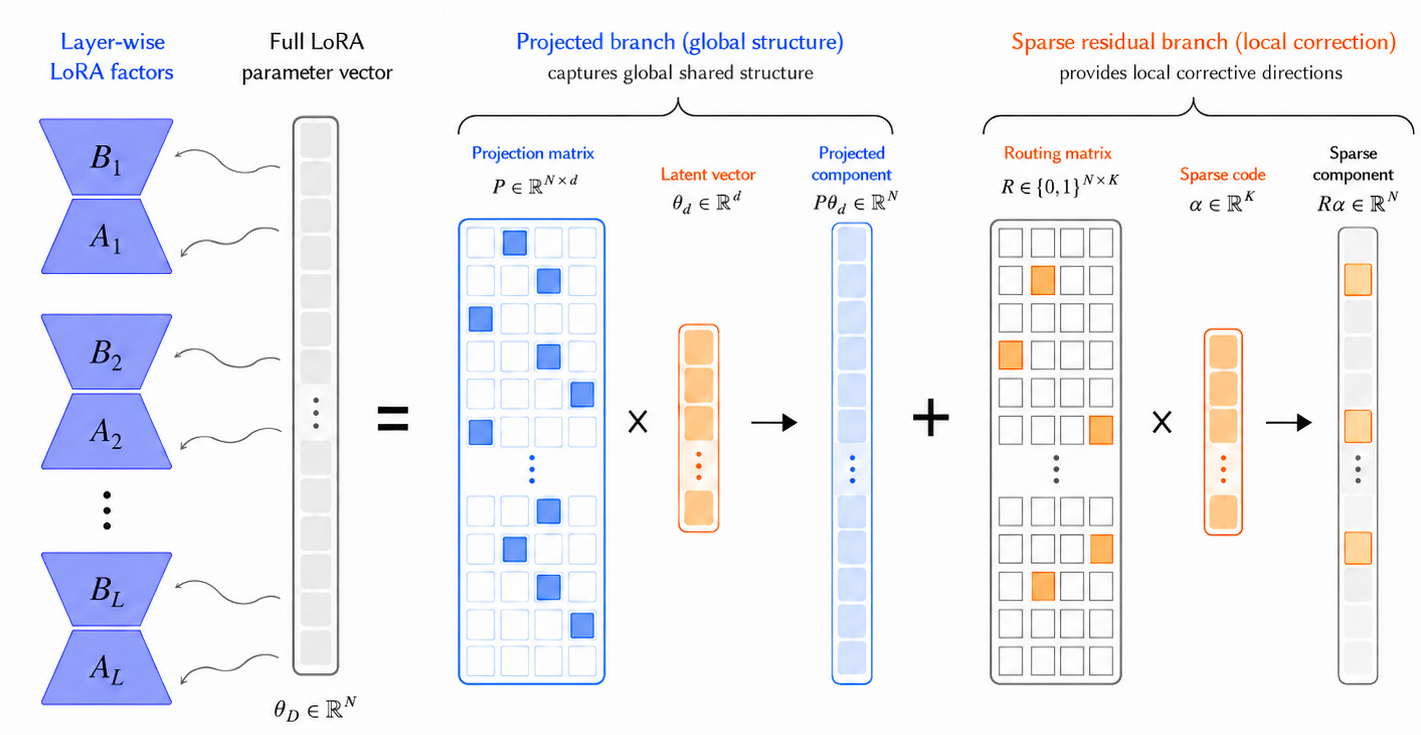
\includegraphics[width=0.65\textwidth]{framework.png}
\caption{
Overview of \textbf{ProLoSA}.
The full LoRA parameter vector is reconstructed as
$\theta_D=P\theta_d+R\alpha$, where the projected branch captures globally shared adaptation structure and the sparse residual branch restores local corrective directions on selected coordinates.
}
\label{fig:framework}
\end{figure*}

We instantiate $P$ with the normalized one-hot projection of Uni-LoRA~\citep{li2025unilora}: an assignment
$\phi:\{1,\ldots,D\}\rightarrow\{1,\ldots,d\}$, sampled once at initialization and kept fixed, maps each full-space coordinate to a latent coordinate, and
\begin{equation}
P_{ij}
=
\begin{cases}
c_j^{-1/2}, & \text{if } j=\phi(i),\\
0, & \text{otherwise},
\end{cases}
\qquad
c_j=|\{i:\phi(i)=j\}|,
\label{eq:projection_matrix_construction}
\end{equation}
so that each row of $P$ has exactly one nonzero entry and $P^\top P=I_d$.
The projected branch thus ties the $D$ LoRA coordinates into $d$ shared groups, while $R\alpha$ provides direct coordinate-wise correction on selected high-sensitivity directions.
After reconstruction, $\theta_D$ is unpacked into layer-wise factors $(A_\ell,B_\ell)$ with $\Delta W_\ell=B_\ell A_\ell$; since the final update consists of standard LoRA factors, it can be merged into the frozen backbone with no additional inference latency.

\subsection{Warmup Support Selection and Training}
\label{sec:routed_sparse_adapter}

Rather than learning a dense residual with $D$ additional parameters, {ProLoSA} activates only $K$ coordinates selected through a compressed warmup procedure, and is trained in two stages.

\emph{Stage 1: compressed warmup and support selection.}
The sparse branch is initially inactive, so $\theta_D^{(t)}=P\theta_d^{(t)}$.
Let $T$ be the total number of training steps and $\rho_{\mathrm{w}}$ the warmup ratio.
Only $\theta_d$ is optimized during the first $T_{\mathrm{pre}}=\lfloor\rho_{\mathrm{w}}T\rfloor$ steps; the model then continues to optimize $\theta_d$ for a fixed window of $T_{\mathrm{s}}=128$ steps while accumulating a SNIP-style sensitivity score~\citep{lee2018snip,he2022sparseadapter} for each full-space coordinate,
\begin{equation}
s_i
=
\sum_{t=T_{\mathrm{pre}}+1}^{T_{\mathrm{pre}}+T_{\mathrm{s}}}
\left|
\theta_{D,i}^{(t)}
g_i^{(t)}
\right|,
\qquad
g^{(t)}=\nabla_{\theta_D^{(t)}}\mathcal{L}^{(t)},
\label{eq:warmup_snip_score}
\end{equation}
which measures the accumulated first-order effect of perturbing coordinate $i$ (see Appendix~\ref{app:warmup_snip} for the derivation).
Note that the sparse branch is activated only after $T_{\mathrm{pre}}+T_{\mathrm{s}}$ steps in total: the warmup ratio $\rho_{\mathrm{w}}$ parameterizes only the score-free phase, so the compressed-only stage lasts $\lfloor\rho_{\mathrm{w}}T\rfloor+128$ steps, slightly longer than $\rho_{\mathrm{w}}T$.
The score $s_i$ is a practical \emph{proxy} for the quantity the theory asks for---the curvature-weighted off-subspace residual energy of coordinate $i$ (Appendices~\ref{sec:sparse_bias} and Appendix~\ref{app:isotropic_bias_reduction})---rather than that quantity itself: since $\theta_D=P\theta_d$ during warmup, coordinates tied to the same latent entry share the same value and are distinguished by their gradients, which reflect functional sensitivity.
Whether this proxy actually concentrates on high-energy off-subspace directions is an empirical question that experiment E5 (Appendix~\ref{sec:real_model_validation}) tests directly by measuring the captured-energy enrichment of the selected support.

\emph{Stage 2: joint training on a fixed support.}
{ProLoSA} selects the top-$K$ coordinates $\mathcal{I}=\operatorname{TopK}(\{s_i\}_{i=1}^{D},K)$, constructs $R=[e_{i_1},\ldots,e_{i_K}]$, and initializes $\alpha=0$ so that activating the residual branch does not abruptly change $\theta_D$.
Thereafter, $\theta_d$ and $\alpha$ are jointly optimized under Eq.~\eqref{eq:prolosa_main} by minimizing the downstream training loss with the backbone $W_0$ frozen, while $P$ and $R$ remain fixed.
The fixed support avoids the instability of a changing parameterization while allocating extra capacity to coordinates identified as highly sensitive after initial compressed adaptation; after training, the update is merged into the backbone as in standard LoRA.
The full procedure is summarized in Appendix~\ref{app:algorithm} (Algorithm~\ref{alg:prolosa}).

\subsection{Connection to Warmup SNIP Support Selection}
\label{app:warmup_snip}

The analysis above holds for any fixed sparse support $I$.
In practice, ProLoSA selects this support using sensitivity scores accumulated during the final fixed window of a compressed warmup stage.
Specifically, the compressed branch is first optimized for
$T_{\mathrm{pre}}=\lfloor\rho_{\mathrm{w}}T\rfloor$
steps without accumulating support-selection scores.
It is then further optimized for a fixed sensitivity-score accumulation window of
$T_{\mathrm{s}}=128$ steps, so the sparse branch is activated after $T_{\mathrm{pre}}+T_{\mathrm{s}}$ steps in total.
Throughout the warmup stage, the sparse branch is inactive and the reconstructed LoRA parameter vector is
\begin{equation}
\theta_D^{(t)}=P\theta_d^{(t)} .
\label{eq:app_warmup_reconstruction}
\end{equation}

Consider perturbing coordinate $i$ of $\theta_D^{(t)}$.
A first-order Taylor approximation of the mini-batch loss gives
\begin{equation}
\begin{aligned}
\mathcal{L}^{(t)}(\theta_D^{(t)}+\delta_i e_i)
-
\mathcal{L}^{(t)}(\theta_D^{(t)})
&\approx
g_i^{(t)}\delta_i, \\
g^{(t)}
&=
\nabla_{\theta_D^{(t)}}\mathcal{L}^{(t)} .
\end{aligned}
\label{eq:app_first_order_perturbation}
\end{equation}

Following SNIP-style saliency criteria, we measure the sensitivity of coordinate $i$ by the first-order effect of removing or perturbing its current value.
Setting $\delta_i=-\theta_{D,i}^{(t)}$ gives
\begin{equation}
\left|
\theta_{D,i}^{(t)}g_i^{(t)}
\right|.
\label{eq:app_single_step_snip_score}
\end{equation}

Accumulating this quantity over the fixed sensitivity-score accumulation window yields
\begin{equation}
s_i
=
\sum_{t=T_{\mathrm{pre}}+1}^{T_{\mathrm{pre}}+T_{\mathrm{s}}}
\left|
\theta_{D,i}^{(t)}g_i^{(t)}
\right|,
\qquad
T_{\mathrm{s}}=128.
\label{eq:app_warmup_snip_score}
\end{equation}

Coordinates with large $s_i$ are those whose perturbation has a consistently large first-order effect on the training loss during this compressed adaptation window.
Selecting the top-$K$ coordinates therefore provides a data-dependent heuristic for identifying directions where the compressed branch may require local correction.
This support-selection rule does not guarantee the globally optimal support in the theoretical sense, but it aligns the sparse residual budget with coordinates that are locally influential during the final fixed window of the compressed warmup trajectory.


\subsection{Training Algorithm}
\label{app:algorithm}

Algorithm~\ref{alg:prolosa} summarizes the full training procedure of {ProLoSA}.
The first stage performs compressed-only training for $T_{\mathrm{pre}}+T_{\mathrm{s}}$ steps, with coordinate-wise sensitivity scores accumulated only during the final fixed $T_{\mathrm{s}}=128$-step window; the warmup ratio $\rho_{\mathrm{w}}$ determines only $T_{\mathrm{pre}}=\lfloor\rho_{\mathrm{w}}T\rfloor$, so the sparse branch is activated at step $\lfloor\rho_{\mathrm{w}}T\rfloor+128$ rather than at exactly $\rho_{\mathrm{w}}T$.
The second stage fixes the selected sparse support and jointly optimizes the projected and sparse residual branches.

\begin{algorithm}[!htbp]
\small
\caption{{ProLoSA} with Warmup SNIP Support Selection}
\label{alg:prolosa}
\begin{algorithmic}[1]
\REQUIRE Frozen backbone $W_0$; projection matrix $P$; sparse budget $K$; warmup ratio $\rho_{\mathrm{w}}$; sensitivity-score accumulation steps $T_{\mathrm{s}}=128$; total training steps $T$.
\STATE Initialize compressed latent parameter $\theta_d$.
\STATE Set sparse adapter inactive and initialize score vector $s \leftarrow 0_D$.
\STATE Set $T_{\mathrm{pre}}\leftarrow\lfloor\rho_{\mathrm{w}}T\rfloor$.
\FOR{$t=1$ to $T_{\mathrm{pre}}$}
    \STATE Reconstruct $\theta_D^{(t)} \leftarrow P\theta_d^{(t)}$ and unpack it into $\{A_\ell,B_\ell\}_{\ell\in\mathcal{L}}$.
    \STATE Compute mini-batch loss $\mathcal{L}^{(t)}$.
    \STATE Update $\theta_d$ by back-propagation.
\ENDFOR
\FOR{$t=T_{\mathrm{pre}}+1$ to $T_{\mathrm{pre}}+T_{\mathrm{s}}$}
    \STATE Reconstruct $\theta_D^{(t)} \leftarrow P\theta_d^{(t)}$ and unpack it into $\{A_\ell,B_\ell\}_{\ell\in\mathcal{L}}$.
    \STATE Compute mini-batch loss $\mathcal{L}^{(t)}$ and gradient $g^{(t)} \leftarrow \nabla_{\theta_D^{(t)}}\mathcal{L}^{(t)}$.
    \STATE Accumulate scores $s \leftarrow s+\left|\theta_D^{(t)}\odot g^{(t)}\right|$.
    \STATE Update $\theta_d$ by back-propagation.
\ENDFOR
\STATE Select sparse support $\mathcal{I}\leftarrow\operatorname{TopK}(s,K)$.
\STATE Construct $R=[e_{i_1},\ldots,e_{i_K}]$ for $\mathcal{I}=\{i_1,\ldots,i_K\}$ and initialize $\alpha\leftarrow 0$.
\FOR{$t=T_{\mathrm{pre}}+T_{\mathrm{s}}+1$ to $T$}
    \STATE Reconstruct $\theta_D \leftarrow P\theta_d+R\alpha$ and unpack it into $\{A_\ell,B_\ell\}_{\ell\in\mathcal{L}}$.
    \STATE Compute mini-batch loss $\mathcal{L}^{(t)}$.
    \STATE Update $\theta_d$ and $\alpha$ by back-propagation.
\ENDFOR
\RETURN Trained $\theta_d$, $\alpha$, and fixed routing matrix $R$.
\end{algorithmic}
\end{algorithm}



\clearpage
\section{Mechanism Experiments}
\label{app:mechanism}
\subsection{Projection-Blind Synthetic Validation of the Bias--Variance Trade-off}
\label{sec:synthetic}

We isolate the statistical effect of compression in a controlled Gaussian sequence estimation problem that is \emph{projection-blind}: the target is generated independently of the projection matrix, so that no favorable alignment or artificial mismatch is built into the ground truth.
The target's energy \emph{profile}, in contrast, is deliberately controlled---heavy-tailed here and dense Gaussian in Appendix~\ref{sec:synthetic_failure}---to instantiate the recoverable and diffuse off-subspace regimes that the theory distinguishes.
The mixture is used only to generate a problem instance.
Specifically, independently for each coordinate, we draw
$b_j\sim\operatorname{Bernoulli}(\pi)$,
$g_j\sim\mathcal N(0,1)$, and $T_j\sim t_\nu$, and set
\begin{equation}
\Theta_j^\star
=
(1-b_j)\tau_0g_j
+
b_j\tau_1\sqrt{\frac{\nu-2}{\nu}}\,T_j .
\label{eq:synthetic_gt}
\end{equation}
The factor $\sqrt{(\nu-2)/\nu}$ standardizes $T_j$ to unit variance, so $\tau_1$ is the standard deviation---not the scale parameter---of the heavy-tailed component.
We use $\pi=0.01$, $\tau_0=0.005$, $\tau_1=0.5$, and $\nu=3$.
This zero-mean i.i.d.\ problem-generation law is isotropic with
\begin{equation}
v
=
\mathbb E_{\mathcal Q}[(\Theta_j^\star)^2]
=
(1-\pi)\tau_0^2+\pi\tau_1^2
=
2.52475\times10^{-3}.
\label{eq:synthetic_target_energy}
\end{equation}
Using seed 13, we draw one realization $\theta^\star$ of $\Theta^\star$ and an independent $P$ and hold both fixed across all noise levels and all $M=200$ trials.
Only the observation noise is resampled:
$y^{(m)}=\theta^\star+(\sigma_y/\sqrt{n_{\mathrm{eff}}})\epsilon^{(m)}$ with
$\epsilon^{(m)}\sim\mathcal N(0,I_D)$.
Thus, in every trial, the same realized vector $\theta^\star$ remains the population optimum; the mixture describes variation across possible synthetic problem instances, whereas Proposition~\ref{prop:energy_noise} additionally averages over that generation law.
Each method solves the constrained least-squares problem
\(\hat{\theta}_{\mathcal S}=\arg\min_{\theta\in\mathcal S}\frac{1}{2}\|y-\theta\|_2^2\),
with \(\mathcal S=\mathbb{R}^D\) for LoRA, \(\mathcal S=\mathrm{col}(P)\) for Uni-LoRA, and the sparse-augmented space \(\mathrm{col}([P,E_{\mathcal I}])\) for ProLoSA, whose support \(\mathcal I\) is the top-\(K\) coordinates of the post-warmup residual \(|y-PP^\top y|\)---the estimation-setting analog of the warmup SNIP score in Eq.~\eqref{eq:warmup_snip_score}---and we measure the population excess risk \(\frac{1}{2}\|\hat{\theta}-\theta^\star\|_2^2\).
We use \(D=4096\), \(d=16\), \(K=32\), and \(n_{\mathrm{eff}}=512\) (full configuration in Appendix~\ref{app:exp_details}); the realized mixture draw has \(33\) heavy-tailed coordinates, and the largest \(32\) residual coordinates carry \(98.8\%\) of the off-subspace energy.

Figure~\ref{fig:synthetic_validation} reveals the predicted transition between variance- and bias-dominated regimes. 
The risk of full-space LoRA grows rapidly with \(\sigma_y\) because its unconstrained estimator retains noise in all \(D\) coordinates, whereas Uni-LoRA suppresses estimation variance but pays a projection-bias floor since the independently generated \(\theta^\star\) need not lie in \(\mathrm{col}(P)\). 
Uni-LoRA is therefore worse than LoRA at small noise but preferable once the full-space variance grows large---exactly the crossover of Eq.~\eqref{eq:compression_condition}.
For the fixed realized target and projection,
$\hat v_\perp=\|(I-PP^\top)\theta^\star\|_2^2/(D-d)=2.6486\times10^{-3}$.
Equation~\eqref{eq:conditional_compressed_risk} therefore predicts the exact conditional crossover
$\sigma_y^\ast=\sqrt{n_{\mathrm{eff}}\hat v_\perp}=1.165$, matching the observed intersection in Figure~\ref{fig:synthetic_validation}A.
The overall realized energy $\|\theta^\star\|_2^2/D=2.6444\times10^{-3}$ is nearly identical because $P$ is independent and $D$ is large, but it is $\hat v_\perp$, rather than the ensemble quantity $v$, that gives the fixed-instance threshold.

Panels B--C make the mechanism explicit via the empirical decomposition
\(\mathrm{Bias}=\frac{1}{2}\|\bar{\theta}-\theta^\star\|_2^2\)
and
\(\mathrm{Variance}=\frac{1}{2M}\sum_{m}\|\hat{\theta}^{(m)}-\bar{\theta}\|_2^2\)
across the \(M\) noise realizations, where \(\bar{\theta}\) is the mean estimate.
Both components use the same fixed $(\theta^\star,P)$ and the same $M$ estimates. With denominator $M$ in the empirical variance, their sum equals the empirical mean excess risk exactly; the plug-in bias includes finite-$M$ estimation noise.

\paragraph{Conditioning and aggregation.}
A repeated training/noise trial does not draw a new optimum. If a separate experiment changes the target to $\theta_t^\star$, we first compute its own conditional mean $\mu_t=\mathbb E[\hat\theta\mid t]$, bias $B_t=\tfrac12\|\mu_t-\theta_t^\star\|^2$, and variance $V_t=\tfrac12\mathbb E[\|\hat\theta-\mu_t\|^2\mid t]$. A declared task average may report $\mathbb E_t[B_t+V_t]$, but estimates from distinct targets must not be pooled into a single fixed-target decomposition. In particular, pooled estimator dispersion includes variation of $\mu_t$ across tasks; adding it to an independently averaged conditional bias double-counts or misattributes variability. Concentrated and diffuse targets, different target strengths, and different source distributions are therefore separate experiments. Random supports, when used, contribute to estimator variability conditional on the fixed target. The matched-budget and dense-failure curves below follow this convention throughout the noise sweep.

\paragraph{Conditional sequence results.}
At \(\sigma_y=0.5\), LoRA has essentially no bias but incurs an excess risk of \(1.00\) almost entirely from variance; Uni-LoRA reduces this variance to nearly zero but its projection bias raises the total risk to \(5.41\); ProLoSA corrects the mismatch and reaches \(0.08\). 
At \(\sigma_y=1.5\), the variance of LoRA drives its risk to \(9.00\), Uni-LoRA remains at its bias floor of \(5.44\), and ProLoSA attains a risk of only \(0.47\).
Sparse correction thus recovers most of the approximation error without giving up the variance-reduction benefit of compression---precisely because the off-subspace energy of the heavy-tailed target is concentrated on a few large coordinates, the recoverable case identified in Appendix~\ref{sec:when_fails}.

\paragraph{Matched-budget comparison.}
The comparison above spends $d+K=48$ parameters for ProLoSA against $d=16$ for Uni-LoRA, so it demonstrates bias reduction but not yet the matched-budget claim of Proposition~\ref{prop:matched_budget}.
Figure~\ref{fig:synthetic_matched_budget} therefore fixes the total budget at $B=d+K=48$ and compares, on the identical fixed target and noise realizations, a compressed-only estimator of dimension $B$ against hybrids ($d=16$, $K=32$) whose supports are random, noise-dependent (top-$K$ residual, the SNIP analog), or oracle (top-$K$ of the true off-subspace residual).
Here ``oracle'' means that the support may inspect the fixed target $\theta^\star$; the top-$K$ rule is a target-informed surrogate, not an exhaustive search over all size-$K$ supports.
The results are consistent with both parts of the proposition.
First, the random hybrid nearly ties the $B$-dimensional compressed-only estimator across the entire noise range (e.g., $5.37$ vs.\ $5.36$ at $\sigma_y=0.5$ and $5.46$ vs.\ $5.45$ at $\sigma_y=1.5$); the fixed $B$-dimensional projection has a conditional bias floor of $5.349$, close to both curves.
This is the high-dimensional single-instance counterpart of Corollary~\ref{cor:random_support}, whose equality is an ensemble expectation under the isotropic target law.
Second, informed supports win by orders of magnitude on this concentrated target ($0.08$ at $\sigma_y=0.5$), because the target-informed top-$K$ directions recover more energy than the realized bias difference between the $d$- and $B$-dimensional projections (Eq.~\eqref{eq:fixed_matched_budget_condition}): their coordinates contain $98.8\%$ of the residual's coordinatewise energy, and projection onto the resulting augmented subspace removes $99.0\%$ of the projection bias.
The same panel also quantifies the selection-variance effect of the remark after Proposition~\ref{prop:matched_budget}: the noise-dependent support tracks the oracle at small $\sigma_y$ but degrades relative to it as noise grows ($0.47$ vs.\ $0.16$ at $\sigma_y=1.5$), while still improving over compressed-only by an order of magnitude.
Finally, comparing the full-space estimator with the $B=48$ compressed-only estimator answers the budget-level question of when compression itself pays.
Denoting that fixed $B$-dimensional projection by $P_B$,
$\hat v_{\perp,B}=\|(I-P_BP_B^\top)\theta^\star\|_2^2/(D-B)=2.6427\times10^{-3}$, so Eq.~\eqref{eq:conditional_compressed_risk} predicts
$\sigma_y^\ast=\sqrt{n_{\mathrm{eff}}\hat v_{\perp,B}}=1.163$, matching the observed crossing near $1.16$.

\begin{figure*}[t]
    \centering
    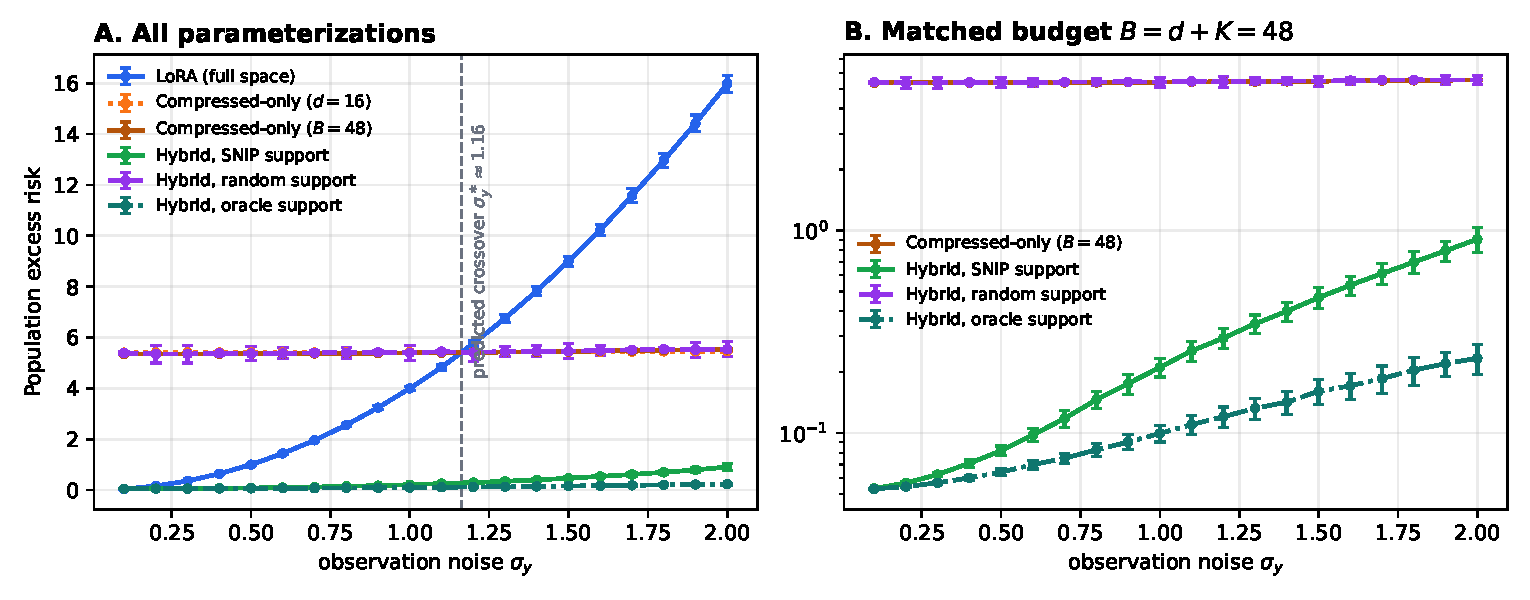
\includegraphics[width=0.9\textwidth]{synthetic_matched_budget.pdf}
    \caption{
    \textbf{Matched-budget comparison in the projection-blind sequence model} ($B=d+K=48$, heavy-tailed target).
    \textbf{A:} population excess risk of all parameterizations; the dashed vertical line marks the fixed-instance full-space/compressed crossover $\sigma_y^\ast\approx 1.16$ predicted by Eq.~\eqref{eq:conditional_compressed_risk}.
    \textbf{B:} matched-budget methods only (log scale). The random-support hybrid nearly coincides with the $B$-dimensional compressed-only estimator on this instance, consistent with the ensemble equality in Corollary~\ref{cor:random_support}; informed supports recover most of the bias, and the gap between the noise-dependent (SNIP-analog) and target-informed top-$K$ supports grows with $\sigma_y$, visualizing the selection-variance effect.
    }
    \label{fig:synthetic_matched_budget}
\end{figure*}

\begin{figure*}[t]
    \centering
    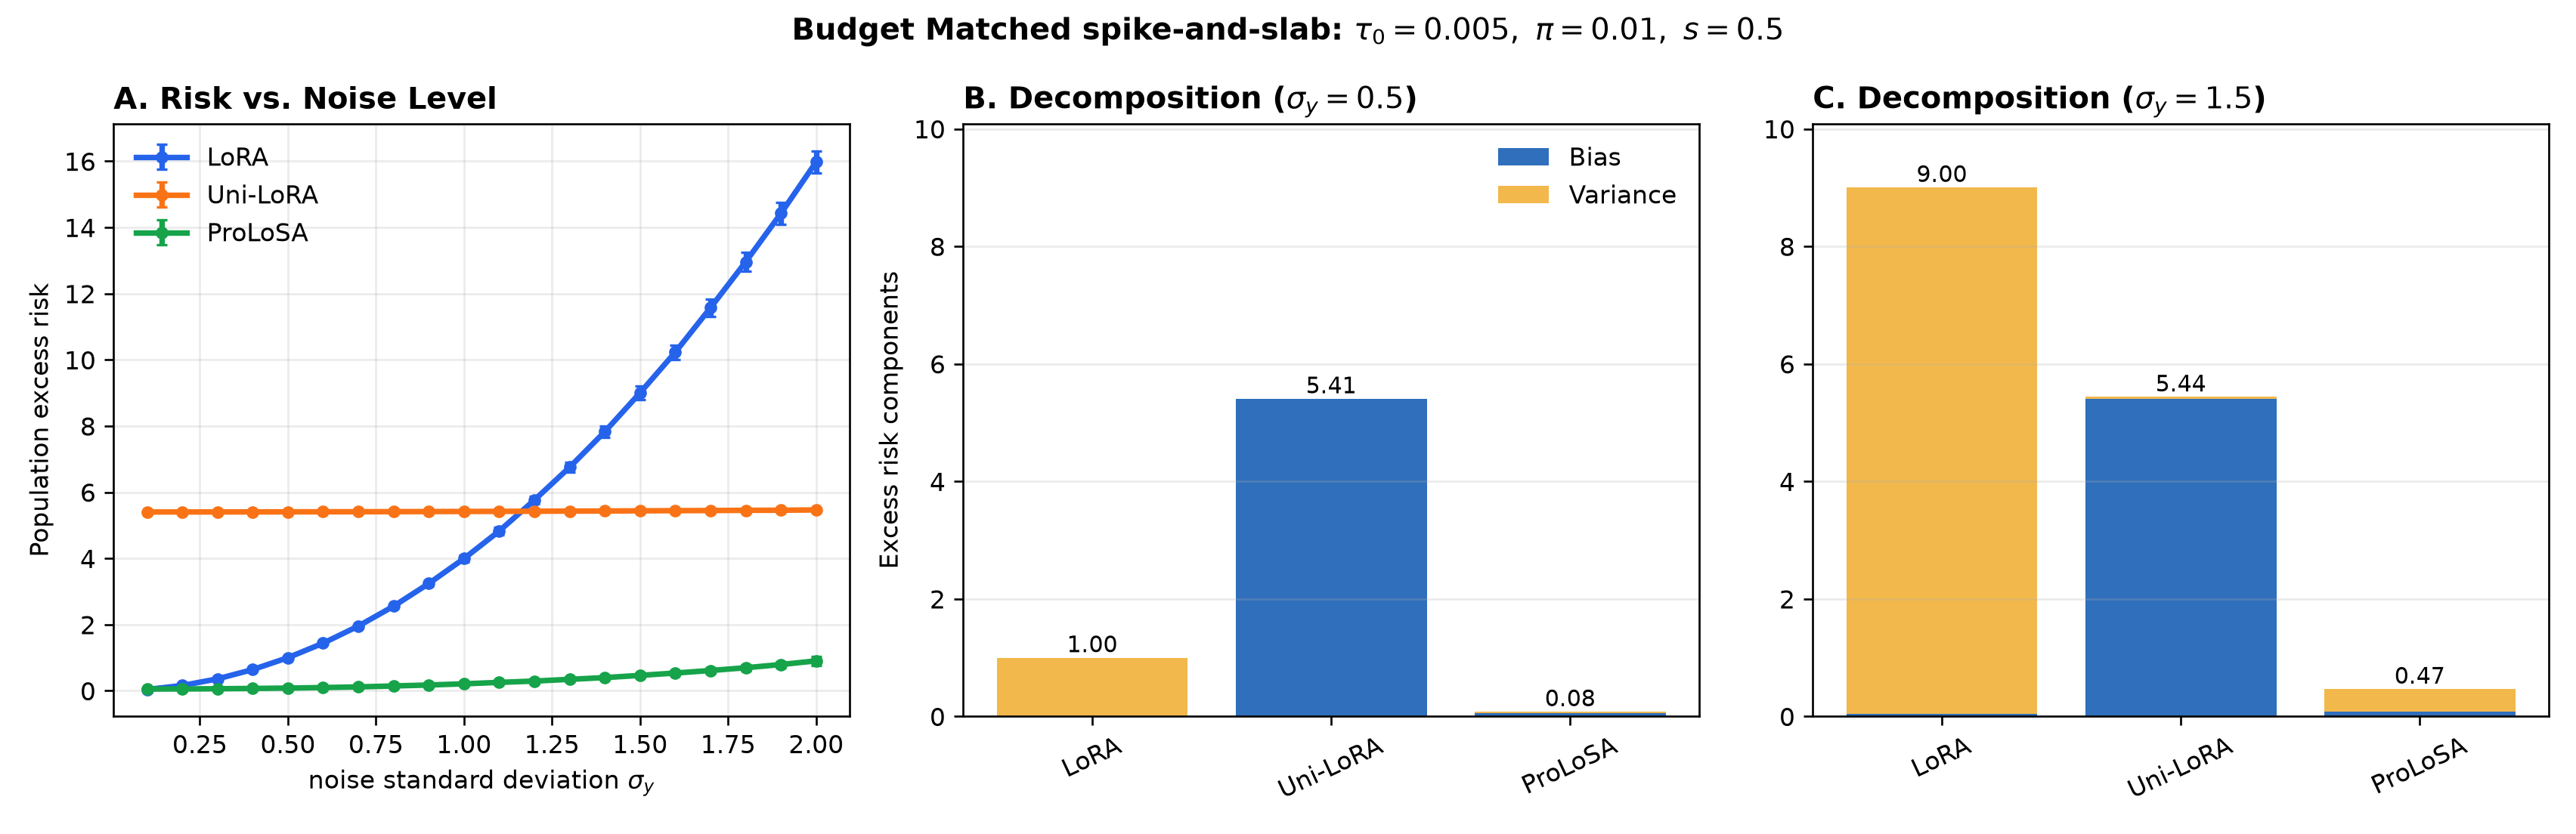
\includegraphics[width=0.65\textwidth]{synthetic_blind_validation.png}
    \caption{
    \textbf{Projection-blind synthetic validation of the compression bias--variance trade-off.}
    One ground-truth update is sampled independently of the projection matrix; both remain fixed across all trials and noise levels. The observation-noise level \(\sigma_y\) controls estimation variance.
    \textbf{A:} population excess risk as \(\sigma_y\) increases; the LoRA/Uni-LoRA crossover at \(\sigma_y\approx 1.16\) matches the conditional form of Proposition~1 in Eq.~\eqref{eq:conditional_compressed_risk}, while ProLoSA retains the variance reduction of compression and corrects most of its bias.
    \textbf{B and C:} empirical bias--variance decompositions at \(\sigma_y=0.5\) and \(\sigma_y=1.5\), respectively.
    }
    \label{fig:synthetic_validation}
\end{figure*}

\subsection{The Bias-Dominated Regime: When Compression Uniformly Fails}
\label{sec:synthetic_failure}

The heavy-tailed mixture above is favorable to sparse correction because its off-subspace residual is concentrated; its modest average energy also lets compression become beneficial once observation noise is sufficiently large.
Proposition~1 predicts that the latter picture reverses when the target becomes dense and high-energy.
To test this failure prediction, we replace the problem-generation law in Eq.~\eqref{eq:synthetic_gt} with
$\Theta_j^\star\sim\mathcal N(0,\tau^2)$, $\tau=0.125$, again draw a single target independently of $P$, and hold it fixed across all observation-noise trials.
The ensemble energy is $v=\tau^2=1.56\times10^{-2}$; for the realized pair $(\theta^\star,P)$, the exact conditional value is
$\hat v_\perp=1.5685\times10^{-2}$.
Both exceed the effective noise $\sigma_y^2/n_{\mathrm{eff}}$ over the entire tested range (at most $7.8\times10^{-3}$ at $\sigma_y=2$), while all remaining settings are unchanged.
This construction models adaptation regimes requiring large, dense parameter changes.

Figure~\ref{fig:synthetic_failure} confirms both parts of the prediction.
First, the risk of Uni-LoRA stays pinned at its fixed-instance projection-bias floor
$\tfrac{1}{2}(D-d)\hat v_\perp=32.0$, which exceeds the risk of full-space LoRA at every tested noise level (LoRA reaches only $16.0$ at $\sigma_y=2$).
Compression is therefore \emph{uniformly} harmful in the tested range, and the conditional crossover
$\sigma_y^\ast=\sqrt{n_{\mathrm{eff}}\hat v_\perp}=2.83$ lies outside it.
Second, ProLoSA no longer helps: with the off-subspace energy spread diffusely over all $D-d$ residual directions, the top-$K$ support carries only $6.9\%$ of the target energy, so the sparse correction recovers only a negligible fraction of the bias and its risk curve nearly coincides with that of Uni-LoRA ($30.4$ vs.\ $32.0$ at $\sigma_y=1.5$)---exactly the unrecoverable case identified in Appendix~\ref{sec:when_fails}.
These results suggest, within a single framework, why compressed LoRA thrives in downstream fine-tuning, whose updates are typically low-energy and approximately sparse (the variance-dominated, recoverable regime), yet is a poor fit for tasks requiring large, dense updates, where any fixed low-dimensional parameterization---with or without sparse correction---is limited.

\begin{figure*}[t]
    \centering
    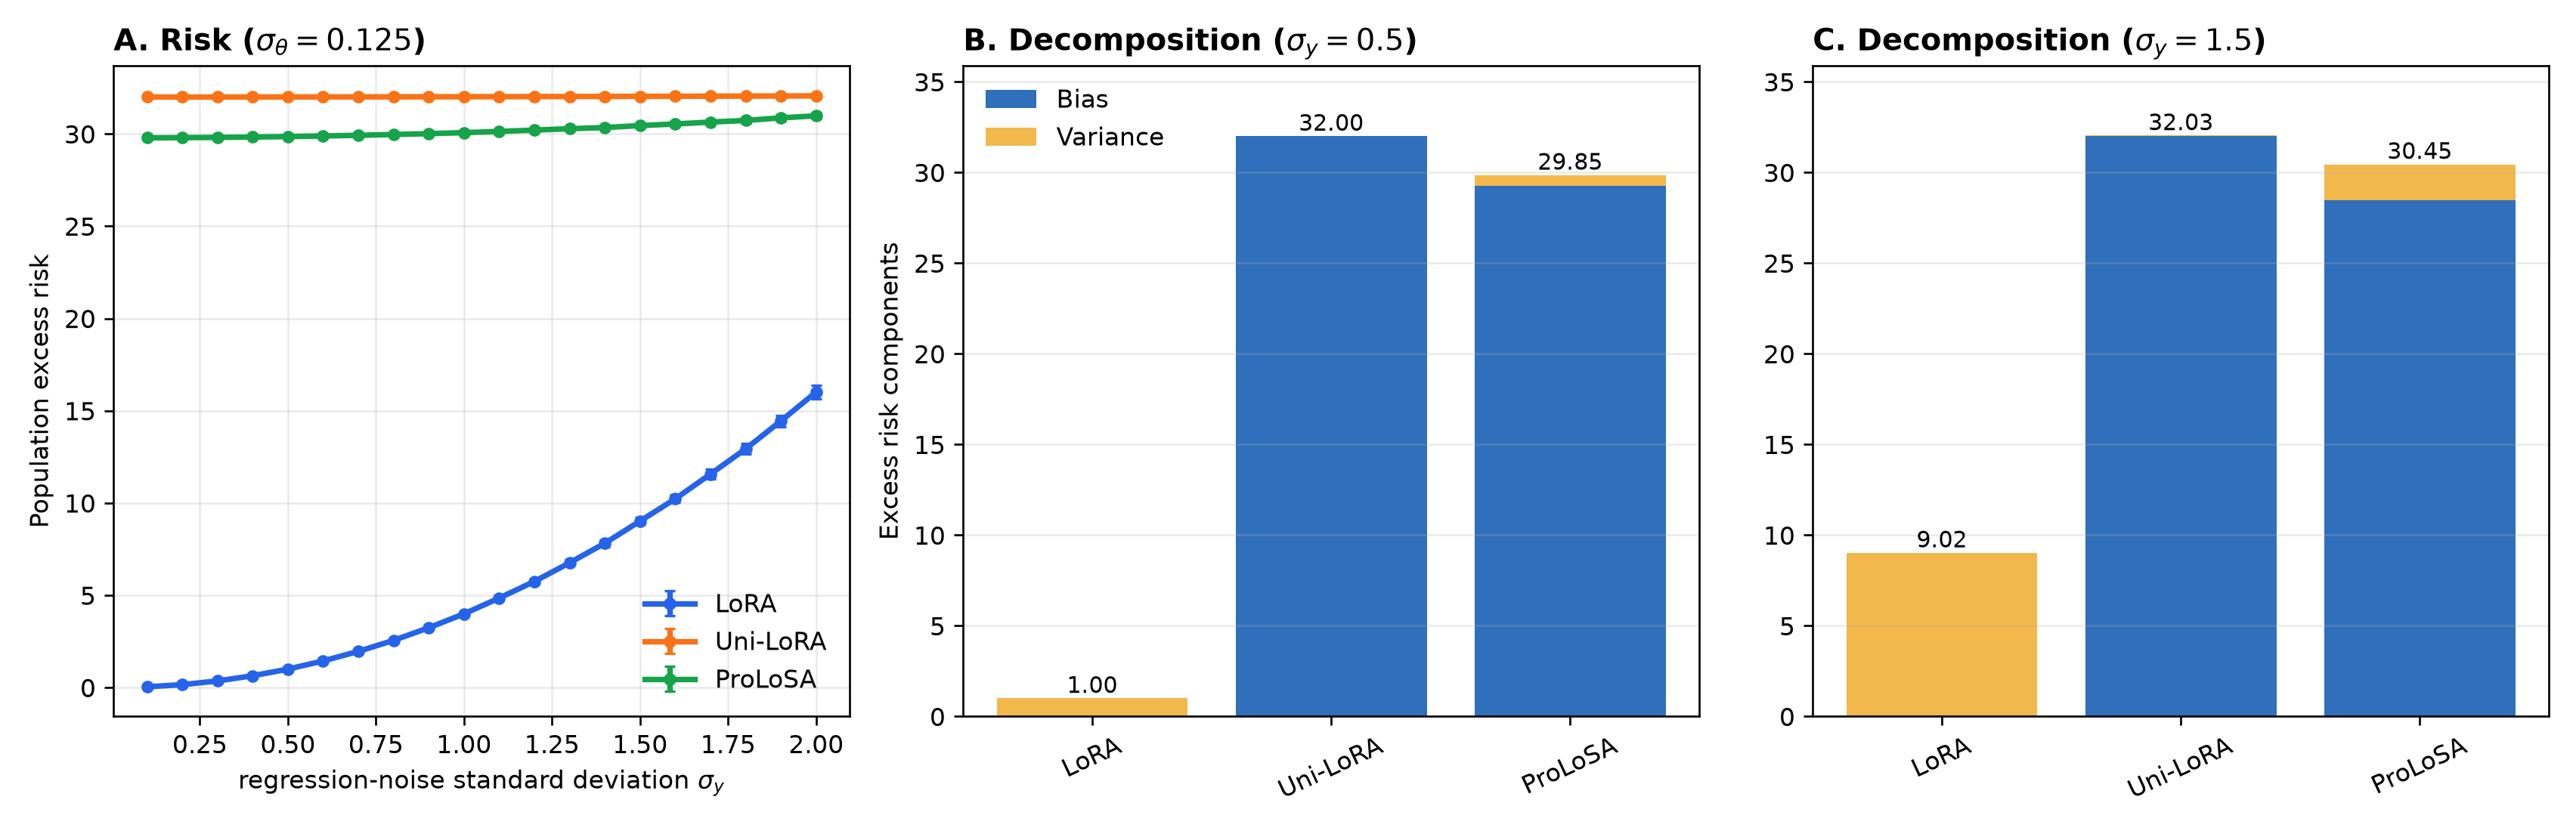
\includegraphics[width=0.65\textwidth]{synthetic_bias_dominated.png}
    \caption{
    \textbf{The bias-dominated failure regime.}
    With a fixed dense Gaussian target ($\tau=0.125$, with realized $\hat v_\perp>\sigma_{\mathrm{eff}}^2$ throughout the tested range), Uni-LoRA is pinned at its bias floor of $32.0$, uniformly worse than LoRA (\textbf{A}), and ProLoSA recovers only a negligible fraction of the diffuse bias (\textbf{B}, \textbf{C}), as predicted by Proposition~1.
    }
    \label{fig:synthetic_failure}
\end{figure*}


\subsection{From the Sequence Model to a Transformer Block}
\label{sec:transformer_synthetic}

The sequence model of Appendices~\ref{sec:synthetic} and~\ref{sec:synthetic_failure} tests the fixed-instance identity in Eq.~\eqref{eq:conditional_compressed_risk}, but deliberately removes several properties of neural
network fine-tuning, including nonlinear parameterization, anisotropic
curvature, finite-step optimization, and data-dependent support selection.
We therefore run a second controlled teacher--student experiment on a single
Transformer block, in which the ground-truth update remains known and its
energy profile controllable. The goal is not the numerical threshold of
Eq.~\eqref{eq:energy_noise_condition}, which is specific to the isotropic
sequence model, but whether the qualitative bias--variance predictions
survive once these idealizations are removed.

\paragraph{Setup.}
We use a standard Transformer block ($d_{\mathrm{model}}=64$, sequence length
$T=32$, $d_{\mathrm{ff}}=256$; multi-head self-attention, a two-layer MLP,
LayerNorm, and residual connections), whose base parameters $W_0$ are
pretrained on a generic synthetic sequence-regression task and then frozen.
We adapt the query and value projections and work directly in the vectorized
\emph{weight-update} space
\begin{equation}
    \theta
    =
    \operatorname{vec}(\Delta W_q,\Delta W_v)
    \in\mathbb{R}^{D},
    \qquad
    D=8192,
\end{equation}
in which the compression $P\theta_d$, the sparse routing, and all energy
measurements are defined; unlike the LoRA factor space, this space is
identifiable (cf.\ the remark after Proposition~\ref{prop:energy_noise}).
The teacher plants a target $\theta^\star$ with one of two energy profiles:
\emph{concentrated} (the sparse heavy-tailed mixture of
Eq.~\eqref{eq:synthetic_gt}) or \emph{diffuse} (dense Gaussian).
Each planted update is then rescaled by a common scalar so that its
functional displacement
\begin{equation}
    \delta_{\mathrm{func}}
    =
    \mathbb{E}_{x}\big[\|f(x;W_0+\Delta W^\star)-f(x;W_0)\|_2^2\big]
    \big/
    \mathbb{E}_{x}\big[\|f(x;W_0)\|_2^2\big]
    \label{eq:functional_displacement}
\end{equation}
equals $10\%$ (concentrated) or $100\%$ (diffuse) of the output variance;
the two profiles thus differ in both magnitude and concentration, mirroring
the ``modest fine-tuning update vs.\ large distribution shift'' contrast of
Appendices~\ref{sec:synthetic}--\ref{sec:synthetic_failure}.
Both targets are almost entirely off-subspace (off-subspace fraction
$\approx 0.99$), but the top-$K$ ($K=64$) coordinates of the residual carry
$99\%$ of its energy in the concentrated profile versus $7\%$ in the diffuse
profile---recoverable versus unrecoverable by construction.
Training data are $y_i=f(x_i;W_0+\Delta W^\star)+\varepsilon_i$ with
$\varepsilon_i\sim\mathcal{N}(0,\sigma_y^2I)$, where $f$ returns the
$d_{\mathrm{model}}$-dimensional pooled hidden representation; the
vector-valued output keeps the planted directions functionally observable.

\paragraph{Compared parameterizations.}
With $W_0$ frozen, every method optimizes its own parameters with AdamW for a
fixed step budget: full fine-tuning of the adapted matrices ($8192$
parameters), rank-$4$ LoRA ($1024$), a matched-budget compressed
parameterization $\theta=P\theta_d$ with $B=d+K=128$, ProLoSA with $d=64$
projected and $K=64$ routed coordinates using the true two-stage warmup SNIP
protocol of Appendix~\ref{sec:routed_sparse_adapter}, a random-support hybrid,
and an oracle-support hybrid.
The saved Transformer implementation defines its target-informed oracle support by
\begin{equation}
 s_i^{\mathrm{oracle}}=\widehat H_{ii}(\theta_i^\star)^2,
 \label{eq:transformer_oracle}
\end{equation}
where $\widehat H$ is a diagonal empirical Gauss--Newton proxy. This is a score on the planted update, not the $H$-projected residual or the exact joint bias reduction. The support is fixed within each teacher grid. The calibration run estimates its own curvature proxy, so its oracle support need not match the noisy grid even when the planted target is unchanged.
We sweep $n\in\{64,\ldots,4096\}$ and $\sigma_y\in\{0.1,\ldots,2.0\}$ with
$M=20$ training-set/optimization seeds per cell. For each profile, the teacher update, pretrained backbone, projections, and noiseless test inputs are fixed before iterating over $n$, noise, and training seed; the full
configuration is given in Appendix~\ref{app:transformer_details}.

\paragraph{Function-space measurement.}
Since parameter-space distances are misleading under nonlinear and
overparameterized parameterizations, we measure excess risk and its
decomposition in function space on a large noiseless test set from the
teacher distribution: with $\bar f(x)=\frac{1}{M}\sum_{m=1}^{M}f_{\hat\theta^{(m)}}(x)$,
\begin{align}
 \mathrm{Bias}_{\mathrm{func}}
 &=\mathbb E_{x,c}\big[(\bar f_c(x)-f_{\theta^\star,c}(x))^2\big],\\
 \mathrm{Variance}_{\mathrm{func}}
 &=\frac1M\sum_{m=1}^M\mathbb E_{x,c}
 \big[(f_{\hat\theta^{(m)},c}(x)-\bar f_c(x))^2\big].
 \label{eq:functional_bias_variance}
\end{align}
Here $\mathbb E_{x,c}$ averages test examples and output coordinates. The stored Transformer metric is excess prediction MSE, without the factor $1/2$ used in the sequence model; its empirical mean equals these two components' sum. Each decomposition is conditional on one teacher and fixed test inputs. We do not pool the two profiles. The 20-seed noisy grid and two-seed noiseless calibration are separate cells, and neither their bias nor their variance is combined. Rechecking the 10,108 saved trials reproduces all 518 cell risk means and standard deviations; every stored function-space bias--variance sum matches its cell mean. The original Transformer Python sources and per-run predictions are not retained in this workspace: fixed-teacher control is supported by saved runner bytecode, logs, and target metadata, but the decomposition cannot be independently recomputed from raw predictions here.

\paragraph{Approximation floors.}
Noiseless large-sample fits confirm that the two constructions instantiate
the intended regimes in function space: the matched-budget compressed
parameterization has an approximation floor of $0.0047$ under the
concentrated target versus $0.041$ under the diffuse target ($\approx 9\times$
larger), and the oracle hybrid removes $99\%$ of the concentrated floor
(to $6\times 10^{-5}$) but only $13\%$ of the diffuse floor (to $0.035$)
(Appendix~\ref{app:transformer_details}).

\paragraph{Results: sample-size crossover and its noise shift.}
Figure~\ref{fig:transformer_risk} shows excess prediction MSE as a
function of $n$.
The qualitative predictions of Appendix~\ref{sec:testable_predictions} hold in
both regimes: at small $n$, full-space methods are variance-dominated and the
compressed parameterization wins by up to an order of magnitude; as $n$
grows, LoRA crosses below the compressed baseline---at
$n\approx 2^9$--$2^{10}$ for the diffuse target and
$n\approx 2^{11}$ for the concentrated target at $\sigma_y=0.5$---and the
crossover point moves to larger $n$ as the label noise increases (at
$\sigma_y=2$ it exceeds $n=10^3$ in both regimes), exactly the
$n^\star\propto A_{\mathrm{var}}/B_{\mathrm{proj}}$ shift predicted by
Eq.~\eqref{eq:risk_gap_n}.

\paragraph{Results: decomposition, recoverability, and matched budgets.}
Figure~\ref{fig:transformer_biasvar} reports the function-space
decomposition of Eq.~\eqref{eq:functional_bias_variance}.
At $n=64$ the excess risk of LoRA is almost entirely variance, which every
compressed parameterization suppresses by an order of magnitude; at $n=4096$
the compressed methods are pinned at their bias floors while LoRA's bias is
far smaller---the predicted reversal of the bias and variance orderings.
Sparse residual correction behaves exactly as the recoverability analysis
predicts: under the concentrated target, ProLoSA reduces the compressed bias
floor by roughly half (excess risk $0.0030$ vs.\ $0.0052$ at $n=4096$,
$\sigma_y=1$) with the oracle support reaching $5.6\times 10^{-4}$, whereas
under the diffuse target even the oracle support barely helps
($0.0356$ vs.\ $0.0412$), so the limitation is the energy profile itself,
not support selection.
The matched-budget prediction also carries over: the random-support hybrid
never beats the compressed baseline of the same budget, tying it under the
concentrated target ($0.0053$ vs.\ $0.0052$) and running slightly worse under
the diffuse target ($0.0439$ vs.\ $0.0412$)---a deviation from the exact
isotropic tie of Corollary~\ref{cor:random_support} that is consistent with
anisotropic curvature.
Finally, the experiment also exposes the predicted cost of data-dependent
selection: in the small-$n$, high-noise corner of the concentrated regime
(e.g., $n=64$, $\sigma_y=1.5$), ProLoSA's noisy warmup scores select
unreliable supports and it falls behind the compressed baseline
($0.105$ vs.\ $0.066$), the selection-variance effect anticipated in the
remark after Proposition~\ref{prop:matched_budget}.
In sum, all four qualitative predictions persist under nonlinear
parameterization, anisotropic curvature, finite-step optimization, and
data-dependent support selection, and the observed deviations occur precisely
where the theory's idealizations are known to break.

\begin{figure*}[t]
    \centering
    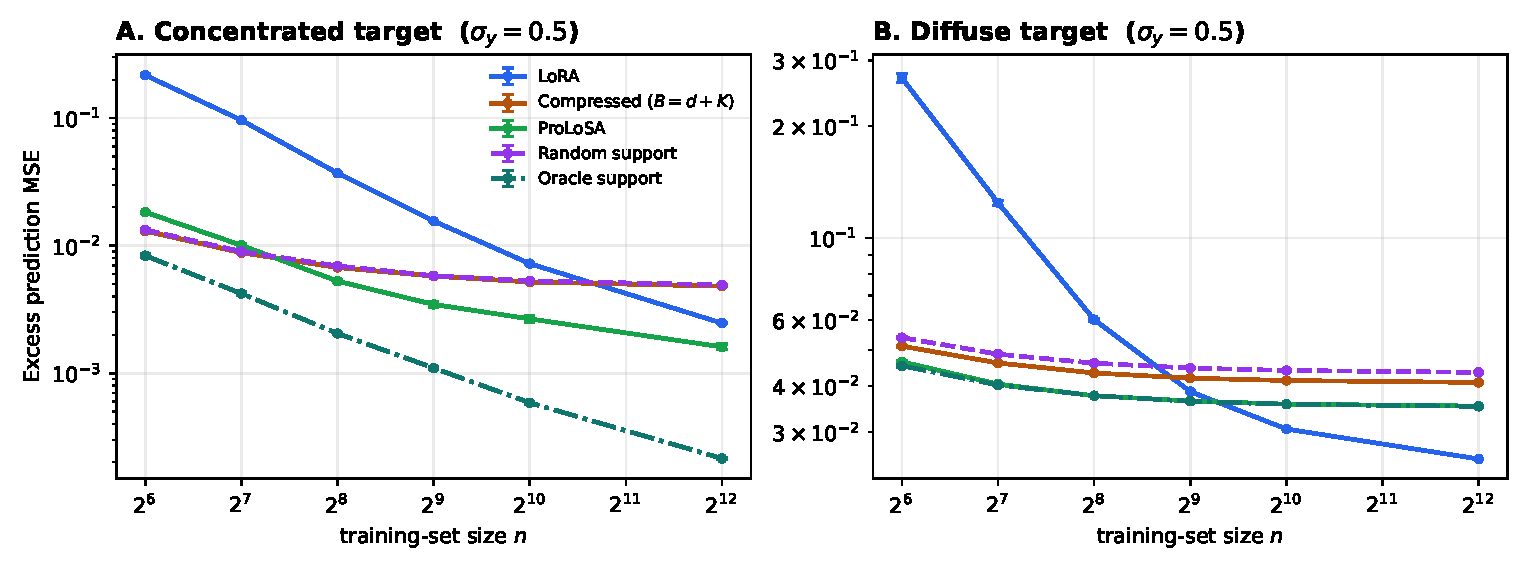
\includegraphics[width=0.95\textwidth]{transformer_risk_vs_n.pdf}
    \caption{
    \textbf{Transformer teacher--student: excess prediction MSE vs.\ $n$}
    ($\sigma_y=0.5$; mean $\pm$ s.e.\ over $20$ seeds; log--log scale).
    LoRA crosses below the matched-budget compressed baseline as $n$ grows in
    both regimes; ProLoSA improves on the compressed baseline under the
    concentrated target, where the random-support hybrid merely tracks it,
    while under the diffuse target ProLoSA nearly coincides with the oracle,
    which itself recovers little of the bias floor.
    }
    \label{fig:transformer_risk}
\end{figure*}

\begin{figure*}[t]
    \centering
    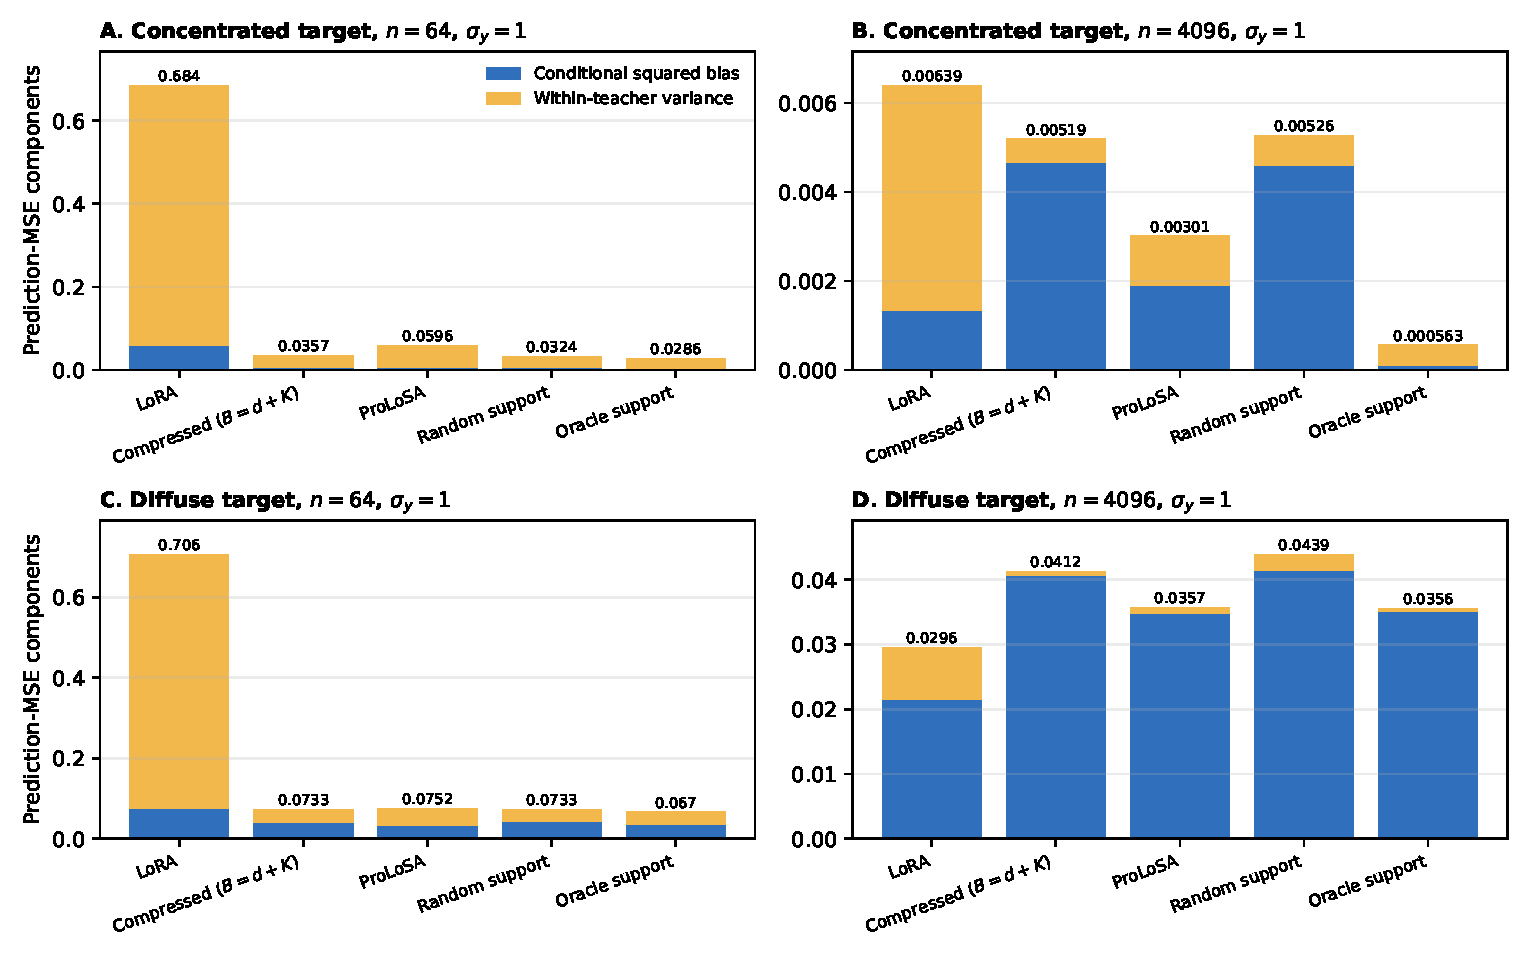
\includegraphics[width=0.9\textwidth]{transformer_biasvar.pdf}
    \caption{
    \textbf{Transformer teacher--student: function-space bias--variance
    decomposition} (Eq.~\eqref{eq:functional_bias_variance}, $\sigma_y=1$).
    Left column ($n=64$): variance dominates and compression removes it.
    Right column ($n=4096$): compressed parameterizations are pinned at their
    bias floors; sparse correction recovers a large fraction of the
    concentrated floor (top) but almost none of the diffuse floor (bottom),
    where even the oracle support fails, and the random-support hybrid does
    not improve on matched-budget compression.
    }
    \label{fig:transformer_biasvar}
\end{figure*}


\subsection{Testing the Downstream Predictions on Real Fine-Tuning}
\label{sec:real_model_validation}

The synthetic experiments establish the predicted mechanism under controlled assumptions.
We next examine three of its signatures in RoBERTa-large fine-tuning: the $1/n$ dependence of the compression advantage (E1), the bias--variance decomposition itself (E3), and the sparse recoverability of off-subspace residuals (E5).
Uni-LoRA and ProLoSA use matched compressed-parameter budgets, while rank-$4$ LoRA serves as the full-space baseline; all configurations follow Appendix Table~\ref{tab:glue_hyperparams}, and comparisons within each experiment share data subsets and evaluation sets.
Because Eq.~\eqref{eq:compressed_excess_risk} concerns predictive risk rather than raw parameter distance, E1 uses dev loss and E3 uses predictive probabilities as their primary observables.
For E5, we approximate the local curvature by the diagonal empirical Fisher,
$\hat H_{ii}=B^{-1}\sum_b(\partial\ell_b/\partial\theta_i)^2$, and weight residual coordinates after specifying the projection metric explicitly.

\begin{table*}[t]
\centering
\small
\caption{Real-model tests of the theoretical mechanism. E1 probes the sample-size signature in Eq.~\eqref{eq:risk_gap_n}; E3 decomposes predictive variability and a reference-based bias proxy; E5 diagnoses coordinate concentration related to the recoverability condition underlying Proposition~\ref{prop:matched_budget}.}
\label{tab:pred_overview}
\resizebox{\linewidth}{!}{%
\begin{tabular}{llll}
\toprule
Exp. & Theoretical target & Primary observable & Expected signature \\
\midrule
E1 & P1: sample-size scaling & $\Delta L_{\mathrm{dev}}(n)$ & positive $1/n$ component \\
E3 & bias--variance mechanism & $V_{\mathrm{stat}}$, $V_{\mathrm{opt}}$, $\mathrm{Bias}^2$ & compression lowers variance but raises bias \\
E5 & P4: sparse recoverability & Fisher-weighted residual capture & SNIP enrichment over random support \\
\bottomrule
\end{tabular}}
\end{table*}

\paragraph{E1: sample-size scaling (P1).}
We use fixed stratified subsets of fractions $p\in\{1\%,2\%,5\%,10\%,25\%,50\%,100\%\}$ on SST-2/QNLI and $p\in\{25\%,50\%,100\%\}$ on CoLA/MRPC. Each fraction uses subset seed 12345 for all methods and training seeds $s=0,\ldots,4$, with a fixed full-data update-step budget. For each run, dev loss is the minimum over its evaluation checkpoints, rather than a population-risk observation. We retain the dedicated-adapter-learning-rate LoRA reruns on SST-2/CoLA and the existing LoRA runs on QNLI/MRPC.
Define $\delta_s(p)=L_{L,s}(p)-L_{U,s}(p)$. We compute the mean and pointwise 95\% interval as
\begin{equation}
 \bar\delta(p)\ \pm\ t_{4,0.975}\,s_\delta(p)/\sqrt{5},
 \qquad s_\delta^2(p)=\tfrac14\sum_{s=0}^4(\delta_s(p)-\bar\delta(p))^2.
\end{equation}
The intervals in Table~\ref{tab:e1_paired_ci} use the paired differences themselves. They are conditional on the fixed subsets and dev set, reflect training randomness (including projection initialization), and are neither simultaneous intervals nor estimates of population sampling uncertainty.

We fit the same paired means to $a/n-b$ by unweighted least squares using actual subset sizes, both freely and with $a,b\geq0$ (Table~\ref{tab:e1_paired_fit}). All $5^5=3125$ ordered bootstrap resamples of complete seed trajectories give descriptive percentile intervals for both coefficients, retaining dependence across fractions. With only five trajectories, especially at a constraint boundary, these intervals are limited sensitivity estimates. Point residuals and bootstrap intervals for residual RMSE are retained in the reanalysis artifact.
SST-2's free fit has $\hat a=52.14$, $\hat b=-0.0171$, $R^2=0.485$, while CoLA's mean fit has $R^2=0.014$ on the same paired-mean scale. QNLI has $\hat a=-43.90$ with a bootstrap interval wholly below zero; imposing the theoretical signs gives $R^2=-0.363$. All four constrained point fits put $b$ at zero, so none yields a finite positive crossover. Negative slopes, structured residuals, and positive free intercepts indicate mismatch with the local asymptotic model under this protocol; an insufficient range of sample sizes alone does not explain them.

\begin{table*}[t]
\centering
\scriptsize
\setlength{\tabcolsep}{3pt}
\caption{\textbf{E1: sample-size scaling.} RoBERTa-large dev loss (mean$_{\pm\mathrm{std}}$ over 5 seeds). $\Delta=L_{\mathrm{dev}}^{\mathrm{LoRA}}-L_{\mathrm{dev}}^{\text{Uni-LoRA}}$; positive values favor compression.}
\label{tab:e1_crossover}
\begin{tabular}{lcccccccc}
\toprule
& \multicolumn{4}{c}{SST-2} & \multicolumn{4}{c}{QNLI} \\
\cmidrule(lr){2-5}\cmidrule(lr){6-9}
$p$ & LoRA & Uni-LoRA & ProLoSA & $\Delta(p)$ & LoRA & Uni-LoRA & ProLoSA & $\Delta(p)$ \\
\midrule
$1\%$   & $.445_{\pm.035}$ & $.378_{\pm.048}$ & $.382_{\pm.081}$ & $.067$  & $.710_{\pm.038}$ & $.750_{\pm.034}$ & $.765_{\pm.058}$ & $-.040$ \\
$2\%$   & $.361_{\pm.053}$ & $.263_{\pm.028}$ & $.314_{\pm.023}$ & $.098$  & $.559_{\pm.078}$ & $.482_{\pm.045}$ & $.564_{\pm.071}$ & $.078$ \\
$5\%$   & $.256_{\pm.054}$ & $.183_{\pm.030}$ & $.188_{\pm.011}$ & $.073$  & $.407_{\pm.059}$ & $.259_{\pm.022}$ & $.289_{\pm.031}$ & $.147$ \\
$10\%$  & $.178_{\pm.009}$ & $.156_{\pm.009}$ & $.155_{\pm.022}$ & $.023$  & $.250_{\pm.024}$ & $.225_{\pm.009}$ & $.212_{\pm.005}$ & $.025$ \\
$25\%$  & $.139_{\pm.011}$ & $.139_{\pm.010}$ & $.139_{\pm.010}$ & $-.000$ & $.192_{\pm.016}$ & $.179_{\pm.004}$ & $.179_{\pm.006}$ & $.013$ \\
$50\%$  & $.133_{\pm.006}$ & $.132_{\pm.005}$ & $.132_{\pm.006}$ & $.002$  & $.168_{\pm.005}$ & $.158_{\pm.002}$ & $.158_{\pm.002}$ & $.010$ \\
$100\%$ & $.127_{\pm.006}$ & $.125_{\pm.006}$ & $.127_{\pm.005}$ & $.002$  & $.160_{\pm.007}$ & $.148_{\pm.004}$ & $.148_{\pm.003}$ & $.012$ \\
\bottomrule
\end{tabular}
\end{table*}

\begin{table*}[t]
\centering\small
\caption{Paired E1 mean loss gaps and pointwise 95\% Student-$t$ intervals (five training seeds, four degrees of freedom). The training subset is fixed at each fraction; these intervals do not measure uncertainty over new training sets or new dev sets.}
\label{tab:e1_paired_ci}
\begin{tabular}{lrrrr}
\toprule
Task & Fraction & $n$ & Mean gap & 95\% interval \\
\midrule
SST-2 & 1\% & 673 & 0.0671 & [-0.0206, 0.1549] \\
SST-2 & 2\% & 1346 & 0.0975 & [0.0395, 0.1556] \\
SST-2 & 5\% & 3367 & 0.0735 & [-0.0177, 0.1647] \\
SST-2 & 10\% & 6734 & 0.0227 & [0.0077, 0.0377] \\
SST-2 & 25\% & 16837 & -0.0002 & [-0.0200, 0.0196] \\
SST-2 & 50\% & 33674 & 0.0018 & [-0.0106, 0.0143] \\
SST-2 & 100\% & 67349 & 0.0023 & [-0.0083, 0.0129] \\
QNLI & 1\% & 1047 & -0.0395 & [-0.0736, -0.0054] \\
QNLI & 2\% & 2094 & 0.0776 & [-0.0159, 0.1710] \\
QNLI & 5\% & 5237 & 0.1474 & [0.0548, 0.2400] \\
QNLI & 10\% & 10474 & 0.0250 & [-0.0006, 0.0507] \\
QNLI & 25\% & 26185 & 0.0131 & [-0.0074, 0.0335] \\
QNLI & 50\% & 52371 & 0.0102 & [0.0053, 0.0151] \\
QNLI & 100\% & 104743 & 0.0125 & [0.0075, 0.0175] \\
CoLA & 25\% & 2137 & 0.0362 & [-0.0794, 0.1517] \\
CoLA & 50\% & 4275 & 0.0669 & [-0.0158, 0.1497] \\
CoLA & 100\% & 8551 & 0.0224 & [-0.0083, 0.0531] \\
MRPC & 25\% & 917 & -0.0003 & [-0.1204, 0.1197] \\
MRPC & 50\% & 1834 & 0.0009 & [-0.0208, 0.0226] \\
MRPC & 100\% & 3668 & 0.0156 & [0.0008, 0.0303] \\
\bottomrule
\end{tabular}
\end{table*}

\begin{table*}[t]
\centering\scriptsize
\caption{Unweighted fits of paired mean gaps to $a/n-b$. Brackets are descriptive 95\% percentile intervals from all $5^5=3125$ resamples of complete seed trajectories. Constrained fits impose $a,b\geq0$; boundary intervals such as $[0,0]$ are a consequence of the constraint and the five observed seeds.}
\label{tab:e1_paired_fit}
\begin{tabular}{llrrrr}
\toprule
Task & Fit & $a$ [interval] & $b$ [interval] & RMSE & $R^2$ \\
\midrule
SST-2 & Free & 52.14 [11.02, 86.04] & -0.0171 [-0.0344, -0.0020] & 0.0270 & 0.485 \\
SST-2 & Constrained & 68.69 [36.95, 98.78] & 0.0000 [0.0000, 0.0000] & 0.0302 & 0.358 \\
QNLI & Free & -43.90 [-63.14, -29.14] & -0.0464 [-0.0618, -0.0356] & 0.0538 & 0.065 \\
QNLI & Constrained & 25.83 [0.00, 57.84] & 0.0000 [0.0000, 0.0000] & 0.0650 & -0.363 \\
CoLA & Free & 14.83 [-218.67, 278.07] & -0.0378 [-0.0910, 0.0229] & 0.0185 & 0.014 \\
CoLA & Constrained & 122.47 [0.00, 278.07] & 0.0000 [0.0000, 0.0229] & 0.0257 & -0.902 \\
MRPC & Free & -17.00 [-119.24, 85.23] & -0.0162 [-0.0564, 0.0240] & 0.0043 & 0.641 \\
MRPC & Constrained & 2.81 [0.00, 85.23] & 0.0000 [0.0000, 0.0278] & 0.0088 & -0.477 \\
\bottomrule
\end{tabular}
\end{table*}


\paragraph{E3: empirical bias--variance decomposition (mechanism).}
We use five independently drawn 80\% stratified subsets of the available training corpus (without replacement within a subset; subset seeds 101--105) and two training seeds (0, 1) per subset. The dev examples and their ordering remain fixed. Let $f_{bs}$ be the predictive-probability vector, $\bar f_b$ its seed mean, and $\bar f$ the grand mean. Write $\|u\|_N^2=N^{-1}\sum_{i,c}u_{ic}^2$ to average over examples and sum over classes. For $B=5,S=2$, the reported finite-replicate convention is
\begin{align}
 \widehat V_{\rm opt}&=\frac{1}{B(S-1)}\sum_{b,s}\|f_{bs}-\bar f_b\|_N^2,\\
 \widehat V_{\rm between}&=\frac{1}{B-1}\sum_b\|\bar f_b-\bar f\|_N^2,\qquad
 \widehat V_{\rm stat}=\max\{\widehat V_{\rm between}-\widehat V_{\rm opt}/S,0\}.
\end{align}
The subtraction removes within-subset variability leaking into the subset means under a nested replicate model. The same seed labels recur across subsets; a crossed data/seed sensitivity calculation, subtracting the estimated data--seed interaction divided by $S$ instead, gives signed data components $(0.00301,0.00057,0.00656)$ on CoLA and $(0.00890,0.00157,-0.00110)$ on MRPC (LoRA, Uni-LoRA, ProLoSA). The nested convention gives $-0.00115$ for MRPC ProLoSA before clipping; the displayed zero is not evidence that its statistical variance vanishes. Two seed levels make either variance-component estimate imprecise. Moreover, these are resampling diagnostics conditional on the observed corpus, not an independent-population estimate of the $1/n$ coefficient.
Within-subset variability includes initialization, minibatch order, optimization, and the projection seed, which defaults to the training seed. We retain the historical $V_{\rm opt}$ notation but label this full component as training-seed variance in the figure.

The reference $f^{\rm ref}$ averages eight full-data LoRA predictions per task: three rank-4 E4 runs and five retained rank-64 E3 reference runs. The original quality rule retains rank-64 references with dev score at least 85\% of the best reference score; it excludes five failed CoLA runs and no MRPC runs. This is dev-based reference selection. Squared bias is the plug-in proxy $\|\bar f-f^{\rm ref}\|_N^2$; finite-ensemble noise and dev selection remain, so its sum with corrected variance is not an unbiased risk estimate or an exact empirical decomposition.

On CoLA, $87.8\%$ of the LoRA-to-Uni-LoRA variance reduction is attributable to training seeds. On MRPC, ProLoSA lowers the bias proxy and total variance relative to Uni-LoRA; CoLA lacks this bias correction. Table~\ref{tab:e3_reference} replaces the reference by the rank-4-only and rank-64-only ensembles and all eight leave-one-reference-out ensembles. The complete bias ordering remains LoRA $<$ Uni-LoRA $<$ ProLoSA on CoLA and LoRA $<$ ProLoSA $<$ Uni-LoRA on MRPC in every case. This robustness concerns ordering, not identification of population bias.

\begin{table*}[t]
\centering
\small
\setlength{\tabcolsep}{5pt}
\caption{\textbf{E3: empirical bias--variance decomposition in predictive-probability space.} Values are per-example averages over five data resamples and two optimization seeds. $V_{\mathrm{stat}}$ is finite-replicate corrected, $V_{\mathrm{total}}=V_{\mathrm{opt}}+V_{\mathrm{stat}}$, and Total is the descriptive sum $\mathrm{Bias}^2+V_{\mathrm{total}}$. The zero data component for MRPC ProLoSA is clipped.}
\label{tab:e3_decomp}
\begin{tabular}{llccccc}
\toprule
Task & Method & $V_{\mathrm{opt}}$ & $V_{\mathrm{stat}}$ & $V_{\mathrm{total}}$ & $\mathrm{Bias}^2$ & Total \\
\midrule
CoLA & LoRA     & $.0593$ & $.0043$ & $.0636$ & $.0136$ & $.0772$ \\
     & Uni-LoRA & $.0326$ & $.0006$ & $.0332$ & $.0309$ & $\mathbf{.0641}$ \\
     & ProLoSA  & $.0306$ & $.0063$ & $.0369$ & $.0319$ & $.0688$ \\
\midrule
MRPC & LoRA     & $.0283$ & $.0091$ & $.0374$ & $.0124$ & $.0498$ \\
     & Uni-LoRA & $.0313$ & $.0013$ & $.0326$ & $.0219$ & $.0545$ \\
     & ProLoSA  & $.0303$ & $.0000$ & $.0303$ & $.0180$ & $\mathbf{.0483}$ \\
\bottomrule
\end{tabular}
\end{table*}

\begin{table*}[t]
\centering\small
\caption{Sensitivity of squared bias proxies to the full-data reference: mixed (3 rank-4 + 5 rank-64 runs), rank-4 only, rank-64 only, and the range over eight leave-one-reference-out ensembles. Ranges are sensitivity checks, not confidence intervals.}
\label{tab:e3_reference}
\begin{tabular}{llrrrr}
\toprule
Task & Method & Mixed & Rank 4 & Rank 64 & Leave-one-out range \\
\midrule
CoLA & LoRA & 0.01363 & 0.02275 & 0.01769 & [0.01328, 0.01523] \\
CoLA & Uni-LoRA & 0.03091 & 0.03195 & 0.03982 & [0.02972, 0.03503] \\
CoLA & ProLoSA & 0.03189 & 0.03440 & 0.03990 & [0.03081, 0.03594] \\
MRPC & LoRA & 0.01236 & 0.02146 & 0.01703 & [0.01184, 0.01426] \\
MRPC & Uni-LoRA & 0.02187 & 0.03247 & 0.02563 & [0.02103, 0.02418] \\
MRPC & ProLoSA & 0.01804 & 0.02927 & 0.02142 & [0.01762, 0.02003] \\
\bottomrule
\end{tabular}
\end{table*}


\paragraph{E5: residual geometry and coordinate-support reference (P4).}
We reanalyse the saved artifacts without retraining, explicitly averaging only full-data rank-4 LoRA targets: eight runs each on CoLA/MRPC and five each on QNLI/RTE/STS-B. Dedicated-learning-rate reruns replace superseded runs. We use the full-data seed-0 ProLoSA support in each task, chosen by this fixed provenance rule, rather than selecting the support with highest capture. All $D=1{,}769{,}472$ factor coordinates are candidate support positions; the stored offsets form a bijection to this ordering. CoLA/MRPC use $(d,K)=(14400,8640)$; the other tasks use $(22320,721)$ (the saved mask has 721 active entries although its nominal budget is 720). These are single-support diagnostics, not averages across support seeds or the MRPC configuration of E3. All reported energy fractions use this explicit full-data target/support selection.

Let $\bar\theta_L$ denote this mean factor-space target proxy. The original coordinate diagnostic forms the Euclidean residual
$q_E=(I-PP^\top)\bar\theta_L$ and then weights its coordinates by $\hat H_{ii}$.
The saved $\hat H$ averages squared minibatch-mean loss gradients over up to 200 training batches of size 16 (156 batches for RTE) at one full-data LoRA checkpoint per task. It is a diagonal sensitivity proxy, not an exact Hessian or the per-example Fisher. Factor coordinates and their cross-seed mean are gauge-dependent, which further limits identification with functional projection bias.
The metric projection instead gives
\begin{equation}
 q_H=\bar\theta_L-P(P^\top\hat H P)^\dagger P^\top\hat H\bar\theta_L.
\end{equation}
For one-hot sharing, $q_E$ subtracts the ordinary mean within each bucket, whereas $q_H$ subtracts its $\hat H$-weighted mean. Hence post-weighting an Euclidean residual does not compute an $H$-orthogonal residual.

For either fixed residual $q$, let $e_i=\hat H_{ii}q_i^2$ and $\rho_{I,H}^2=\sum_{i\in I}e_i/\sum_i e_i$. Uniform sampling of $K$ coordinates without replacement gives
\begin{equation}
 \mathbb E_I[\rho_{I,H}^2]
 =\frac{\sum_i\Pr(i\in I)e_i}{\sum_i e_i}=\frac KD.
\end{equation}
More generally, a candidate set $C$ gives $(K/|C|)\sum_{i\in C}e_i/\sum_i e_i$; residual-subspace dimension $D-d$ is not the number of original-coordinate candidates. Enrichment in Table~\ref{tab:e5_recoverability} therefore uses $K/D$. Table~\ref{tab:e5_random} directly checks this reference with 10,000 uniform supports per task. The sample means agree with $K/D$ within two Monte Carlo standard errors; the broad, asymmetric support distribution is reported separately from uncertainty in its mean.

Coordinate capture still differs from joint approximation-bias recovery, even on $q_H$. To measure the latter under the same diagonal proxy, we refit bucket means on the unselected coordinates and fit selected coordinates freely, computing
\begin{equation}
 \gamma_{I,H}=1-
 \frac{\min_{z,\alpha}\|\bar\theta_L-Pz-E_I\alpha\|_{\hat H}^2}
 {\|q_H\|_{\hat H}^2}.
\end{equation}
On MRPC, the $q_E$ coordinate fraction is $18.04\%$, the $q_H$ coordinate fraction is $2.67\%$, and $\gamma_{I,H}=5.68\%$ (Table~\ref{tab:e5_geometry}). The gap across these quantities is substantial. The latter holds $d$ fixed and is not the matched-budget benefit relative to a larger compressed space; it also omits training and support-selection noise. The observed coordinate enrichment supports a sensitivity diagnostic, not a direct verification of the population-energy condition in Proposition~\ref{prop:matched_budget}. Unweighted coordinate enrichment remains below one on all five tasks.

\begin{table*}[t]
\centering\small
\caption{E5 coordinate-energy diagnostics on an explicitly full-data LoRA target proxy. $q_E=(I-PP^\top)\Delta\theta$; oracle and SNIP capture fractions of $\sum_i\hat H_{ii}q_{E,i}^2$. The uniform-coordinate reference is $K/D$, $D=1{,}769{,}472$.}
\label{tab:e5_recoverability}
\begin{tabular}{lrrrrr}
\toprule
Task & $K$ & Oracle & SNIP & $K/D$ & Enrichment \\
\midrule
CoLA & 8640 & 0.4987 & 0.0791 & 0.004883 & $16.21\times$ \\
MRPC & 8640 & 0.6945 & 0.1804 & 0.004883 & $36.94\times$ \\
QNLI & 721 & 0.1446 & 0.0312 & 0.000407 & $76.52\times$ \\
RTE & 721 & 0.3374 & 0.0114 & 0.000407 & $27.98\times$ \\
STS-B & 721 & 0.5191 & 0.0791 & 0.000407 & $194.13\times$ \\
\bottomrule
\end{tabular}
\end{table*}

\begin{table*}[t]
\centering\scriptsize
\caption{Effect of projection geometry with the same target, Fisher diagonal, and saved SNIP support. Coordinate capture on $q_E$ and $q_H$ uses each residual's own total weighted energy. Joint recovery refits the compressed and sparse coefficients under the diagonal metric and is normalized by $\|q_H\|_{\hat H}^2$.}
\label{tab:e5_geometry}
\begin{tabular}{lrrrr}
\toprule
Task & Capture on $q_E$ & Capture on $q_H$ & Joint recovery & $\|q_H\|_{\hat H}^2/\|q_E\|_{\hat H}^2$ \\
\midrule
CoLA & 7.915\% & 1.188\% & 2.347\% & 0.767 \\
MRPC & 18.037\% & 2.667\% & 5.683\% & 0.567 \\
QNLI & 3.118\% & 0.138\% & 0.384\% & 0.836 \\
RTE & 1.140\% & 0.078\% & 0.239\% & 0.590 \\
STS-B & 7.910\% & 0.198\% & 0.874\% & 0.471 \\
\bottomrule
\end{tabular}
\end{table*}

\begin{table*}[t]
\centering\small
\caption{Uniform random-support check: 10,000 independent size-$K$ subsets drawn without replacement from all $D$ original coordinates (values in percent). The central 95\% range describes random-support variation; it is not an interval for the mean. The last column counts draws reaching the observed SNIP capture on $q_E$.}
\label{tab:e5_random}
\begin{tabular}{lrrrr}
\toprule
Task & Exact mean & Sample mean & Central 95\% range & Exceedances \\
\midrule
CoLA & 0.4883 & 0.4875 & [0.3639, 0.8057] & 0 \\
MRPC & 0.4883 & 0.4889 & [0.2586, 1.3675] & 0 \\
QNLI & 0.0407 & 0.0407 & [0.0259, 0.0838] & 0 \\
RTE & 0.0407 & 0.0402 & [0.0150, 0.1289] & 8 \\
STS-B & 0.0407 & 0.0420 & [0.0102, 0.1840] & 0 \\
\bottomrule
\end{tabular}
\end{table*}



\subsection{Synthetic Experiment Configuration}

Table~\ref{tab:synthetic_hyperparams} summarizes the configuration used for the projection-blind synthetic validation experiment in Appendix~\ref{sec:synthetic} and the bias-dominated failure experiment in Appendix~\ref{sec:synthetic_failure}.
The matched-budget comparison of Figure~\ref{fig:synthetic_matched_budget} reuses the identical target, projection, and per-trial noise realizations (same master seed), and adds a compressed-only estimator with a $B=48$-dimensional projection of the same construction, a hybrid with a uniformly random size-$32$ support redrawn per trial, and a hybrid with the oracle support given by the top-$32$ coordinates of the true off-subspace residual $(I-PP^\top)\theta^\star$.

\begin{table}[htbp]
\centering
\small
\begin{tabular}{lc}
\toprule
Hyperparameter & Value \\
\midrule
Full dimension \(D\) & 4096 \\
Compressed dimension \(d\) & 16 \\
Sparse budget \(K\) & 32 \\
Ground-truth prior (main) & sparse heavy-tailed mixture, Eq.~\eqref{eq:synthetic_gt} \\
Mixture sparsity \(\pi\) & 0.01 \\
Gaussian std.\ \(\tau_0\) & 0.005 \\
Student-\(t\) d.o.f.\ \(\nu\) / std.\ \(\tau_1\) & 3 / 0.5 \\
Ground-truth prior (failure regime) & dense Gaussian \(\mathcal{N}(0,\tau^2)\), \(\tau=0.125\) (Sec.~\ref{sec:synthetic_failure}) \\
Effective sample size \(n_{\mathrm{eff}}\) & 512 \\
Noise std.\ \(\sigma_y\) & grid over \([0.1, 2.0]\) \\
Number of trials \(M\) & 200 \\
Projection type & random orthonormal (QR of a Gaussian matrix) \\
Sparse support & top-\(K\) of post-warmup residual \(|y-PP^\top y|\) \\
Evaluation metric & population excess risk \\
Random seed & 13 \\
\bottomrule
\end{tabular}
\caption{Configuration of the projection-blind synthetic bias--variance validation and failure-regime experiments. For each regime, the target and column-orthonormal projection are drawn independently once and then fixed across all noise trials. Under the isotropic analysis of Appendix~\ref{app:energy_noise_condition}, the random orthonormal projection is exchangeable in expectation with the normalized one-hot construction used in the real-model experiments.}
\label{tab:synthetic_hyperparams}
\end{table}

\subsection{Transformer Teacher--Student Configuration}
\label{app:transformer_details}

Table~\ref{tab:transformer_hyperparams} lists the full configuration of the
Transformer teacher--student experiment of Appendix~\ref{sec:transformer_synthetic}.
The base parameters $W_0$ are pretrained once on a generic synthetic
sequence-regression task and shared by all methods, target profiles, and grid
cells; the teacher, planted update, projection, and training seeds are
controlled by separate deterministic seeds.
The concentrated and diffuse targets are planted directly in the vectorized
weight-update space $\operatorname{vec}(\Delta W_q,\Delta W_v)$ and rescaled
to the functional displacements in the table; the realized off-subspace
fractions are $0.991$ (concentrated) and $0.994$ (diffuse), with top-$K$
residual energy fractions of $0.988$ and $0.068$, respectively.

\begin{table}[htbp]
\centering
\small
\begin{tabular}{@{}p{0.35\linewidth}p{0.60\linewidth}@{}}
\toprule
Hyperparameter & Value \\
\midrule
Block & $d_{\mathrm{model}}=64$, $T=32$, $d_{\mathrm{ff}}=256$ \\
Adapted modules & $W_q$, $W_v$ \\
Update-space dimension $D$ & 8192 \\
LoRA rank & 4 (1024 trainable parameters) \\
Compressed budget $B=d+K$ & $128$ ($d=64$, $K=64$) \\
Target profiles & spike--slab ($\pi=0.01$, $\tau_0=0.005$, $t_3$ slab, std $0.5$); dense Gaussian \\
Functional displacement $\delta_{\mathrm{func}}$ & $10\%$ (concentrated) / $100\%$ (diffuse) \\
Optimizer & AdamW, lr $5\times10^{-3}$, $1000$ steps, batch size $128$, grad.\ clip $1.0$ \\
ProLoSA warmup / SNIP window & $10\%$ / $128$ steps \\
Grid & $n\in\{64,128,256,512,1024,4096\}$, $\sigma_y\in\{0.1,0.25,0.5,1,1.5,2\}$ \\
Seeds per cell & 20 (independent training sets and optimization seeds) \\
Evaluation & prediction MSE on $1024$ fixed noiseless teacher samples \\
Oracle support & top-$K$ of $\widehat H_{ii}(\theta_i^\star)^2$, diagonal empirical Gauss--Newton proxy \\
\bottomrule
\end{tabular}
\caption{Configuration of the Transformer teacher--student experiment.}
\label{tab:transformer_hyperparams}
\end{table}

Table~\ref{tab:transformer_floors} reports the functional approximation
floors obtained from noiseless large-sample fits ($n=8192$, $\sigma_y=0$),
which verify that the two profiles instantiate the recoverable and diffuse
regimes before the finite-sample grid is run.
Note that rank-$4$ LoRA also has a nonzero floor ($0.0011$ and $0.0235$):
the rank constraint is itself a form of compression, and the framework
applies to it in the same way (cf.\ Section~\ref{sec:conclusion}).

\begin{table}[htbp]
\centering
\small
\begin{tabular}{lcc}
\toprule
Parameterization & Concentrated target & Diffuse target \\
\midrule
Full fine-tuning & $2\times10^{-6}$ & $6\times10^{-6}$ \\
LoRA ($r=4$) & $0.0011$ & $0.0235$ \\
Compressed ($d=64$) & $0.0050$ & $0.0458$ \\
Compressed ($B=d+K=128$) & $0.0047$ & $0.0407$ \\
ProLoSA ($d=64$, $K=64$) & $0.0012$ & $0.0350$ \\
Random-support hybrid & $0.0041$ & $0.0431$ \\
Oracle-support hybrid & $6\times10^{-5}$ & $0.0353$ \\
\bottomrule
\end{tabular}
\caption{Functional approximation floors (noiseless, large-sample fits). The oracle hybrid removes $99\%$ of the compressed floor under the concentrated target but only $13\%$ under the diffuse target.}
\label{tab:transformer_floors}
\end{table}


\clearpage
\section{Downstream Benchmarks and Settings}
\label{app:downstream}
\label{app:exp_details}

This appendix provides implementation details omitted from the main text for reproducibility.
Unless otherwise specified, the pretrained backbone is frozen and only PEFT parameters are updated.
For each benchmark, all compared methods use the same data split, target modules, optimizer, batch size, number of epochs, learning-rate schedule, and random seeds whenever applicable.
For \textbf{ProLoSA}, the sparse support is selected after compressed warmup using the accumulated sensitivity score defined in Appendix~\ref{sec:routed_sparse_adapter}.
Unless a benchmark specifies otherwise (Llama-3.1 and ViT below), the reported warmup ratio $\rho_{\mathrm{w}}$ refers to the score-free compressed-only phase $T_{\mathrm{pre}}=\lfloor\rho_{\mathrm{w}}T\rfloor$; the sparse branch is activated only after the additional fixed $T_{\mathrm{s}}=128$-step scoring window, i.e., at step $\lfloor\rho_{\mathrm{w}}T\rfloor+128$.
The selected support is fixed during the remaining training stage, and the sparse coefficients are initialized to zero.
All reported training time and memory statistics include method-specific stages, including the warmup stage of \textbf{ProLoSA}.


\subsection{Main Results}

\paragraph{Results on GLUE.}
Table~\ref{tab:glue} reports the results on GLUE \citep{wang2018glue}. 
ProLoSA improves the average score of Uni-LoRA \citep{li2025unilora} from 85.3 to 85.5 on RoBERTa-base and from 88.3 to 88.7 on RoBERTa-large with the same trainable budget, achieving the best average among compressed baselines.
The stronger relative performance of compressed methods on RoBERTa-large than on RoBERTa-base (where full LoRA retains an edge) is qualitatively compatible with the variance-reduction interpretation; however, changing the backbone alters not only the full-space dimension $D$ but also the representation quality, curvature, gradient noise, and target update simultaneously, so we do not treat this comparison as a controlled test of Eq.~\eqref{eq:energy_noise_risks}---the controlled mechanism checks are reported in Appendix~\ref{sec:real_model_validation}.

\begin{table*}[t]
\centering
\caption{Results with RoBERTa$_{\text{base}}$ and RoBERTa$_{\text{large}}$ on GLUE \citep{wang2018glue}: Matthews correlation (CoLA), Pearson correlation (STS-B), and accuracy (others); mean$_{\pm\mathrm{std}}$ over 5 seeds. Baseline results are from Uni-LoRA \citep{li2025unilora}. $^\dagger$For VB-LoRA we quote the trainable-parameter count reported by the original paper, whose counting convention (stored vs.\ trained parameters) differs from the other rows.}
\label{tab:glue}
\resizebox{0.9\linewidth}{!}{%
\begin{tabular}{clcccccccc}
\toprule
Backbone & Method & Trainable Params & SST-2 & MRPC & CoLA & QNLI & RTE & STS-B & Avg. \\
\midrule
\multirow{8}{*}{\rotatebox[origin=c]{90}{BASE}} 
& FT & 125M & 94.8 & 90.2 & 63.6 & 92.8 & 78.7 & 91.2 & 85.2 \\
& LoRA & 0.295M & $\textbf{95.1}_{\pm 0.2}$ & $89.7_{\pm 0.7}$ & $63.4_{\pm 1.2}$ & $\textbf{93.3}_{\pm 0.3}$ & $\textbf{86.6}_{\pm 0.7}$ & $\textbf{91.5}_{\pm 0.2}$ & \textbf{86.6} \\
\cmidrule{2-10}
& VeRA & 0.043M & $94.6_{\pm 0.1}$ & $89.5_{\pm 0.5}$ & $\textbf{65.6}_{\pm 0.8}$ & $91.8_{\pm 0.2}$ & $78.7_{\pm 0.7}$ & $90.7_{\pm 0.2}$ & 85.2 \\
& Tied-LoRA & 0.043M & $94.4_{\pm 0.5}$ & $88.5_{\pm 1.0}$ & $61.9_{\pm 1.6}$ & $92.0_{\pm 0.4}$ & $76.2_{\pm 1.3}$ & $89.8_{\pm 0.3}$ & 83.8 \\
& VB-LoRA & 0.075M$^\dagger$ & $94.4_{\pm 0.2}$ & $89.5_{\pm 0.5}$ & $63.3_{\pm 0.7}$ & $92.2_{\pm 0.2}$ & $82.3_{\pm 1.3}$ & $90.8_{\pm 0.1}$ & 85.4 \\
& FourierFT & 0.024M & $94.2_{\pm 0.3}$ & $\textbf{90.0}_{\pm 0.8}$ & $63.8_{\pm 1.6}$ & $92.2_{\pm 0.1}$ & $79.1_{\pm 0.5}$ & $90.8_{\pm 0.2}$ & 85.0 \\
& Uni-LoRA & 0.023M & $94.5_{\pm 0.2}$ & $89.7_{\pm 0.4}$ & $64.6_{\pm 1.0}$ & $92.3_{\pm 0.4}$ & $79.8_{\pm 1.1}$ & $90.9_{\pm 0.2}$ & 85.3 \\
& ProLoSA & 0.023M & $94.9_{\pm 0.3}$ & $89.5_{\pm 0.6}$ & $63.5_{\pm 0.2}$ & $92.5_{\pm 0.2}$ & $81.7_{\pm 0.6}$ & $90.8_{\pm 0.2}$ & 85.5 \\
\midrule
\multirow{8}{*}{\rotatebox[origin=c]{90}{LARGE}} 
& LoRA & 0.786M & $96.2_{\pm 0.5}$ & $90.2_{\pm 1.0}$ & $68.2_{\pm 1.9}$ & $\textbf{94.8}_{\pm 0.3}$ & $85.2_{\pm 1.1}$ & $\textbf{92.3}_{\pm 0.5}$ & 87.8 \\
\cmidrule{2-10}
& VeRA & 0.061M & $96.1_{\pm 0.1}$ & $90.9_{\pm 0.7}$ & $68.0_{\pm 0.8}$ & $94.4_{\pm 0.2}$ & $85.9_{\pm 0.7}$ & $91.7_{\pm 0.8}$ & 87.8 \\
& Tied-LoRA & 0.066M & $94.8_{\pm 0.6}$ & $89.7_{\pm 1.0}$ & $64.7_{\pm 1.2}$ & $94.1_{\pm 0.1}$ & $81.2_{\pm 0.1}$ & $90.8_{\pm 0.3}$ & 85.9 \\
& VB-LoRA & 0.162M$^\dagger$ & $96.1_{\pm 0.2}$ & $91.4_{\pm 0.6}$ & $68.3_{\pm 0.7}$ & $94.7_{\pm 0.5}$ & $86.6_{\pm 1.3}$ & $91.8_{\pm 0.1}$ & 88.2 \\
& LoRA-XS & 0.025M & $95.9_{\pm 0.3}$ & $90.7_{\pm 0.4}$ & $67.0_{\pm 1.2}$ & $93.9_{\pm 0.1}$ & $\textbf{88.1}_{\pm 0.3}$ & $92.0_{\pm 0.1}$ & 87.9 \\
& FourierFT & 0.048M & $96.0_{\pm 0.2}$ & $90.9_{\pm 0.3}$ & $67.1_{\pm 1.4}$ & $94.4_{\pm 0.4}$ & $87.4_{\pm 1.6}$ & $92.0_{\pm 0.4}$ & 88.0 \\
& Uni-LoRA & 0.023M & $96.3_{\pm 0.2}$ & $91.3_{\pm 0.6}$ & $68.5_{\pm 1.1}$ & $94.6_{\pm 0.4}$ & $86.6_{\pm 1.6}$ & $92.1_{\pm 0.1}$ & $88.3$ \\
& ProLoSA & 0.023M & $\textbf{96.5}_{\pm 0.2}$ & $\textbf{91.7}_{\pm 0.6}$ & $\textbf{70.3}_{\pm 0.6}$ & $94.6_{\pm 0.1}$ & $87.4_{\pm 0.6}$ & $91.9_{\pm 0.2}$ & \textbf{88.7} \\
\bottomrule
\end{tabular}%
}
\end{table*}


\paragraph{Results on mathematical reasoning.}
Table~\ref{tab:math} reports results for Gemma-7B \citep{team2024gemma} on GSM8K \citep{cobbe2021training} and MATH \citep{hendrycks2021measuring}, and for Llama-3.1-8B on GSM8K and MATH500. On Gemma-7B, ProLoSA shows its main advantage on the harder MATH benchmark, improving over Uni-LoRA from 28.94 to 29.90 under the same 0.52M budget, while remaining competitive on GSM8K, where Uni-LoRA is strongest among all methods (75.59) and ProLoSA's sparse branch does not pay off (74.69).
On Llama-3.1-8B, LoRA ($r=64$, 167.77M parameters) achieves 79.61/33.20 on GSM8K/MATH500. At a shared 1.05M budget, Uni-LoRA achieves 75.44/26.20 and ProLoSA achieves 75.06/26.60: ProLoSA scores 0.40 points higher on MATH500 and 0.38 points lower on GSM8K. These single-seed results show a tradeoff rather than a consistent improvement; both compressed methods remain below rank-64 LoRA. The displayed compressed configurations maximize the two-benchmark mean within each method at this budget among the available runs; this is a post-hoc test-set summary, with the full sweep reported in Appendix~\ref{app:llama31_math_sweep}.
We treat these results purely as a practical benchmark: because the model is fine-tuned once on MetaMathQA and then evaluated on both benchmarks (Appendix~\ref{app:exp_details}), the two evaluations share a single training update, so per-benchmark differences cannot be attributed to differences in task-specific update energy; a theoretical attribution would require training separately on each task's data and measuring the corresponding curvature-weighted off-subspace energies, which we leave to the controlled experiments of Appendix~\ref{sec:real_model_validation}.
\begin{table}[t]
\centering
\small
\begin{tabular}{lccc}
\toprule
\multicolumn{4}{c}{\textit{Gemma-7B}} \\
\midrule
Method & Trainable Params & GSM8K & MATH \\
\midrule
LoRA        & 200M    & {74.90} & \textbf{31.28} \\
VeRA        & 1.90M   & 74.98 & 28.84 \\
FourierFT   & 0.59M   & 72.97 & 25.14 \\
Uni-LoRA    & 0.52M   & \textbf{75.59} & 28.94 \\
{ProLoSA}   & 0.52M   & 74.69 & 29.90    \\
\midrule
\multicolumn{4}{c}{\textit{Llama-3.1-8B}} \\
\midrule
Method & Trainable Params & GSM8K & MATH500 \\
\midrule
LoRA ($r=64$) & 167.77M & \textbf{79.61} & \textbf{33.20} \\
Uni-LoRA & 1.05M & 75.44 & 26.20 \\
ProLoSA ($d:K=12:1$) & 1.05M & 75.06 & 26.60 \\
\bottomrule
\end{tabular}
\caption{Mathematical reasoning exact-match accuracy (\%). Gemma-7B uses full MATH; Llama-3.1-8B uses MATH500. Llama results use seed 42, with compressed configurations selected as described in the text; 1.05M denotes exactly 1,048,576 trainable parameters.}
\label{tab:math}
\end{table}




\paragraph{Results on instruction tuning.}
Table~\ref{tab:instruction} in Appendix~\ref{app:exp_details} summarizes instruction tuning under the QLoRA recipe \citep{dettmers2023qlora}. On multi-turn MT-Bench \citep{zheng2023judging}, ProLoSA outperforms both Uni-LoRA and standard LoRA \citep{hu2022lora} while using orders of magnitude fewer trainable parameters than the latter ($4.25$ vs.\ $3.23$ on LLaMA2-7B and $4.72$ vs.\ $4.13$ on LLaMA2-13B with $0.3\%$ of the LoRA budget); on single-turn scores it is competitive with Uni-LoRA but remains below LoRA on the 7B model ($5.36$ vs.\ $5.62$).


\subsection{Ablation Study}
\label{sec:ablation}

We ablate three design choices on CoLA and MRPC under matched trainable-parameter budgets: budget allocation between the two branches, sparse support selection, and warmup ratio; full results are reported in Appendix~\ref{app:ablation} (Table~\ref{tab:ablation_budget_full}).
Neither pure compression nor pure sparsity is optimal: hybrid allocations outperform the sparse-only variant by a large margin (e.g., $69.62$ vs.\ $59.99$ CoLA Matthews correlation at $d{+}K=23040$) and improve over compressed-only on at least one task.
Under the same $d=22320$ and $K=720$, warmup SNIP support selection outperforms both random and accumulated-gradient supports ($69.62$ vs.\ $66.58$ and $67.95$ on CoLA), where the accumulated-gradient variant scores coordinates by $\sum_t|g_i^{(t)}|$ without the $\theta$-weighting of Eq.~\eqref{eq:warmup_snip_score}.
Under the idealized isotropic matched-budget model, a random support is expected to provide no systematic gain over pure compression (Corollary~\ref{cor:random_support}); in the real network it performs slightly worse than compressed-only ($66.58$ vs.\ $68.99$), which may reflect anisotropic curvature, optimization and conditioning effects of the augmented parameterization, or finite-sample variability.
The consistent ordering SNIP $>$ random supports the central prediction that the gain comes from \emph{informed residual allocation} rather than from sparsity itself.
Finally, varying the score-free warmup phase $T_{\mathrm{pre}}=\lfloor\rho_{\mathrm{w}}T\rfloor$ that precedes the fixed $128$-step scoring window, a ratio of $10\%$ performs best, whereas $20\%$ degrades both tasks, likely because the sparse branch is activated too late and the joint-optimization phase becomes too short.


\subsection{GLUE Hyperparameters}

Table~\ref{tab:glue_hyperparams} reports the main hyperparameters for GLUE.
We use the same settings for all compared PEFT methods under the corresponding backbone unless otherwise stated.
For CoLA, STS-B, and the remaining tasks, we report Matthews correlation, Pearson correlation, and accuracy, respectively.
The median performance over five random seeds is reported.

\begin{table}[htbp]
\centering
\footnotesize
\setlength{\tabcolsep}{2pt}
\begin{tabular}{llcccccc}
\toprule
Backbone & Task & $d$ & $K$ & Epochs & BS & LR \\
\midrule
RoBERTa-base  & SST-2 & 22320 & 720 & 60  & 32 & 5e-4 \\
RoBERTa-base  & MRPC  & 22320 & 720 & 30  & 32 & 1e-3 \\
RoBERTa-base  & CoLA  & 14400 & 8640 & 80  & 32 & 2e-2 \\
RoBERTa-base  & QNLI  & 22320 & 720 & 25  & 32 & 1e-3 \\
RoBERTa-base  & RTE   & 22320 & 720 & 160 & 32 & 1e-2 \\
RoBERTa-base  & STS-B & 22320 & 720 & 80  & 32 & 2e-4 \\
RoBERTa-large & SST-2 & 22320 & 720 & 20  & 32 & 1e-3 \\
RoBERTa-large & MRPC  & 22320 & 720 & 40  & 32 & 2e-4 \\
RoBERTa-large & CoLA  & 14400 & 8640 & 40  & 32 & 5e-3 \\
RoBERTa-large & QNLI  & 22320 & 720 & 20  & 32 & 5e-4 \\
RoBERTa-large & RTE   & 22320 & 720 & 40  & 32 & 5e-3 \\
RoBERTa-large & STS-B & 22320 & 720 & 40  & 32 & 2e-4 \\
\midrule
Optimizer & \multicolumn{6}{c}{AdamW} \\
Scheduler & \multicolumn{6}{c}{Linear} \\
Seeds & \multicolumn{6}{c}{5} \\
ProLoSA warmup ratio & \multicolumn{6}{c}{10\%} \\
SNIP score-collection window & \multicolumn{6}{c}{128 steps}\\
\bottomrule
\end{tabular}
\caption{Core hyperparameter settings for GLUE experiments. BS denotes batch size. The $d$ and $K$ columns denote the compressed latent dimension and sparse residual budget used by ProLoSA.}
\label{tab:glue_hyperparams}
\end{table}

\subsection{Mathematical Reasoning Hyperparameters}

Table~\ref{tab:math_hyperparams} reports the Gemma-7B configuration for GSM8K and MATH.
Within each backbone, all methods use the same target modules, numerical precision, and decoding protocol; the Llama-3.1-8B settings and sweep are reported below.
Exact-match scores are computed with the same answer extraction rule for all methods.

\begin{table}[htbp]
\centering
\small
\setlength{\tabcolsep}{6pt}
\begin{tabular}{lcc}
\toprule
\textbf{Hyperparameter} & \textbf{GSM8K} & \textbf{MATH} \\
\midrule
\multicolumn{3}{c}{\textit{Shared Training Configuration}} \\
\midrule
Backbone & \multicolumn{2}{c}{Gemma-7B} \\
Train data & \multicolumn{2}{c}{MetaMathQA train} \\
Epochs & \multicolumn{2}{c}{2} \\
Train batch size & \multicolumn{2}{c}{1} \\
Gradient accumulation & \multicolumn{2}{c}{64} \\
Learning rate & \multicolumn{2}{c}{$2\times10^{-4}$} \\
Scheduler & \multicolumn{2}{c}{Cosine} \\
Max sequence length & \multicolumn{2}{c}{512} \\
ProLoSA $d$ & \multicolumn{2}{c}{349525} \\
ProLoSA $K$ & \multicolumn{2}{c}{174763} \\
ProLoSA warmup ratio & \multicolumn{2}{c}{10\%} \\
SNIP score-collection window & \multicolumn{2}{c}{128 steps}\\
Seeds & \multicolumn{2}{c}{42} \\
\midrule
\multicolumn{3}{c}{\textit{Task-Specific Evaluation Configuration}} \\
\midrule
Metric & \multicolumn{2}{c}{Exact match} \\
Eval batch size & 32 & 32 \\
Max new tokens & 1024 & 2048 \\
\bottomrule
\end{tabular}
\caption{Core training and evaluation settings for mathematical reasoning experiments. The model is fine-tuned once on MetaMathQA and evaluated across both benchmarks.}
\label{tab:math_hyperparams}
\end{table}


\paragraph{Llama-3.1-8B configuration and sweep.}
\label{app:llama31_math_sweep}
We fine-tune the Llama-3.1-8B base model (NousResearch mirror) on the first 100,000 MetaMathQA training examples for two epochs, using BF16 without weight quantization, a maximum training length of 512, batch size 1, gradient accumulation 64, cosine learning-rate decay, a 2\% scheduler warmup, and zero weight decay. All methods target the attention and MLP linear projections. LoRA uses $r=64$, $\alpha=64$, and learning rate $2\times10^{-4}$; Uni-LoRA and ProLoSA use $r=4$. Evaluation uses greedy decoding (temperature 0, top-$p=1$), batch size 32, and at most 1,024/2,048 generated tokens for GSM8K/MATH500. Each evaluated configuration uses seed 42 and the same fine-tuned checkpoint across the two benchmarks (1,319 and 500 examples, respectively); full MATH results are unavailable for this backbone.

In Table~\ref{tab:math}, Uni-LoRA uses $d=1{,}048{,}576$ and learning rate $2\times10^{-3}$. ProLoSA uses $d=967{,}916$, $K=80{,}660$ (approximately $12:1$), and a projected-vector learning rate of $1.6\times10^{-3}$. Its base learning rate is $2\times10^{-4}$, with sparse learning-rate multiplier 0.2, sparse warmup 128 steps, a one-step SNIP mask-collection window, and optimizer reset on mask activation. Its trainable budget counts both $d$ and $K$, including the sparse parameters activated after warmup.

Table~\ref{tab:llama31_math_sweep} lists all completed Llama-3.1-8B configurations found in the local evaluation results. At the shared 1,048,576-parameter budget, we display in the main table the configuration with the largest arithmetic mean of GSM8K and MATH500 for each compressed method. This descriptive selection uses the reported test scores, not an independent validation set; it does not establish statistical significance or a multi-seed advantage. The larger-budget Uni-LoRA runs and alternative ProLoSA ratios are retained below so that budget and hyperparameter effects remain visible.

\begin{table}[p]
\centering
\small
\setlength{\tabcolsep}{5pt}
\begin{tabular}{lrrrrr}
\toprule
Method & Params & $d:K$ & Learning rate & GSM8K & MATH500 \\
\midrule
LoRA ($r=4$) & 10,485,760 & -- & $2\times10^{-4}$ & 75.59 & 26.80 \\
LoRA ($r=64$) & 167,772,160 & -- & $2\times10^{-4}$ & 79.61 & 33.20 \\
\midrule
Uni-LoRA & 262,144 & -- & $2\times10^{-3}$ & 70.28 & 23.40 \\
Uni-LoRA & 524,288 & -- & $5\times10^{-4}$ & 68.39 & 25.40 \\
Uni-LoRA & 524,288 & -- & $1\times10^{-3}$ & 72.33 & 23.00 \\
Uni-LoRA & 524,288 & -- & $2\times10^{-3}$ & 73.84 & 24.80 \\
Uni-LoRA & 524,288 & -- & $4\times10^{-3}$ & 74.15 & 26.60 \\
Uni-LoRA & 524,288 & -- & $8\times10^{-3}$ & 74.75 & 24.20 \\
Uni-LoRA & 524,288 & -- & $1\times10^{-2}$ & 72.40 & 21.00 \\
Uni-LoRA & 1,048,576 & -- & $5\times10^{-4}$ & 72.25 & 25.00 \\
Uni-LoRA & 1,048,576 & -- & $1\times10^{-3}$ & 74.22 & 26.20 \\
Uni-LoRA & 1,048,576 & -- & $2\times10^{-3}$ & 75.44 & 26.20 \\
Uni-LoRA & 1,048,576 & -- & $4\times10^{-3}$ & 74.07 & 25.60 \\
Uni-LoRA & 2,097,152 & -- & $5\times10^{-4}$ & 74.45 & 26.00 \\
Uni-LoRA & 2,097,152 & -- & $1\times10^{-3}$ & 75.97 & 25.60 \\
Uni-LoRA & 2,097,152 & -- & $2\times10^{-3}$ & 76.95 & 26.00 \\
Uni-LoRA & 2,097,152 & -- & $4\times10^{-3}$ & 74.30 & 25.80 \\
Uni-LoRA & 4,194,304 & -- & $2\times10^{-3}$ & 76.12 & 26.20 \\
\midrule
ProLoSA & 524,288 & 2:1 & $8\times10^{-4}$ & 69.75 & 24.80 \\
ProLoSA & 524,288 & 4:1 & $8\times10^{-4}$ & 69.07 & 21.40 \\
ProLoSA & 524,288 & 8:1 & $8\times10^{-4}$ & 69.83 & 21.00 \\
ProLoSA & 524,288 & 12:1 & $4\times10^{-4}$ & 68.23 & 21.00 \\
ProLoSA & 524,288 & 12:1 & $8\times10^{-4}$ & 71.27 & 21.00 \\
ProLoSA & 524,288 & 12:1 & $1.6\times10^{-3}$ & 73.31 & 20.60 \\
ProLoSA & 524,288 & 12:1 & $3.2\times10^{-3}$ & 73.92 & 23.80 \\
ProLoSA & 1,048,576 & 2:1 & $1.6\times10^{-3}$ & 73.77 & 24.80 \\
ProLoSA & 1,048,576 & 2:1 & $3.2\times10^{-3}$ & 74.98 & 24.60 \\
ProLoSA & 1,048,576 & 4:1 & $1.6\times10^{-3}$ & 75.66 & 24.80 \\
ProLoSA & 1,048,576 & 4:1 & $3.2\times10^{-3}$ & 74.60 & 25.00 \\
ProLoSA & 1,048,576 & 8:1 & $1.6\times10^{-3}$ & 74.07 & 26.20 \\
ProLoSA & 1,048,576 & 8:1 & $3.2\times10^{-3}$ & 74.37 & 25.60 \\
ProLoSA & 1,048,576 & 12:1 & $1.6\times10^{-3}$ & 75.06 & 26.60 \\
ProLoSA & 1,048,576 & 12:1 & $3.2\times10^{-3}$ & 74.53 & 21.60 \\
\bottomrule
\end{tabular}
\caption{Complete available Llama-3.1-8B sweep (exact-match accuracy in \%, seed 42). The learning-rate column gives the projected-vector rate for ProLoSA, whose base rate is fixed at $2\times10^{-4}$, and the optimizer rate for LoRA/Uni-LoRA. Ratios $d:K$ are approximate due to integer budgets. Rank-4 LoRA is included only as a supplementary reference; the main baseline uses rank 64. Each row reports both benchmarks from one configuration.}
\label{tab:llama31_math_sweep}
\end{table}

\subsection{Instruction-Tuning Hyperparameters}

Table~\ref{tab:instruction} reports the full instruction-tuning results referenced in the main text, and Table~\ref{tab:instruction_hyperparams} reports the core configuration.
All methods are trained on the same instruction data and evaluated with the same MT-Bench protocol.
For QLoRA-style experiments, the backbone is quantized and frozen, and only PEFT parameters are updated.

\begin{table}[htbp]
\centering
\small
\begin{tabular}{lccc}
\toprule
\textbf{Method} & \textbf{\# Params} & \textbf{Score$_1$} & \textbf{Score$_2$} \\
\midrule
w/o FT       & -       & 1.31 / 1.46 & 1.11 / 1.06 \\
LoRA$^{\#}$  & 159.9M / 250.3M & \textbf{5.62} / 6.20 & 3.23 / 4.13 \\
Uni-LoRA     & 0.52M / 1.0M    & 5.34 / 6.34 & 3.56 / 4.43 \\
ProLoSA      & 0.52M / 1.0M    & 5.36 / \textbf{6.57} & \textbf{4.25} / \textbf{4.72} \\
\bottomrule
\end{tabular}
\caption{
Instruction-tuning results under the QLoRA training recipe \citep{dettmers2023qlora}. 
Each entry reports LLaMA2-7B / LLaMA2-13B results. 
Score$_1$ and Score$_2$ denote MT-Bench single-turn and multi-turn scores, respectively.
}
\label{tab:instruction}
\end{table}

\begin{table}[t]
\centering
\small
\renewcommand{\arraystretch}{0.9} % 稍微压缩行距，节省纵向空间
\setlength{\tabcolsep}{4pt}
\begin{tabular}{lcc}
\toprule
Hyperparameter & Shared / LLaMA2-7B & LLaMA2-13B \\
\midrule
Training data & \multicolumn{2}{c}{Cleaned Alpaca} \\
Evaluation & \multicolumn{2}{c}{MT-Bench} \\
Quantization & \multicolumn{2}{c}{4-bit NF4 + double quantization} \\
Epochs & \multicolumn{2}{c}{1} \\
Effective batch size & \multicolumn{2}{c}{16} \\
Per-device batch size & 4 & 2 \\
Gradient accumulation & 4 & 8 \\
Scheduler & \multicolumn{2}{c}{Linear} \\
Max sequence length & \multicolumn{2}{c}{16 / 512} \\
Decoding strategy & \multicolumn{2}{c}{Category-specific sampling/greedy} \\
Temperature & \multicolumn{2}{c}{0.7 / 0.1 / 0 by category} \\
Max new tokens & \multicolumn{2}{c}{1024} \\
Evaluator / judge & \multicolumn{2}{c}{GPT-4 single} \\
LoRA params & 159.9M & 250.3M \\
Uni-LoRA params & 0.52M & 1.0M \\
ProLoSA params & 0.52M & 1.0M \\
ProLoSA $d$ & 507904 & 983040 \\
ProLoSA $K$ & 16384 & 65536 \\
ProLoSA warmup ratio & \multicolumn{2}{c}{10\%} \\
SNIP score-collection window & \multicolumn{2}{c}{128 steps}\\
Seeds & \multicolumn{2}{c}{0} \\
\bottomrule
\end{tabular}
\caption{Core training and evaluation settings for instruction-tuning experiments. Score$_1$ and Score$_2$ denote MT-Bench single-turn and multi-turn scores, respectively.}
\label{tab:instruction_hyperparams}
\end{table}

\subsection{Ablation Details}
\label{app:ablation}

Table~\ref{tab:ablation_budget_full} reports the full budget-allocation sweep between the projected branch and the sparse residual branch.
All variants use the same total trainable-parameter budget $B=d+K=23040$.
The compressed-only variant corresponds to $K=0$, the sparse-only variant corresponds to $d=0$, and intermediate configurations correspond to \textbf{ProLoSA} with both branches active.
Since $B$ is fixed, increasing the sparse budget $K$ necessarily reduces the compressed latent dimension $d$.

\begin{table}[t]
\centering
\small
\renewcommand{\arraystretch}{0.9} % 纵向稍微压缩行距，节省高度
\setlength{\tabcolsep}{2.5pt}     % 缩小列与列之间的空白间距，避免缩小字号
\begin{tabular}{@{}llcccc@{}}      % @{} 去除表格最左和最右的额外空白占位
\toprule
Study & Variant & $d$ & $K$ & CoLA & MRPC \\
\midrule
\multirow{9}{*}{Budget}
& Compressed-only & 23040 & 0     & $68.99_{\pm 0.58}$ & $90.93_{\pm 0.00}$ \\
& ProLoSA & 22680 & 360   & $68.29_{\pm 1.40}$ & $90.11_{\pm 0.50}$ \\
& ProLoSA & 22320 & 720   & $69.62_{\pm 1.84}$ & $\mathbf{91.69}_{\pm 0.40}$ \\
& ProLoSA & 21600 & 1440  & $67.21_{\pm 0.84}$ & $90.87_{\pm 0.46}$ \\
& ProLoSA & 20160 & 2880  & $68.72_{\pm 0.45}$ & $83.74_{\pm 9.65}$ \\
& ProLoSA & 18720 & 4320  & $67.51_{\pm 0.51}$ & $90.03_{\pm 0.42}$ \\
& ProLoSA & 14400 & 8640  & $\mathbf{70.27}_{\pm 0.60}$ & $90.77_{\pm 0.42}$ \\
& ProLoSA & 5760  & 17280 & $68.75_{\pm 1.27}$ & $89.71_{\pm 0.20}$ \\
& Sparse-only & 0 & 23040 & $59.99_{\pm 1.40}$ & $84.89_{\pm 0.83}$ \\
\midrule
\multirow{3}{*}{Support}
& Random & 22320 & 720 & $66.58_{\pm 0.63}$ & $90.28_{\pm 0.61}$ \\
& Accum. gradient & 22320 & 720 & $67.95_{\pm 0.59}$ & $90.03_{\pm 0.31}$ \\
& Warmup SNIP & 22320 & 720 & $\mathbf{69.62}_{\pm 1.84}$ & $\mathbf{91.69}_{\pm 0.40}$ \\
\midrule
\multirow{4}{*}{Warmup}
& $0\%$ & 22320 & 720 & $67.32_{\pm 0.47}$ & $90.36_{\pm 0.20}$ \\
& $5\%$ & 22320 & 720 & $69.05_{\pm 0.51}$ & $91.12_{\pm 0.70}$ \\
& $10\%$ & 22320 & 720 & $\mathbf{69.62}_{\pm 1.84}$ & $\mathbf{91.69}_{\pm 0.40}$ \\
& $20\%$ & 22320 & 720 & $67.49_{\pm 0.96}$ & $90.60_{\pm 0.81}$ \\
\bottomrule
\end{tabular}
\caption{
Ablation details on budget allocation, sparse support selection, and warmup length.
CoLA reports Matthews correlation and MRPC reports accuracy.
}
\label{tab:ablation_budget_full}
\end{table}

\clearpage
\subsection{Vision Transformer Experiments}
\label{app:vit}

\paragraph{Relation to the original vision experiments.}
Uni-LoRA \citep{li2025unilora} already evaluates ViT-Base and ViT-Large on eight image-classification datasets, with five runs per configuration (its Section~4.4 and Table~5). We extend this line of evaluation to ProLoSA using the completed ViT-B/16 runs. Our data subsets, optimization settings, and seed coverage differ from that study, so all LoRA and Uni-LoRA scores in Table~\ref{tab:vit} come from the same local experiment suite as ProLoSA. They are not copied from the original paper. No completed ProLoSA ViT-Large results are available in this suite.

\paragraph{Model and data.}
We use the ImageNet-21k-pretrained ViT-B/16 checkpoint (\path{google/vit-base-patch16-224-in21k}) and apply rank-4 adapters to query and value projections in all 12 Transformer blocks. All other backbone parameters are frozen, and a randomly initialized classification head is trained for every method. The three limited-data settings use 1,000 training images from CIFAR-100, Food-101, and DTD, respectively. Sampling is stratified by class with subset seed 42, giving 10 images per class for CIFAR-100 and approximately balanced allocations for Food-101 and DTD. CIFAR-100 additionally uses 5,000 images and the full 50,000-image training split. These are custom stratified subsets, not the standard VTAB-1k protocol. Evaluation uses the complete CIFAR-100 test split (10,000 images), Food-101 validation split (25,250), and DTD test split (1,880), respectively. Training applies random resized cropping to $224\times224$, horizontal flipping, and pretrained-model normalization; evaluation uses resizing, center cropping, and the same normalization.

\paragraph{Budgets and parameter accounting.}
The rank-4 LoRA factor space contains $D=12\times2\times(768\times4+4\times768)=147{,}456$ parameters. Uni-LoRA uses $d=24{,}600$, while ProLoSA divides the same budget into $d+K=24{,}600$ (Table~\ref{tab:vit_allocations}). The shared head adds $769C$ parameters for $C$ classes: 76,900 for CIFAR-100, 77,669 for Food-101, and 36,143 for DTD. Thus the total active parameter counts for either compressed method are 101,500, 102,269, and 60,743, respectively; LoRA totals are 224,356, 225,125, and 183,599. Adapter-only compression is approximately $6\times$; this factor does not apply to the totals including the head. ProLoSA counts the $K$ selected sparse coefficients even though they are frozen during warmup. The raw result files count parameters before activation and therefore contain only $d$ in their ProLoSA adapter field; we recover $d+K$ from the logged configuration and verify $K$ against the activation log. These counts describe active degrees of freedom, not allocated tensor storage or optimizer memory.

\begin{table}[t]
\centering\small
\begin{tabular}{lrr@{\qquad}lrr}
\toprule
\multicolumn{3}{c}{Main budget: $d+K=24{,}600$} & \multicolumn{3}{c}{Supplementary budget: $d+K=72{,}000$} \\
\cmidrule(lr){1-3}\cmidrule(lr){4-6}
Method & $d$ & $K$ & Method & $d$ & $K$ \\
\midrule
Uni-LoRA & 24,600 & 0 & Uni-LoRA & 72,000 & 0 \\
ProLoSA ($2:1$) & 16,400 & 8,200 & ProLoSA ($2:1$) & 48,000 & 24,000 \\
ProLoSA ($4:1$) & 19,680 & 4,920 & ProLoSA ($4:1$) & 57,600 & 14,400 \\
ProLoSA ($8:1$) & 21,867 & 2,733 & ProLoSA ($8:1$) & 64,000 & 8,000 \\
ProLoSA ($12:1$) & 22,708 & 1,892 & ProLoSA ($12:1$) & 66,462 & 5,538 \\
\bottomrule
\end{tabular}
\caption{Exact compressed-adapter budgets for ViT-B/16. Ratios are approximate when integer rounding is required. The task-specific classification head is additional and shared across methods.}
\label{tab:vit_allocations}
\end{table}

\paragraph{Optimization and support selection.}
All runs use AdamW with $(\beta_1,\beta_2)=(0.9,0.999)$, $\epsilon=10^{-8}$, zero weight decay, BF16, batch size 64, and no gradient accumulation. The 1,000-image settings train for 20 epochs (320 optimizer steps); CIFAR-100 with 5,000 and 50,000 images trains for 10 epochs (790 and 7,820 steps). LoRA uses $\alpha=r=4$ and adapter learning rate $10^{-3}$; Uni-LoRA and ProLoSA use a latent-vector learning rate of $4\times10^{-3}$. The head learning rate is $3\times10^{-3}$ for every method. Adapter dropout is zero. The latent/head learning rates follow linear decay with 10\% scheduler warmup. ProLoSA uses latent initialization bound 0.02, a score-free warmup of 32 steps for the 1,000-image settings or 128 steps otherwise, and a one-step SNIP scoring window. Its support is activated after step 33 or 129, respectively, with zero-initialized sparse coefficients and cleared optimizer state. The sparse learning rate is $0.2$ times the latent rate ($8\times10^{-4}$), with linear decay after activation. This support-selection schedule differs from the 128-step scoring window used in the earlier language experiments.

\paragraph{Reporting and limitations.}
We report \emph{final-model} top-1 accuracy, using the \texttt{final\_accuracy} field rather than \texttt{best\_accuracy}, which is the maximum over repeated evaluations on the same held-out split. The full method-by-setting comparison is available only for training seed 42, and Table~\ref{tab:vit} retains all four ProLoSA ratios. Only LoRA on CIFAR-100 with 1,000 images has additional completed seeds: its final accuracies for seeds 42/43/44 are 86.91/86.57/86.44. We therefore do not attach multi-seed error bars to the compressed-method comparison. No independent validation split was used to choose between the available budget/learning-rate recipes, so the highlighted recipe is an exploratory result. Full-data CIFAR-100 improves by 0.23 points over Uni-LoRA at $d:K=4:1$, but the four ProLoSA ratios lose 0.09--0.25 points at 1,000 images and 0.19--0.42 points at 5,000 images. The small Food-101 and DTD differences and the lack of repeated ProLoSA seeds preclude a consistent-advantage claim. The changing epoch count and number of updates across data sizes also prevent a controlled test of the sample-size law.

\paragraph{Supplementary 72,000-parameter recipe.}
Table~\ref{tab:vit_72k} retains the second complete single-seed sweep. It uses $d=72{,}000$ for Uni-LoRA and $d+K=72{,}000$ for ProLoSA, with latent learning rate $10^{-2}$, sparse learning rate $2\times10^{-3}$, and head learning rate $10^{-2}$ on CIFAR-100 or $5\times10^{-2}$ on Food-101 and DTD. LoRA's adapter learning rate remains $10^{-3}$; data, epochs, and support-selection timing are unchanged. Since the learning rates change together with the compressed budget (including the head rate for LoRA), differences from Table~\ref{tab:vit} do not isolate a budget effect. At this recipe, ProLoSA's $2:1$ allocation exceeds Uni-LoRA on the four limited-data settings but loses on full-data CIFAR-100; LoRA remains stronger than this allocation on Food-101, DTD, and the larger CIFAR-100 subsets. This recipe dependence reinforces the need for independent tuning and repeated seeds.

\begin{table}[t]
\centering\small
\setlength{\tabcolsep}{5pt}
% Generated from final_accuracy, seed 42; do not edit.
\begin{tabular}{lrrrrr}
\toprule
 & \multicolumn{3}{c}{1,000 training images} & \multicolumn{2}{c}{CIFAR-100} \\
\cmidrule(lr){2-4}\cmidrule(lr){5-6}
Method & CIFAR-100 & Food-101 & DTD & 5,000 & Full \\
\midrule
LoRA ($r=4$) & 85.22 & 73.52 & 68.83 & 89.32 & 91.78 \\
Uni-LoRA & 85.10 & 72.68 & 66.70 & 88.24 & 91.51 \\
ProLoSA ($2:1$) & 85.38 & 72.77 & 67.93 & 88.96 & 91.43 \\
ProLoSA ($4:1$) & 85.08 & 71.95 & 68.19 & 88.55 & 91.80 \\
ProLoSA ($8:1$) & 84.79 & 72.48 & 68.09 & 88.60 & 91.57 \\
ProLoSA ($12:1$) & 84.98 & 72.37 & 67.93 & 88.72 & 91.76 \\
\bottomrule
\end{tabular}

\caption{Supplementary ViT-B/16 recipe: final-model accuracy (\%, seed 42), with 72,000 active adapter parameters for both compressed methods and 147,456 for LoRA, plus the shared classification head. All available ProLoSA ratios are retained. Learning rates differ from the main vision table as specified in the text.}
\label{tab:vit_72k}
\end{table}


\end{document}
